\documentclass[fleqn, final]{../styles/unmphythesis}
\usepackage{../styles/qxd}
\renewcommand{\thechapter}{4}
%\newcommand{\thechapter}{1}

\makeindex
\begin{document}

%<*birefringenceprotocol>

\chapter{QND measurement and spin squeezing using the birefringence effect}\label{chap:birefringence}
\section{Introduction}

Strong coupling between atoms and photons is at the heart of many quantum information processing protocols including efficient generation of remote entanglement \cite{duan_long-distance_2001, julsgaard_experimental_2001}, quantum data storage and retrieval \cite{ eisaman_electromagnetically_2005}, and QND measurements \cite{eckert_quantum_2008}.  
From a general perspective, strong coupling arises when atoms radiate predominantly into the electromagnetic field mode that defines the quantum atom-light interface.  
For an individual atom, the strong coupling regime is attained via the Purcell effect, whereby the boundary conditions of nearby dielectrics and/or conductors enhance radiation into a desired mode relative to all other modes.  
This can be achieved with Fabry-Perot cavities (cavity QED) \cite{miller_trapped_2005} and/or via nanophotonic structures engineered such that the radiation is predominantly into a specified mode \cite{MangaRao2007Single, hakuta_manipulating_2012, hung_trapped_2013}.  The Purcell enhancement factors for emission into a guided or cavity mode scale respectively as  $ \Gamma_{\oneD}/\Gamma_{\vac} \sim \sigma_0/A$ and  $\Gamma_{\cav}/\Gamma_{\vac} \sim   Q \lambda^3/V \sim \mathcal{F}  \sigma_0/A$.  Here $\Gamma_{\vac}$ is the free space spontaneous emission rate, $\sigma_0 \propto \lambda^2$ is the resonant absorption cross section, $Q$, $V$, and $\mathcal{F}$,  are the cavity quality factor, volume, and finesse respectively, and $A$ is the effective area of the cavity or guided mode that couples to the atom.  The strongest coupling occurs on resonance, and thus much effort has been devoted to developing the largest possible $\Gamma_{\cav}$ and $\Gamma_{\oneD}$ through ultra-high-$Q$, small-volume resonators \cite{raimond_manipulating_2001, wallraff_strong_2004, miller_trapped_2005} and through nanophotonic plasmonic \cite{dzsotjan_quantum_2010, tame_quantum_2013}, metamaterial \cite{yao_ultrahigh_2009}, and dielectric \cite{hung_trapped_2013, goban_atomlight_2014} waveguides.   

In free space, where there is no Purcell enhancement, strong coupling can be achieved via the {\em cooperativity} of atomic ensembles.  
This is most naturally implemented in a dispersive regime, off resonance, where light elastically scattered from the ensemble constructively interferes to match the mode of an exciting paraxial probe \cite{baragiola_three-dimensional_2014}.  The cooperativity per atom in a typical paraxial beam is small, $\Gamma_{\oneD}/\Gamma_{\vac} \sim \sigma_0/A  \sim 10^{-6}$.  
The total cooperativity, however, can be significant for sufficiently large ensembles, e.g. $N_A \sim  10^7$ atoms. The key parameter that characterizes cooperativity is the total resonant optical density of the ensemble, OD $= N_A (\sigma_0/A)$.  
Such strong cooperativity in free space has been employed in a variety of applications including quantum memory for storage of photonic states \cite{chaneliere_storage_2005} and the generation of squeezed states of the collective spin of the ensemble via quantum nondemolition (QND) measurement \cite{kuzmich_generation_2000, appel_mesoscopic_2009, takano_spin_2009, sewell_magnetic_2012}.   

%========= FIGURE: Geometry (coupling strength, magic wavelength, area and detuning) =========%
\begin{figure}
\centering
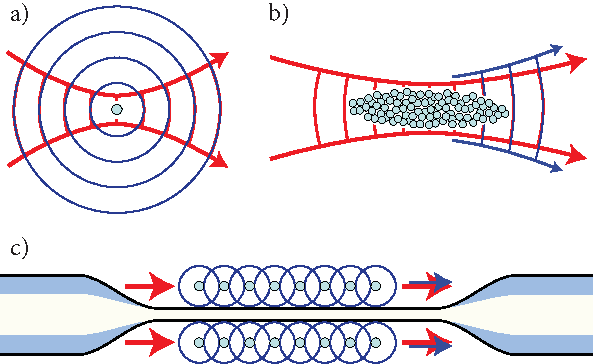
\includegraphics[scale=1.10]{../chap4/Fig1}
\caption[Comparing mode-matching and cooperativity of quantum interfaces in free-space and a nanofiber.]{Cooperativity and mode-matching for various atom-light geometries. (a) The  beam area at the waist of a tightly focused beam is closely matched with the atomic scattering cross section, but the scattered light of a single atom is poorly mode-matched with the probe. (b) A paraxial beam probing a rarefied atomic cloud whose scattered radiation interferes constructively in the forward direction. (c) Atoms trapped in a 1D optical lattices  near the surface of an optical nanofiber interacting with a fiber-guided probe. The tight confinement and automatic mode matching that accompanies scattering into the guided mode leads to strong cooperativity in the atom-photon interaction.}\label{Fig::ModeMatching}
\end{figure}
%=============================================

A particular system that combines the elements above consists of cold atoms trapped in the evanescent field of the guided mode of a tapered optical nanofiber with a subwavelength diameter \cite{vetsch_optical_2010, lacroute_state-insensitive_2012, balykin_quantum_2014, grover_photon-correlation_2015, Lee2015Inhomogeneous} (see \frf{Fig::ModeMatching}).  
The typical resonant OD per atom, or OD/$N_A$, in the nanofiber ($\sigma_0/A \sim  10^{-2}$) is boosted by orders of magnitude over free space for paraxial beams. 
However, one cannot reach the strong coupling regime where $\Gamma_{\oneD}$ is on the order of $\Gamma_{\vac}$ as is possible in engineered nanophotonic waveguides, such as those arising in photonic crystals \cite{hung_trapped_2013}, where atoms can be trapped at positions of peak intensity of the field.  
One can, however, achieve strong cooperativity in the dispersive regime with a moderately sized ensemble.  When compared to free space, all light scattered into the guided mode is automatically mode matched, and thus, given the relatively large ratio $\sigma_0/A$, one can achieve high OD with only a few thousand atoms (see \frf{Fig::ModeMatching}).  
Such strong cooperativity opens the door to new regimes to create non-Gaussian quantum states of the ensemble \cite{dubost_efficient_2012} and potentially to implement nonlinear optics at the level of a few photons \cite{spillane_observation_2008, pittman_ultralow-power_2013, oshea_fiber-optical_2013}.


One-dimensional optical lattices in nanofibers based on multiple co- and counter-propagating trapping beams have been loaded with up to several thousand alkali atoms \cite{vetsch_optical_2010, lacroute_state-insensitive_2012}.
This has proved a fruitful platform for quantum information processing.  
The anisotropic nature of the strong atom-light coupling has been exploited for control of internal atomic states \cite{mitsch_exploiting_2014}, enhanced coupling into a preferred propagation direction \cite{petersen_chiral_2014, mitsch_quantum_2014}, and optical switching \cite{oshea_fiber-optical_2013}. 
Off resonance, dispersive coupling has allowed for non-destructive atom counting \cite{dawkins_dispersive_2011, beguin_generation_2014} 
and storage of fiber-guided light \cite{gouraud_demonstration_2015, sayrin_storage_2015}.
Recent demonstrations of photonic crystal cavities fabricated on the nanofiber \cite{wuttke_nanofiber_2012, nayak_optical_2014, schell_highly_2015} promise further enhanced atom-light coupling.

In this chapter we study the quantum atom-light interface in the dispersive regime for an optical nanofiber geometry.  We focus here on the coupling between the atomic spin and light polarization induced by the elastic scattering of photons by tensor-polarizable cesium atoms trapped near the surface of the nanofiber.  This provides an entangling interaction that can be employed to generate spin squeezing via QND measurement.  Our analysis unifies a variety of different approaches found in the literature, including direct calculation of the dyadic Green's function for photon scattering \cite{Sakoda1996Optical, Dung2000, Sondergaard2001, Klimov2004, Wubs2004, Fussell2005Decay, MangaRao2007Single, dzsotjan_quantum_2010} and the input-output formalism studied for one-dimensional field theories based on Heisenberg-Langevin equations \cite{gardiner_input_1985, blow_continuum_1990, shen_coherent_2005, LeKien2005a, le_kien_correlations_2008, fan_input-output_2010}.

The remainder of this article is organized as follows.  
In \srf{Sec::GreensFunction} we solve for the mode decomposition of the dyadic Green's function which determines the electric field scattered by a point dipole near the surface of the nanofiber.  
This allows us to calculate the phase shift and polarization transformation for fiber-guided photons induced by tensor-polarizable atoms in the dispersive regime.  
We connect this with a fully quantum mechanical treatment based on a Heisenberg-Langevin picture in \srf{Sec::HeisenbergLangevin}.  
The formalism we develop is used in \srf{Sec::QNDMeasurement} to study QND measurement of atoms based on polarization spectroscopy. 
We consider shot-noise-limited atom detection as well as measurement-backaction-induced squeezing of spin projection noise.  
We study squeezing of the collective pseudospin associated with ensembles of atoms in the atomic clock state and calculate its dynamics based on a first principles stochastic master equation that includes both the effects of QND measurement as well as decoherence due to optical pumping.  
We conclude with a summary and outlook for future research in \srf{Sec::Conclusion}.  


%========GREEN'S FUNCTION AND INPUT/OUTPUT RESPONSE=========%
\section{Dyadic Green's function and input-output\\ field response} \label{Sec::GreensFunction}

Given a point particle with tensor polarizability $\tensor{\boldsymbol{\alpha}}$ at position $\br'$ near the surface of a nanofiber, the field  at frequency $\omega_0$ is given by the solution to the wave equation, 
	\begin{align}\label{Eq::WaveEquationSource}
		\left[ - \nabla\times\nabla\times + \, n^2(\br)k_0^2 \right] \mathbf{E}(\br) &= -4\pi  k_0^2 \delta^{(3)}(\br-\br')\,  \tensor{\boldsymbol{\alpha}}\cdot \mathbf{E}(\br),
	\end{align}
where $k_0=\omega_0/c$ and $n(\mbf{r})$ is the spatially varying index of refraction that describes the fiber; Gaussian-cgs units are used throughout.  
For an asymptotic input field $\mathbf{E}_{\inp}(\br)$, the scattering solution to \erf{Eq::WaveEquationSource} is given by the Lippmann-Schwinger equation \cite{Wubs2004},
\begin{subequations}
	\begin{align}
		\mathbf{E}_{\out}(\br) &=\mathbf{E}_{\inp}(\br)+\tensor{\mathbf{G}}^{(+)}(\br , \br'; \omega_0)\cdot 
\tensor{\boldsymbol{\alpha}}\cdot \mathbf{E}_{\out}(\br')\\
		&\approx \mathbf{E}_{\inp}(\br)+ \tensor{\mathbf{G}}^{(+)}(\br , \br'; \omega_0) \cdot 
\tensor{\boldsymbol{\alpha}}\cdot \mathbf{E}_{\inp}(\br'), \label{Eq::ScatteredField}
	\end{align}
\end{subequations}
where in \erf{Eq::ScatteredField} we have made the first Born approximation valid for weak scattering. The fundamental object that fully characterizes the scattered radiation as well as the energy level shift and modified decay rate of a scatterer near the dielectric is the dyadic Green's function, $\tensor{\mathbf{G}}(\br, \br';\omega_0)$. This determines the scattered field from a point dipole at $\br'$, $\mathbf{E}_{\rm scat}(\br)= \tensor{\mathbf{G}}^{(+)}(\br , \br'; \omega_0)\cdot \mathbf{d}$, and satisfies the equation of motion,
	\begin{align} \label{Eq::GreensDiffEq}
		\left[ -\nabla\times\nabla\times + n^2(\mbf{r}) k_0^2 \right] \tensor{\mathbf{G}}(\br, \br';\omega_0) &= -4\pi 
k_0^2 \delta^{(3)}(\mathbf{r}-\mathbf{r}') \unittens,
	\end{align}
where $\unittens$ is the unit tensor.   

The solution for the Green's function $\tensor{\mathbf{G}}(\br ,\br' ; \omega_0)$, following from Maxwell's equations,  
has been studied previously \cite{Sakoda1996Optical,Sondergaard2001,Wubs2004}.
In Chapter 2, we have also derived the eigenmode decomposition solutions for the dyadic Green's function of a nanophotonic waveguide and shown that the radiation modes do not contribute to the sign measured at the end of the waveguide. 
As we are interested here in the forward-scattered components that lead to phase shifts and polarization transformations, we apply the eigenmode decomposition approach derived in Chapter 2 to directly calculate a nanofiber's $\tensor{\mathbf{G}}(\br ,\br' ; \omega_0)$ using the fiber's normal modes and study how the guided modes respond to atoms with a tensor polarizability. 

We treat an optical nanofiber of radius $a$ with step-index profile,
	\begin{align} \label{Eq::IndexofRefraction}
		n(r_\perp) = \Big\{  
			\begin{array}{l l} n_1 & \quad r \leq a \\
						 n_2 & \quad r > a 
		\end{array},
	\end{align}
for a silica core ($n_1 = 1.4469$)~\cite{Kien2004} and infinite vacuum cladding ($n_2 = 1$).  For a cylindrically symmetric dielectric the guided modes are $\mathbf{f}_\mu (\br) = \mathbf{u}_\mu (\br_\perp) e^{i\beta z}/\sqrt{2 \pi}$, with indices $\mu=\{j, \beta , p\}$ for the $j$th guided mode with propagation constant $\beta$ at frequency $\omega_\mu=\omega(\beta)$ and polarization $p$. 
Two convenient guided-mode bases to describe $ \mathbf{u}_\mu (\br_\perp) $ are the quasilinear and quasicircular polarization modes, described in Appendix \ref{chap:fibereigenmodes} \cite{Kien2004}.  

We consider nanofibers that support only the lowest HE$_{11}$ guided modes at the relevant frequency $\omega_0$ \cite{Snyder1983Optical}, which have four guided modes: two polarizations $p$, each with propagation constant $\beta(\omega_0) = \pm\beta_0$ corresponding to forward and backward propagation. We use $ b=\pm $ to indicate the propagation direction. Substituting the guided mode indices into Eq.~\eqref{Eq::GreensGuided_general}, the guided-mode contribution to the dyadic Greens function for $ z\neq z' $ is then 
	\begin{align} 
		\tensor{\mathbf{G}}^{(+)}_g(\br,\br'; \omega_0) = &2\pi i \sum_{b,p}  {\rm Res}\vert_{\beta =b\beta_0} 
\left[\frac{-2 \omega_0^2 }{ \omega_0^2-\omega^2(\beta)}\right]  \mathbf{u}_{b\beta_0, p} 
(\br_\perp)\mathbf{u}^*_{b\beta_0, p} (\br_{\perp}^\prime)e^{ib \beta_0 (z-z')} \nonumber \\
= & 2\pi i \frac{\omega_0}{v_g } \sum_{b,p} \mathbf{u}_{b, p} (\br_\perp)\mathbf{u}^*_{b, p} 
(\br_{\perp}^\prime) e^{i b\beta_0(z-z')} \Theta \big( b(z-z') \big), \label{Eq::GreensGuided}
	\end{align}
where $v_g= \vert d\omega/d\beta \vert_{\beta=\beta_0}$ is the group velocity of the HE$_{11}$ modes at $\omega_0$, and $\Theta \big( b(z-z') \big)$ is a Heaviside function. At $ \br=\br' $, Eq.~\eqref{Eq::ImGreenLocal_general} yields the imaginary part of the dyadic Green's function:
	\begin{equation}\label{Eq::ImGreenLocal}
		{\rm Im} \big[\tensor{\mathbf{G}}^{(+)}_g(\br',\br'; \omega_0=\omega_{eg}) \big] = \pi \frac{\omega_{eg}}{v_g } \sum_{b, p} 
		\mathbf{u}_{b, p} (\br_{\!\perp}^\prime)\mathbf{u}^*_{b , p} (\br_{\!\perp}^\prime),
	\end{equation}
where we have used $\omega_0=\omega_{eg}$ for future calculations of the decay rates of the quantum transitions between the ground state $ \ket{g} $ and the excited state $ \ket{e} $ of the atom.  The real part of the Green's function at $\br = \br'$ determines the energy level shift of the scatterer. 

Equation (\ref{Eq::GreensGuided}) is the central result from which we can calculate the dispersive response.  Consider a forward-propagating input field in the guided modes with frequency $\omega_0$, positive-frequency amplitude $\Eamp$, and arbitrary polarization, $\mathbf{E}^{(+)}_{\inp}(\br) = \Eamp  \mathbf{u}_{\rm in}(\br_\perp) e^{i \beta_0 z}$ dispersively coupled to an atom at position $\mathbf{r}'$.  The effective mode area at the atom's position is determined from the total cycle-averaged power transported along the nanofiber, $P_{{\rm in},z} = (v_g/2\pi) \int d^2\br \, n^2(r_\perp) |\mathbf{E}^{(+)}_{\inp}(\br) |^2$, and the intensity at the atom, $I_{\rm in}(\mathbf{r}') = (c/2\pi) |\mathbf{E}^{(+)}_{\inp}(\br') |^2$, via the relation \cite{domokos_quantum_2002},
 	\begin{align} \label{Eq::AreaIn}
 		A_{\rm in} \equiv \frac{P_{{\rm in}}}{I_{\rm in}(\mathbf{r}')} = \frac{1}{n_g |\mathbf{u}_{\rm in}(\mathbf{r}'_\perp)|^{2}},
	\end{align}
where $n_g\equiv c/v_g$ is the group index of refraction.    

Substitution of the guided-mode Green's function, \erf{Eq::GreensGuided}, into the Lippman-Schwinger equation, \erf{Eq::ScatteredField}, yields the transmitted (forward-scattered) and reflected (backward-scattered) output fields, \begin{equation}
\mathbf{E}_{\out}(\br) = \Eamp \big[ \mathbf{u}_{\trans, \out} (\br_\perp) e^{i \beta_0 z} + \mathbf{u}_{\refl,\out} (\br_\perp) e^{-i \beta_0 z} \big],
\end{equation}
where 
\begin{subequations}
	\begin{align}
		\mathbf{u}_{\trans, \out} (\br_\perp) &=  \sum_{p,p'}  \, c_{p} t_{pp'} \mathbf{u}_{\fwd, p'}(\br_\perp) \\ 
		\mathbf{u}_{\refl,\out} (\br_\perp) &=  \sum_{p,p'}  \, c_{p} r_{pp'} \mathbf{u}_{\bwd, p'}(\br_\perp),
	\end{align}
\end{subequations}
where we have decomposed the input into the polarization eigenmodes, $\mbf{u}_{\rm in}(\mbf{r}_\perp) = \sum_{p} c_{p} \mathbf{u}_{\fwd,p}(\br_\perp)$.  
For $z>z'$, the transmission and reflection matrices are 
\begin{subequations}
	\begin{align} \label{Eq::PolarizationTransformation}
		t_{pp'} =& \delta_{p,p'} +  2\pi i k_0 n_g \, \mathbf{u}^*_{+, p}(\br'_\perp) \cdot 
\tensor{\boldsymbol{\alpha}} \cdot \mathbf{u}_{+, p'}(\br'_\perp) , \\
		r_{pp'} =&  2\pi i k_0 n_g \, \mathbf{u}^*_{\bwd, p}(\br'_\perp) \cdot 
\tensor{\boldsymbol{\alpha}} \cdot \mathbf{u}_{\fwd, p'}(\br'_\perp) e^{2 i\beta_0 z'} , 
	\end{align} 
\end{subequations}
We focus here on the transmitted fields whose interference with the input field for $z>z'$ results in a phase shift and a polarization transformation.  
For weak scattering the diagonal terms, $t_{p p} \approx \sqrt{1-R_p}e^{i \delta \phi_p}$, determine the phase shift and attenuation induced on each polarization mode,
\begin{subequations}
	\begin{align}
		 \delta \phi_p &= \frac{2 \pi k_0}{A_{\rm in}} {\rm Re}(\alpha_{pp}),  \label{Eq::PhaseShift} \\
		R_p &=  \frac{4 \pi k_0}{A_{\rm in}} {\rm Im}(\alpha_{pp}) .\label{Eq::Attenuation} 
	\end{align} 
\end{subequations}
Here, the $\{p,p'\}$-element of the tensor polarizability is given by, $\alpha_{pp'} \equiv \mathbf{e}^*_{p'} \cdot \tensor{\boldsymbol{\alpha}}\cdot \mathbf{e}_{p}$, with unit vectors for each of the forward-propagating mode functions,\linebreak[4] $\mathbf{e}_{p}\equiv \mathbf{u}_{+,p}(\br'_\perp)/|\mathbf{u}_{+,p}(\br'_\perp)|$. 

The phase shift per atom, \erf{Eq::PhaseShift}, is modified over free space in two ways, both of which are captured by the effective mode area $A_{\rm in}$. First, although material dispersion in an optical fiber is negligible over the distances we consider, additional waveguide dispersion can lead to a significant reduction in the group velocity~\cite{hung_trapped_2013,goban_atomlight_2014}.  Such ``slow light" enhances the atom-photon coupling strength. 
In the nanofiber geometry this effect is moderate -- we calculated the group index to be $n_g \approx 1.40$. 
Second and more importantly, the tight spatial confinement as measured by OD/$N_A$ significantly increases the coupling strength over free space for every atom along the nanofiber, which yields strong cooperativity.
In contrast, in free space diffraction restricts the collective phase shift for an ensemble of atoms~\cite{tanji-suzuki_chapter_2011, baragiola_three-dimensional_2014}.  
For a Gaussian beam with beam waist $w_0$, the total phase shift induced by a collection of polarizable atoms will be $\delta \phi = N_{\eff} 2 \pi k_0 {\rm Re}({\alpha})/A$, where $A = \pi w^2_0/2$ is the beam area at the focus and $N_{\eff}$ is the effective number of atoms that radiate into this mode.  
One can couple strongly to few atoms at the center by tightly focusing the beam or couple weakly to many atoms by choosing a larger focal volume, but hence, smaller cooperativity per atom.  

The off-diagonal terms in the transmission matrix, \erf{Eq::PolarizationTransformation}, describe the polarization transformation. For example, if we take the polarization of the modes to be the quasilinear, $p = \{H,V\}$ as defined in \erf{Eq::QuasilinearModes}, then $t_{HV} \equiv \chi_{\rm Far}$ is the rotation angle of the Stokes vector on the Poincar\'{e} sphere corresponding to the Faraday effect \cite{hammerer_quantum_2010, deutsch_quantum_2010}.  
The phase difference in that basis, $\delta  \phi_H - \delta \phi_V$, corresponds to birefringence induced on the guided mode and $t_{HV}$ to Faraday rotation.  
Analyzed in the quasicircular polarization modes ($p=\pm$), given in \erf{Eq::QuasicircularModes}, the differential phase $\delta \phi_+ -\delta  \phi_-$ corresponds to Faraday rotation and $t_{+-}$ to birefringence.  
We make use of such polarization transformations as a means to nondestructively measure the atoms and generate collective spin squeezing.

	
%===================Heisenberg-Langevin Equations=====================%
\section{Heisenberg-Langevin-picture solution\\ and atomic response} \label{Sec::HeisenbergLangevin}
	
The Lippmann-Schwinger solution, \erf{Eq::ScatteredField}, determines the input-output relation for linear atomic response given by the polarizability tensor $\tensor{\alpha}$.  
In this section we connect this with the fully quantum mechanical description of dispersive atomic response and input-output relations for the quantized guided modes.  
Following Ref. \cite{LeKien2005a}, we use a Heisenberg-Langevin approach for one-dimensional systems.  

The positive frequency component of the quantized electric field operator decomposes into guided and radiation (unguided) modes, $\hat{\mathbf{E}}^{(+)}=\hat{\mathbf{E}}_g^{(+)}+\hat{\mathbf{E}}_{r}^{(+)}$, where
\begin{subequations}
	\begin{align}
		\hat{\mathbf{E}}_g^{(+)}(\br) &= \sum_{b,p} \int_0^{\infty}\!\!\!\!\!  \mathrm{d}\omega \sqrt{\frac{ \hbar \omega}{ v_g}} \; \awg \mathbf{u}_\mu (\br\!_\perp) e^{i b\beta(\omega) z } ,\label{Eq::QuantizedElectricField} \\
		\hat{\mathbf{E}}_r^{(+)}(\br) &= \sum_{m,p}\int_0^{\infty}\!\!\!\!\! \mathrm{d}\omega   \int_{-kn_2}^{kn_2}\mathrm{d}\beta \, \sqrt{ \hbar \omega}\;\awr \mathbf{u}_\nu (\br\!_\perp) e^{i\beta(\omega) z }.
	\end{align}
\end{subequations}
The HE$_{11}$ guided modes are specified by $\mu =(\omega, b, p)$, where $\omega$ is the mode frequency,  $p$ is the polarization, and the propagation direction $b=\pm$ corresponds to wavenumber $b \beta (\omega)$.  The radiation modes are specified by  $\nu=(\omega, \beta, m, p)$, where $m$ is the azimuthal (angular momentum) quantum number, $p$ labels the two orthogonal polarizations, and longitudinal propagation constant $\beta$ can vary continuously from $-kn_2$ to $kn_2$, with $k = \omega/c$ \cite{Sondergaard2001,LeKien2005a}.  
The creation/annihilation operators satisfy the usual continuous-mode commutation relations, $[\hat{a}_\mu, \hat{a}^\dag_{\mu'} ] = \delta_{b,b'} \delta_{p,p'} \delta ( \omega - \omega ') $ and $[\hat{a}_\nu ,\hat{a}^\dag_{\nu'} ] = \delta_{m,m'} \delta_{p,p'} \delta ( \omega - \omega ')  \delta ( \beta - \beta') $.

The Hamiltonian for the system is
\begin{equation}
\hat{H} = \hat{H}_F+\hat{H}_A + \hat{H}_{\inter},
\end{equation}
where the free-field Hamiltonian decomposes into guided and unguided modes, 
	\begin{equation}
		\hat{H}_F = \sum_{b,p}\int_0^{\infty}\!\!\!\!\! \mathrm{d}\omega \, \hbar \omega \hat{a}^\dagger_\mu \hat{a}_\mu 
+\sum_{m,p} \int_0^{\infty}\!\!\!\!\! \mathrm{d}\omega  \int_{-k n_2}^{k n_2} \mathrm{d}\beta \, \hbar \omega 
\hat{a}^\dagger_\nu \hat{a}_\nu.
	\end{equation}
We consider here alkali atoms with ground and excited levels, $\{ \ket{g}=\ket{nS_{1/2}, f, m_f}\}$, $\{ \ket{e} =\ket{nP_{j'}, f', m_{f'}}\}$, where $\ket{f, m_f}$ denotes the hyperfine sublevels.  The free atomic Hamiltonian is
	\begin{equation}
		\hat{H}_A  = \sum_g E_g \hat{\sigma}_{gg} + \sum_e E_e \hat{\sigma}_{ee},
	\end{equation}
where $\hat{\sigma}_{ij} \equiv \ket{i}\bra{j}$.  In the rotating wave approximation, the atom-field interaction Hamiltonian is
	\begin{align}
		\hat{H}_{\inter} &= -\hat{\mathbf{d}}\cdot \hat{\mathbf{E}} =- \sum_{e,g} \left[ \hat{\mathbf{d}}_{eg}\cdot 
\hat{\mathbf{E}}^{(+)}(\br')+\hat{\mathbf{d}}_{ge}\cdot \hat{\mathbf{E}}^{(-)}(\br') \right],
	\end{align}
where the atomic dipole operator is projected between excited and ground subspaces, $\hat{\mathbf{d}}_{eg}= \hat{P}_e \hat{\mathbf{d}} \hat{P}_g $. The interaction Hamiltonian then takes the form, 
\begin{equation}
	\hat{H}_{\inter} = -\sum_{e,g} \left(\sum_{b,p} \int_0^{\infty}\!\!\!\!\!\mathrm{d}\omega \; \hbar g_{\mu, e,g}\, \hat{a}_\mu  \, 
		\hat{\sigma}_{eg}+ \sum_{m,p} \int_0^{\infty}\!\!\!\!\!\mathrm{d}\omega \! \int_{-kn_2}^{kn_2}\mathrm{d}\beta \,  \hbar 
g_{\nu, e,g}\, \hat{a}_\nu \, \hat{\sigma}_{eg}\right) + {H.c.},
	\end{equation}
where the coupling constants for guided/radiation modes are
\begin{subequations} \label{Eq::CouplingConstants}
	\begin{align}
		\hbar g_{\mu, e,g} &= \sqrt{\frac{\hbar \omega}{ v_g  }}\, \bra{e} \hat{\mathbf{d}} \ket{g} 
\cdot\mathbf{u}_\mu ( \br'_\perp ) e^{i b \beta(\omega)z} , \\
		\hbar g_{\nu, e,g} &= \sqrt{  \hbar \omega } \, \bra{e} \hat{\mathbf{d}} \ket{g} \cdot \mathbf{u}_\nu ( \br'_\perp) e^{i\beta(\omega)z}  .
	\end{align}
\end{subequations}
The Heisenberg equations of motion are
\begin{subequations}
	\begin{align}
		\der{\hat{a}_\mu} &= -i\omega \hat{a}_\mu +i\sum_{e,g} g_{\mu, e,g}^* \hat{\sigma}_{ge} \label{eq:da},\\
		\der{\hat{a}_\nu} &= -i\omega \hat{a}_\nu +i\sum_{e,g} g_{\nu, e,g}^*  \hat{\sigma}_{ge}\label{eq:danu},\\
		\der{\hat{\sigma}_{ge}} &= -i\omega_{eg} \hat{\sigma}_{ge} \label{Eq::dsigma}  \\
			&+ i\!\int_0^{\infty}\!\!\!\!\! \mathrm{d}\omega \sum_{e',g'} \bigg\{ \big(\delta_{ee'} \hat{\sigma}_{gg'} \!-\! \delta_{gg'} \hat{\sigma}_{e'e} \big) \bigg[ \sum_{b,p}  g_{\mu, e',g'}\hat{a}_\mu \!+\! \sum_{m,p} \!\int_{-kn_2}^{kn_2}\!\!\!\!\!\! \mathrm{d}\beta \; g_{\nu, e',g'} \hat{a}_\nu \bigg] \bigg\}. \nonumber
	\end{align}
\end{subequations}
Integrating the field equations, 
\begin{subequations}\label{eq:aout1}
\begin{align}
\hat{a}_\mu(t) &= \hat{a}_\mu(t_0) e^{-i\omega (t-t_0)} +i \sum_{e,g} g_{\mu,e,g}^* \int_{t_0}^t 
\mathrm{d} t' e^{-i\omega (t-t')}\hat{\sigma}_{ge}(t'), \label{Eq::aguidedEOM}
\end{align}
\begin{align}
\hat{a}_\nu (t) &= \hat{a}_\nu (t_0) e^{-i\omega (t-t_0)} +i \sum_{e,g} g_{\nu,e,g}^* \int_{t_0}^t \mathrm{d} 
t' e^{-i\omega (t-t')}\hat{\sigma}_{ge}(t'),
\end{align}
\end{subequations}
substituting into \erf{Eq::dsigma}, and making the usual Markov\linebreak[4] approximation \cite{LeKien2005a} gives an expression for the ground-excited coherences.   This yields
\begin{align}
&\quad\dt{\hat{\sigma}_{ge}} =-i\omega_{eg} 
\hat{\sigma}_{ge}-\sum_{e'}\frac{\Gamma_{ee'}}{2}\hat{\sigma}_{ge'}  \\
&\!+i\! \sum_{e',g'}\!\!\bigg\{\!\! (\delta_{e,e'} \hat{\sigma}_{\!gg'} \!-\! \delta_{g,g'} 
\hat{\sigma}_{e'e})\!\!\int_0^{\infty}\!\!\!\!\!\!\mathrm{d}\omega \!\bigg[\! \sum_{b,p}  \!g_{\mu, e'\!,g'} \hat{a}_\mu (t_0) 
\!+\!\! \sum_{m,p}\!\!  \int_{-kn_2}^{kn_2}\!\!\!\!\!\!\!\!\!\mathrm{d}\beta  g_{\nu, e'\!,g'} \hat{a}_\nu(t_0) \!\bigg]\! e^{-i\omega 
(t-t_0)}\!\bigg\}\!, \nonumber
\end{align}
where the decay rates of excited-populations and coherences are given by 
	\begin{equation}
		\Gamma_{ee'} = 2\pi \sum_{\mu,g} g_{\mu,e,g}g^*_{\mu,e',g} \vert_{\omega=\omega_{eg}}+2\pi 
\sum_{m,p,g} \int_{-kn_2}^{kn_2}\!\!\!\!\! d\beta \, g_{\nu,e,g}g^*_{\nu,e',g} \vert_{\omega=\omega_{eg}}, \label{Eq::TotaleeDecayRate}
	\end{equation}
and the small energy shift is absorbed into the transition frequency $\omega_{eg} = (E_e - E_g)/\hbar$.  
Equation (\ref{Eq::TotaleeDecayRate}) captures the modification of the spontaneous emission rate due to the nanofiber.  
The first sum describes decay into the guided modes and the second into the unguided radiation modes \cite{ nha_cavity_1997,Klimov2004,LeKien2005a,maslov_distribution_2006, scheel_directional_2015}. The decay rate of a given excited state into all guided modes is given by
	\begin{equation}
		\Gamma_e^{\oneD}= 2\pi \sum_{b,p,g} |g_{\mu,e,g} |^2_{\omega = \omega_{eg}} =  \frac{ 2\pi }{\hbar} \frac{ \omega_{eg} }{v_g} \sum_{b,p,g} \big|\bra{e}\hat{\mathbf{d}}\ket{g} \cdot \mathbf{u}_{bp}(\br'_\perp)\big|^2  .
	\end{equation}
This is in agreement with the expected expression from the guided-mode contribution to the dyadic Green's function in \erf{Eq::ImGreenLocal},
	\begin{equation} \label{Eq::Gamma1DGreens}
		\Gamma_e^{\oneD} =  \frac{2}{\hbar} \sum_{g}  \bra{g}\hat{\mathbf{d}}\ket{e}\cdot 
{\rm Im} \Big[\tensor{\mathbf{G}}^{(+)}_g(\br', \br'; \omega_{eg} ) \Big] \cdot \bra{e}\hat{\mathbf{d}}\ket{g},
	\end{equation}
which is enhanced over the free-space rate by the Purcell factor. 

Here we are interested in linear response for excitation far from resonance. We follow Ref. \cite{le_kien_propagation_2014} and consider an atom sufficiently far from the fiber surface such that the modification of the spontaneous emission rate is small.   In this case the decay rate is approximated as $\Gamma_{ee'} \approx \delta_{e,e'} \Gamma_{e}$, where $\Gamma_e$ is the total decay rate from excited state $\ket{e}$, given by the diagonal elements of \erf{Eq::TotaleeDecayRate}.  In steady state, the dipole operator in the linear regime ($\hat{\sigma}_{ee'} \rightarrow 0 $) is approximately
	\begin{align}
		\hat{\sigma}_{ge} \approx -\sum_{g'} \hat{\sigma}_{gg'}\int_0^{\infty}\mathrm{d}\omega \bigg( & \sum_{b,p}  
\frac{g_{\mu, e,g'}}{\omega-\omega_{eg} + i \Gamma_{e}/2  }\, \hat{a}_\mu (t_0) \\
	&+\sum_{m,p} \int_{-kn_2}^{kn_2}\mathrm{d}\beta \, \frac{g_{\nu, e,g'}}{\omega-\omega_{eg} + i \Gamma_{e}/2 } \,\hat{a}_\nu (t_0)  \bigg)e^{-i\omega (t-t_0)} . \nn
	\end{align}
By substituting this into \erf{Eq::aguidedEOM} and defining asymptotic modes, $\hat{a}^{\inp}(\omega) = \lim_{t_0\rightarrow -\infty} \hat{a}(t_0) e^{i\omega t_0}$, $\hat{a}^{\out}(\omega) = \lim_{t\rightarrow +\infty} \hat{a}(t) e^{i\omega t}$ \cite{fan_input-output_2010}, we obtain the input-output relationship for the guided modes, 
	\begin{align} \label{Eq::aout}
		\hat{a}^{\out}_\mu (\omega) \!= \hat{a}^{\inp}_\mu (\omega) &-\! 2\pi i\sum_{b',p'} 
\sum_{e,g,g'}\!\!\hat{\sigma}_{gg'}\frac{ g_{\mu,e,g}^* g_{\mu'\!\!,e,g'}}{ \omega \!-\! \omega_{eg} \!+\! i \Gamma\!_{e}/2 }\hat{a}^{\inp}_{\mu'}(\omega) \nn\\
&-\! 2\pi i\!\sum_{m\!,p} \sum_{e\!,g\!,g'}\! \int^{kn_2}_{-kn_2}\!\!\!\! \mathrm{d}\beta \,\hat{\sigma}\!_{gg'}\frac{ g_{\mu,e,g}^* g_{\nu'\!\!,e,g'}}{ \omega \!-\! \omega_{eg} \!\!+\! i \Gamma\!_{e}/2 }\hat{a}^{\inp}_{\nu}(\omega).
	\end{align}
	
This input-output relation contains the phase shift on forward scattered modes as well as attenuation due to elastic scattering into all other modes. For a probe with frequency $\omega_0$, \erf{Eq::aout} agrees with the expected form given by the Lippmann-Schwinger equation in the first Born approximation \footnote{In a careful derivation of the Lippman-Schwinger scattering equation, it is not the total Green's function that appears in \erf{Eq::ScatteredField} but rather a related dyadic quantity, $\mbf{K}(\br,\br', \omega_0) = \mbf{G}(\br,\br', \omega_0) + \delta(\br-\br')/n^2(\br)$ \cite{Wubs2004}. 
This function arises by proper accounting of the scatterer's coupling to the \emph{displacement} rather than the electric field \cite{yao_ultrahigh_2009} with a distinction that becomes important at the source point $\mbf{r} = \mbf{r}'$. However, for lossless dielectrics $n(\mathbf{r})$ is real and ${\rm Im}[\tensor{\mathbf{G}}(\br',\br'; \omega)] = {\rm Im}[\tensor{\mathbf{K}}(\br',\br'; \omega)]$ \cite{yao_-chip_2010}. },
	\begin{equation} \label{Eq::IOScatteredField}
		\hat{\mathbf{E}}^{(+)}_{\out,g}(\br, \omega_0)=\hat{\mathbf{E}}^{(+)}_{ \inp, g}(\br, \omega_0)+\tensor{\mathbf{G}}_g^{(+)}(\br,\br', \omega_0)\cdot \poltens \cdot \big[\hat{\mathbf{E}}^{(+)}_{\inp, g}(\br', \omega_0)+\hat{\mathbf{E}}^{(+)}_{\inp,r}(\br', \omega_0) \big],
	\end{equation}
by noting that for the guided-mode dyadic Green's function given in \erf{Eq::GreensGuided},
	\begin{align}
		\int d^2 \mbf{r}_\perp \, \mathbf{u}^*_{\mu} (\br_\perp)\cdot \tensor{\mathbf{G}}_g^{(+)}(\br,\br',\omega_0)\cdot \poltens \cdot \mathbf{u}_{\mu'} (\br'_\perp) &= i \frac{ 2\pi \omega_0}{v_g} \mathbf{u}^*_{b,p} (\br'_\perp) \cdot \poltens \cdot \mathbf{u}_{b'\!\!, p'} (\br'_\perp).  
	\end{align}
Here, the atomic polarizability operator \cite{buhmann_casimir-polder_2004, deutsch_quantum_2010,kien_dynamical_2013}, is given by
	\begin{equation} \label{Eq::PolarizabilityOperator}
		\poltens = - \frac{1}{\hbar} \sum_{e,g,g'}\ket{g}\frac{\bra{g}\hat{\mathbf{d}}\ket{e}\bra{e} 
\hat{\mathbf{d}}\ket{g'}}{\Delta_{eg} + i \Gamma_{e}/2 }\bra{g'},
	\end{equation}	
and $\Delta_{eg} = \omega_0 - \omega_{eg}$ is the laser detuning from the atomic transition.	
For an atom in ground state $\ket{g}$ and polarization $p$, the phase shift can be expressed as \cite{le_kien_propagation_2014}
	\begin{align} \label{Eq::PhaseShiftMultilevel}
		\delta  \phi_{p,g} &=2\pi \frac{ \omega_{0} }{v_g} \mathbf{u}^*_{+, p}(\br'_\perp) \cdot {\rm Re}\big[\bra{g} \hat{\tensor{\boldsymbol{\alpha}}} \ket{g} \big] \cdot \mathbf{u}_{+, p}(\br'_\perp)\nonumber\\
		&= -\frac{ \omega_{0} }{v_g} \sum_e \frac{2 \pi |\bra{e}\hat{\mathbf{d}}\ket{g} \cdot \mathbf{u}_{+,p}(\br'_\perp)|^2}{ \hbar  \Delta_{eg} } .
	\end{align}  
We employ this dispersive response for QND measurement of atoms, as we describe in the next section.



%============== SECITON: QND Measurement ==============%
\section{QND measurement of atoms} \label{Sec::QNDMeasurement}

%========= FIGURE: Geometry (coupling strength, magic wavelength, area and detuning) =========%
\begin{figure}[t]
\centering
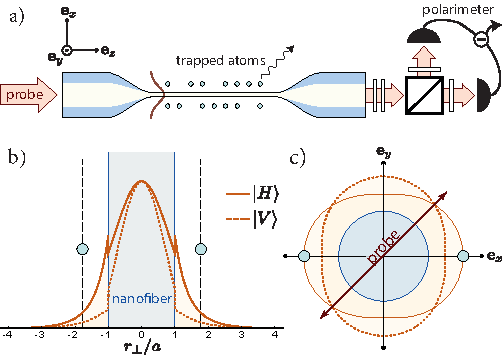
\includegraphics[scale=1.5]{../chap4/Fig2}
\caption[Quantum interface for spin-polarization coupling of two 1D lattices of cold, trapped atoms and the guided modes of an optical nanofiber based on the birefringence effect.]{Quantum interface for spin-polarization coupling of two 1D lattices of cold, trapped atoms and the guided modes of an optical nanofiber. a) Schematic of the interface.  A linearly polarized probe is launched into the nanofiber and the output light is analyzed in a polarimeter.  The atoms (green circles), trapped in the $x$-$z$ plane, couple to the evanescent portion of the guided $H$ and $V$ modes.  Contours of the $H$- and $V$-mode intensities in b) the $x$direction and c) the transverse $xy$ plane show the mode anisotropy at the atomic positions. }\label{Fig::Schematic}
\end{figure}
%=============================================

The dispersive interface between the atoms and nanofiber guided photons provides the entangling mechanism necessary to perform a QND measurement on the atoms.  
We restrict here to the quasilinear modes, $p =\{H,V\}$, of a single HE$_{11}$ guided mode at frequency $\omega_0$, whose form is given explicitly in \erf{Eq::QuasilinearModes}.  
In typical experimental configurations, two one-dimensional arrays of atoms are trapped on either side of the nanofiber, see Fig. \ref{Fig::Schematic}. 
We define coordinate axes $(x,y,z)$ with $z$ oriented along the fiber axis for forward propagation, and the two chains of atoms lie in the $x$-$z$ plane at azimuthal angles $\phi' = \{0, \pi\}$.
In the evanescent region, the $H$ mode is purely $\mathbf{e}_x$-polarized at $\phi = \pm \pi/2$ and the $V$ mode is purely $\mathbf{e}_y$-polarized at $\phi = \{0,\pi\}$.  
At other azimuthal angles the electric field is generally rotating along an ellipse in the $x$-$z$ plane.  The atoms at $\phi'=0$ experience $H$ and $V$ fields,
\begin{subequations}
	\begin{align}
		\mbf{u}_{b,H}(r_\perp, \phi = 0) = & \sqrt{2} \big[ \mathbf{e}_x u_r(r_\perp)+  i b \mathbf{e}_z  u_z(r_\perp) \big] \\
		\mbf{u}_{b,V}(r_\perp, \phi = 0) = & \sqrt{2} \mathbf{e}_y u_\phi(r_\perp), 
	\end{align}
\end{subequations}
where the real-valued functions $u_\alpha(r_\perp)$, given in \erf{Eq::ProfileFunctions}, depend only on the radial coordinate.  
On the opposite side of the fiber at $\phi' = \pi$, atoms experience the same transverse electric field, but the $z$-component changes sign.   This broken symmetry has been used to selectively address and separately control the two atomic arrays \cite{mitsch_exploiting_2014, mitsch_quantum_2014, sayrin_storage_2015}.  

We consider quasi-monochromatic fields at carrier frequency $\omega_0$ that are sufficiently narrowband, $\Delta \omega \ll \omega_0$. 
For each guided mode we define input propagating, continuous-mode field operators in the interaction picture \cite{gardiner_input_1985, blow_continuum_1990, le_kien_correlations_2008},
	\begin{align}
		\hat{a}_{b,p}(z,t) =\frac{1}{\sqrt{2 \pi}}  \int_0^{\infty}\!\!\!\!\! d \omega \, \hat{a}_{b,p}(\omega) e^{i[b \beta_0 z- (\omega-\omega_0) t ]}, 
	\end{align}
that satisfy the free-field commutation relations,
	\begin{equation} \label{Eq::InputOutputCommutation}
		\big[\hat{a}_{b,p}(z,t),\hat{a}^\dag_{b',p'}(z',t')\big]=\delta_{b,b'}\delta_{p,p'}  \delta(t-t'-(z-z')/v_g).
	\end{equation}
In terms of these propagating modes the quantized electric field operator, \erf{Eq::QuantizedElectricField}, becomes
	\begin{equation} \label{Eq::PropagatingElectricField}
		\hat{\mathbf{E}}^{(+)}(r\!_\perp,\phi,z;t) = \sum_{b,p} \sqrt{ \frac{2 \pi \hbar \omega_0}{ v_g} } \mathbf{u}_{b,p}(r\!_\perp,\phi) \hat{a}_{b,p}(z,t)  e^{i b \beta_0 z}.
	\end{equation}	
Considering here only the forward-propagating guided modes ($b=+$), we drop the $b$ index.  
The propagating electric field, \erf{Eq::PropagatingElectricField}, interacts with the trapped atoms via the dispersive light-shift Hamiltonian~\cite{deutsch_quantum_2010,kien_dynamical_2013,baragiola_open_2014},
	\begin{equation} \label{Eq::LightShiftHam}
		\hat{H}_{LS} = - \sum_{n=1}^{N_A} \hat{\mathbf{E}}^{(-)}(\mathbf{r}'_n ; t ) \cdot \poltens {}^{(n)} \cdot \hat{\mathbf{E}}^{(+)}(\mathbf{r}'_n ;t ),
	\end{equation}
where $\poltens {}^{(n)}$ is the atomic tensor polarizability operator, given in \erf{Eq::PolarizabilityOperator}, for the $n^{th}$ atom trapped near the nanofiber surface at position $\mathbf{r}'_n$.  We ignore here any effects of atomic motion and treat the atoms as localized at fixed positions in space.

The Lippmann-Schwinger scattering equation, \erf{Eq::IOScatteredField}, follows in the time domain as the evolution of coarse-grained input-ouput modes \cite{gardiner_input_1985, fan_input-output_2010, le_kien_propagation_2014}.  
Since multiple scattering is negligible and the propagation time across the ensemble is small compared to the atomic dynamics, we drop the position label $z$ and index the propagating fields by time alone; $\hat{a}_{b,p}(z,t) \rightarrow \hat{a}_{b,p}(t) $ as is standard in input-output theory \cite{gardiner_input_1985, stockton_deterministic_2004} . 
It follows that the effects of retardation can be ignored, in which case each term in the sum over atoms contributes equally for all atoms (for details see \cite{le_kien_correlations_2008, baragiola_open_2014}).  
The forward-propagating output fields are then given by the Fourier transform of \erf{Eq::aout}, yielding \cite{le_kien_correlations_2008} 
\begin{align} \label{Eq::ScatteringSolution}
		&\hat{a}^{\rm out}_{p}(t) = \hat{a}^{\rm in}_{p}(t) \nonumber\\
		&+\! i  \frac{2\pi \omega_0}{v_g}\!\sum_{p'}\!\!\Big[\! N_0  \mathbf{u}^*_p(r'_\perp,0) \!\cdot\! \poltens \!\cdot\!  \mathbf{u}_{p'}(r'_\perp,0)  \!+\! N_\pi \mathbf{u}^*_p(r'_\perp,\pi) \!\cdot\! \poltens \!\cdot\!  \mathbf{u}_{p'}(r'_\perp,\pi)\! \Big]\! \hat{a}^{\rm in}_{p'}(t), 
	\end{align} 
where $\{N_0,N_\pi \}$ are the total number of atoms trapped at $\phi' = \{0,\pi\}$. The quantum effects from the first term give rise to shot noise in the transmitted field at the detector.  
The second term represents scattering into the guided modes, as described by the dyadic Green's function, \erf{Eq::Gamma1DGreens}.  

We introduce the vector Stokes operators that describe the polarization of the propagating fields in the quasilinear $HV$-basis,
\begin{subequations}\label{Eq::StokesComponents}
	\begin{align} 
		\hat{S}_1(t) & = \smallfrac{1}{2}\big[ \hat{a}^\dag_H(t) \hat{a}_H(t)-\hat{a}^\dag_V(t) \hat{a}_V(t) \big], \\
	 	\hat{S}_2(t) & = \smallfrac{1}{2}\big[ \hat{a}^\dag_H(t) \hat{a}_V(t)+\hat{a}^\dag_V(t) \hat{a}_H(t) \big], \\ 
		\hat{S}_3(t) & = \smallfrac{1}{2i}\big[ \hat{a}^\dag_H(t) \hat{a}_V(t) -\hat{a}^\dag_V(t) \hat{a}_H(t) \big],
	\end{align}
\end{subequations}
that satisfy equal-$z$ commutation relations following from \erf{Eq::InputOutputCommutation},
	\begin{equation} \label{Eq::StokesCommutation}
		\big[\hat{S}_i(t), \hat{S}_j(t')\big] =i \epsilon_{ijk} \delta(t-t')  \hat{S}_k(t).
	\end{equation}
These, along with the total photon flux operator,
	\begin{equation}
		\hat{S}_0(t) = \smallfrac{1}{2}\big[ \hat{a}^\dag_H(t) \hat{a}_H(t)+\hat{a}^\dag_V(t) \hat{a}_V(t) \big],
	\end{equation}
are used to reexpress the Hamiltonian, \erf{Eq::LightShiftHam}, in the $HV$-basis,
	\begin{align}  
		\hat{H}_{LS} 	=& - 2 \pi \hbar k_0 n_g \nonumber \\
		&\times\!\sum_{\phi'=0,\pi}N_{\phi'} \Big\{ \big[ \polcomp_{HH}(\phi')+\polcomp_{VV}(\phi') \big] \hat{S}_0(t) +  \big[\polcomp_{HH}(\phi')  - \polcomp_{VV}(\phi')  \big] \hat{S}_1(t)  \nonumber  \\
&\quad\quad +\! \big[\!\polcomp_{HV}(\phi') \!+\! \polcomp_{VH}(\phi')  \!\big] \hat{S}_2(t) \!+\! i  \big[\! \polcomp_{HV}(\phi')\!-\!\polcomp_{VH}(\phi') \big]\hat{S}_3(t) \Big\}. \label{Eq::GenHamiltonian}
	\end{align}
The atomic couplings to the $\{H,V\}$ modes,
	\begin{align} 
		\polcomp_{p p'}(\phi') & \equiv |\mathbf{u}^*_p(r'_\perp, \phi')||\mathbf{u}_{p'}(r'_\perp, \phi')| \, \hat{\alpha}_{p p'}(\phi') , 
	\end{align}
are determined by components of the quantum mechanical tensor operator weighted by the transverse mode functions at the atomic position, $\hat{\alpha}_{p p'}(\phi') = \mathbf{e}^*_{p'}(\phi') \cdot \poltens \cdot \mathbf{e}_{p}(\phi') $, whose classical analog appeared in \erf{Eq::PhaseShift}.

We explore a QND measurement of ${}^{133}$Cs atoms in the electronic ground state, $6S_{1/2}$, via polarization spectroscopy based on the collective atom-light coupling described by the dispersive light-shift Hamiltonian in \erf{Eq::GenHamiltonian}. Polarization transformations occur due to the tensor nature of the atomic response,
	\begin{align} \label{Eq::Polarizability}
		\poltens &=  \sum_{f,f'} \charpol \sum_{i,j} \hat{\tensor{\mbf{A}}}(f,f'),
	\end{align}
where the operator $\hat{\tensor{\mbf{A}}}(f,f') = \sum_{i,j} \hat{A}_{ij}(f,f')\mathbf{e}_i \otimes \mathbf{e}_j$ decomposes into irreducible components within each ground hyperfine multiplet $f$ for light detuned near excited multiplet $f'$,  
	\begin{align} \label{Eq::PolarizabilityIrrep}
		\hat{A}_{ij}(f,f')&=  C_{ff'}^{(0)} \delta_{i,j}+ iC_{ff'}^{(1)}\epsilon_{ijk}\hat{f}_k+ C_{ff'}^{(2)} \Big[ \smallfrac{1}{2} ( \hat{f}_i\hat{f}_j +\hat{f}_j\hat{f}_i )-\smallfrac{1}{3} \hat{\mathbf{f}}\!\cdot\!\hat{\mathbf{f}} \delta_{i,j} \Big]. 
\end{align}
Here, $\charpol = -\frac{\sigma_0}{8\pi k_0}\frac{\Gamma }{\Delta_{ff'}+i\Gamma/2}$ is the characteristic dynamic polarizability where $\sigma_0 = 3 \lambda^2/2\pi$ is the resonant scattering cross section, $\hat{\mathbf{f}}$ is the atomic  spin operator in hyperfine multiplet $f$, and $C_{ff'}^{(K)}$ are coefficients for irreducible rank-$K$ components defined in \cite{deutsch_quantum_2010}. 

In addition to the atomic tensor response, the nanofiber geometry gives rise to unique features of polarization spectroscopy not present in free space.  The spatial anisotropy of the intensity for the quasilinearly polarized guided modes leads to unequal scattering of the $H$ and $V$ modes, producing \emph{intrinsic} birefringence even for a purely scalar atomic polarizability.  
In particular, atoms trapped on the quasi-$H$ axis leads to a phase delay of this mode relative to the fast quasi-$V$ axis. 
This birefringence was exploited by Dawkins {\em et al.} \cite{dawkins_dispersive_2011} as a mechanism for implementing a dispersive QND measurement of the number of atoms trapped around the nanofiber, as we treat in the next section. 


	%=================== Atom number measurement =====================%
	\subsection{Dispersive atom number measurement} \label{Sec::AtomNumberMeasurement}

The anisotropy of the guided modes provides a mechanism for counting the number of atoms trapped around the nanofiber based on polarization spectroscopy.  
We consider $N_A$ atoms, each in a completely mixed hyperfine spin state. In this case the atomic polarizability tensor in \erf{Eq::PolarizabilityIrrep} reduces to $\langle \hat{A}_{ij}(f,f') \rangle = C_{ff'}^{(0)} \delta_{i,j}$, and the collective interaction is determined entirely by the the scalar (rank-0) terms.  
With the atoms trapped along the quasi-$H$ axis, while $\expt{ \polcomp_{HH} } \neq  \expt{ \polcomp_{VV} }$, the off-diagonal elements in \erf{Eq::GenHamiltonian} do not contribute to the Birefringent interaction we are interested in and actually vanish ($\expt{ \polcomp_{HV} } = \expt{ \polcomp_{VH} } =0$) when $x-$, $ y- $ or $ z- $axis is chosen as the quantization axis which includes the one close to the optimal choice of quantization axis for spin squeezing we will discuss in the next section.  
Atoms on either side of the nanofiber experience the same scalar light shift yielding from  \erf{Eq::GenHamiltonian} the Hamiltonian for QND measurement of atom number,
	\begin{align}
		\hat{H}_{N} =& -2\pi \hbar k_0 n_g \sum_{\phi' = \{0,\pi \}} N_{\phi'} \big[ \expt{ \polcomp_{HH}(\phi')}  - \expt{ \polcomp_{VV}(\phi')} \big] \hat{S}_1(t)  \nonumber \\
		& =  \hbar \chiN N_A \hat{S}_1(t).  \label{Eq::MixedHamiltonian}
	\end{align}	
This birefringent interaction induces a rotation of the Stokes vector  around the $S_1$ axis on the Poincar\'{e} sphere through an angle, 
	\begin{equation} \label{Eq::RotationAngle}
		\chiN = \frac{\sigma_0}{\Abir}  \sum_{f,f'}  C_{ff'}^{(0)} \frac{\Gamma}{2 \Delta_{ff'}},
	\end{equation}
characterized by an effective area, $\Abir^{-1} \equiv (n_g/2) \big[ |\mathbf{u}_{H}(\br'_\perp)|^2 - |\mathbf{u}_{V}(\br'_\perp)| ^2 \big]$. In this case, the polarizability of the atom can be treated as a scalar, since the atoms do not have a preferred state of photons to emit. Therefore, Eq.~\ref{eq:birefringencerotang} characterizes the rotation angle of the polarization state of the light, $ \varphi $, on the \Poincare sphere due to the interaction with one atom. With $ N_A $ atoms, the total rotation angle of the light on the \Poincare sphere is proportional to $ \varphi_N=N_A\varphi $, scaled by the power of the input light. 

Dawkins {\em et al.} \cite{dawkins_dispersive_2011} used this interaction to make a dispersive measurement of $N_A$ via birefringence polarimetry in the usual way: launching linearly polarized light at 45$^\circ$ to the quasi-$H$ axis, $\mbf{u}_\inp = (\mbf{u}_H + \mbf{u}_V )/\sqrt{2}$, and measuring the differential power between the guided right-and left-circularly polarized photons. 
Thus, the integrated measurement is described by the operator $\hat{\mathcal{M}} \equiv \int_0^T dt' \hat{S}^{\rm out}_3(t').$  The shot-noise variance of the polarimeter, $\shotnoise =  \chiN^2 \dot{N}_L T$ for integration time $T$,  determines the fundamental resolution of the polarimeter.  
The smallest detectable atom number using this dispersive measurement is thus, $\delta N_A \sim ( \chiN^2 \dot{N}_L T)^{-1/2}$ \cite{smith_faraday_2003}. We provide the detailed analysis in Appendix~\ref{sec:birefringenceresolution}. 
In an ideal setting, $\delta N_A$ can always be reduced by increasing the integration time, but in practice this time is limited by atom loss. As a coarse approximation we take this time to be $T=\gamma_s^{-1}$, where $\gamma_s$ is the photon scattering rate in free space, and assume perfect quantum efficiency of the detectors.  
For detuning $\Delta$ large compared to the excited hyperfine splitting on the D1- or D2-line ($j' = 1/2$ or $3/2$), the unit-oscillator scattering rate is 
$\gamma_s =\frac{\sigma_0}{A_{\rm in}}\left(\frac{\Gamma}{2 \Delta}\right)^2 \dot{N}_L $, 
with effective area determined by the probe at the atomic position, \erf{Eq::AreaIn}.  
In this limit, the rotation angle $\chiN = C^{(0)}_{j'} (\sigma_0/\Abir)(\Gamma/2\Delta)$, \erf{Eq::RotationAngle}, yields a shot noise-limited atom number resolution, 
	\begin{align} \label{Eq::AtomNumberResolution}
		\delta N_A  &\sim \frac{1}{C^{(0)}_{j'}}\sqrt {\frac{\Abir^2}{A_{\rm in} \sigma_0}},
	\end{align}
where $ C^{(0)}_{j'}=\sum_{f,f'}C^{(0)}_{ff'}$ are the far-detuned, rank-$0$ coefficients on a $j \rightarrow j'$ transition \cite{deutsch_quantum_2010}.  
Using the parameters reported by Dawkins \emph{et al.}~\cite{dawkins_dispersive_2011}, we find the shot-noise limited minimum detectable atom-number $\delta N_A \sim 10$ for atoms trapped at $ 1.8a\sim 2.0a $ from the fiber axis with a D2-line probe light. We plot the estimation result in Fig.~\ref{fig:AminNA_D12_n1d4469_a225nm_rp}.

\begin{figure}
\begin{minipage}{.48\linewidth}
\centering
\subfloat[]{\label{fig:deltaNA_D12_n1d4469_a225nm_rp}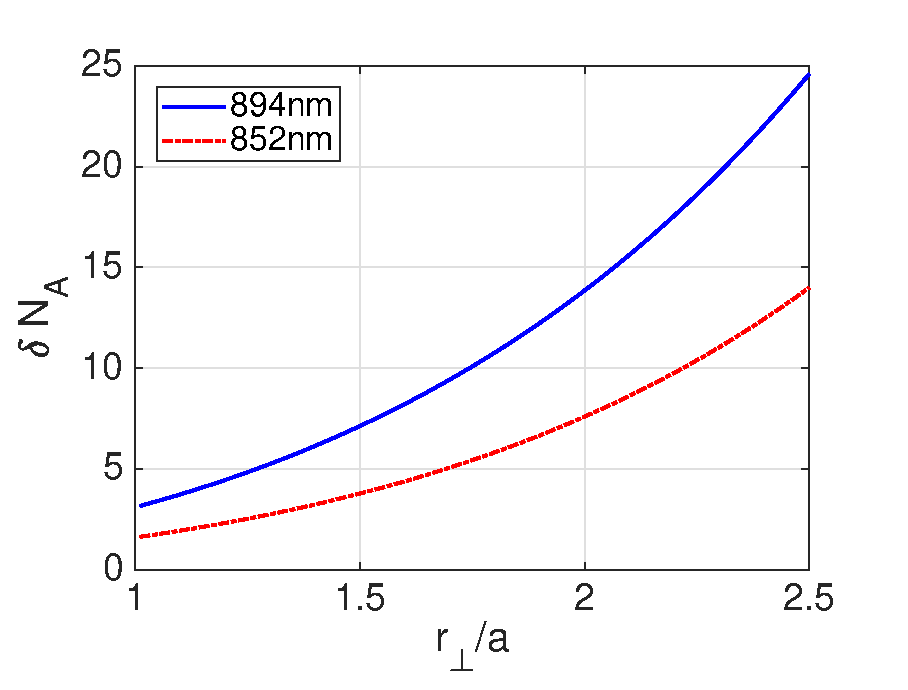
\includegraphics[scale=0.45]{../media/Figs/deltaNA_D12_r1to2d5a}}
\end{minipage}
\begin{minipage}{.48\linewidth}
\centering
\subfloat[]{\label{fig:A_D12_n1d4469_a225nm_rp}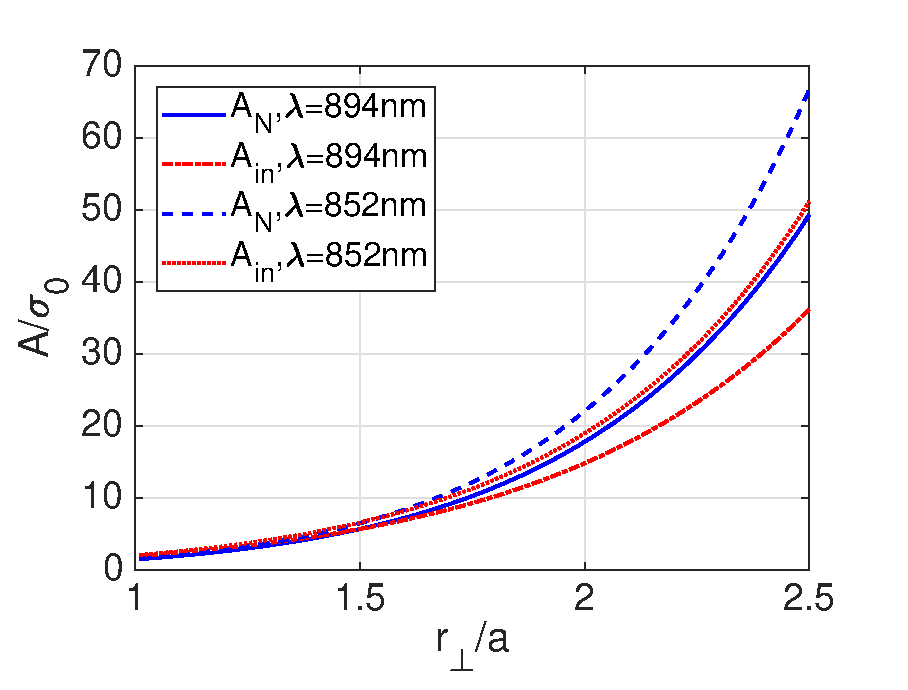
\includegraphics[scale=0.45]{../media/Figs/ANAin_D12_r1to2d5a}}
\end{minipage}
\caption[Minimum detectable atom number and mode areas as functions of the atom radial position, $ r\!_\perp/a $, when the D1- and D2-line probe lasers are used.]{Minimum detectable atom number (a) and mode areas (b) as functions of the atom radial position, $ r\!_\perp/a $, when the D1- and D2-line probe lasers are used. The group indices of refraction are $ n_g=1.4737 $ and $ n_g=1.4974 $ for the D1 ($ \lambda=894 $ nm) and D2 ($ \lambda=952 $ nm) lines, respectively. }\label{fig:AminNA_D12_n1d4469_a225nm_rp}
\end{figure}

In practice, loss and decoherence limit the atom-number resolution~\cite{dawkins_dispersive_2011, zhang_collective_2012}. 
The experimental implementation reported by Dawkins \emph{et al.}~\cite{dawkins_dispersive_2011} implies a resolution of a few tens of atoms for $ 200\sim 1000 $ trapped atoms.  
A similar experiment based on a two-color QND measurement in a nanofiber geometry was recently carried out by \emph{B\'{e}guin et al.} \cite{beguin_generation_2014} to squeeze the uncertainty in the number of trapped atoms. They achieved an atom number uncertainty of $\delta N_A = 8$ for $N_A\sim2500$ atoms, well below standard quantum limit, $\delta N_A=\sqrt{N_A}$.



	%===================QND spin squeezing=====================%
	\subsection{Collective spin squeezing via QND measurement}

The same birefringent interaction, \erf{Eq::GenHamiltonian}, can be utilized in a QND measurement to squeeze the projection noise of the collective atomic spin.  We consider squeezing of the uncertainty associated with the ``clock states" of cesium\index{state!clock state}, $\ket{\uparrow} = \ket{6S_{1/2}, f=4, m_f=0}$ and $\ket{\downarrow} = \ket{6S_{1/2}, f=3, m_f=0}$, which define a pseudospin within each atom and associated Pauli operators $\{\hat{\sigma}_x, \hat{\sigma}_y, \hat{\sigma}_z\}$.  The quantum uncertainty in the collective pseudospin,
	\begin{align}
		\jz = \frac{1}{2} \sum_{n=1}^{N_A} \hat{\sigma}_z^{(n)},  
	\end{align}
fundamentally limits the precision of atomic clocks \cite{wineland_spin_1992}. For atoms prepared in a spin coherent state (SCS) the projection noise, $\varz \big|_{\scs} = N_A/4$, sets the standard quantum limit for spin measurements. A spin squeezed state (SSS) exhibits reduced fluctuations, $ \varz \big|_{\rm SSS}  < N_A/4$, due to negative pairwise correlations between the atoms \cite{kitagawa_squeezed_1993}. Spin squeezing is typically quantified with the metrological squeezing parameter defined by Wineland \emph{et al.} \cite{wineland_spin_1992},
	\begin{align} \label{Eq::SqueezingParameter}
		\xi^2 \equiv N_A \frac{ \varz }{ \expt{\hat{J}_{||}}^2 },
	\end{align}
where $\expt{\hat{J}_{||}}$ is the mean collective spin along the direction of spin polarization. 

The clock states\index{state!clock state} are defined to have zero projection of angular momentum with respect to a bias magnetic field that defines a quantization axis, $\mathbf{e}_{\tilde{z}}$.  
Within the clock-state subspace the rank-1 vector light shift in the dispersive Hamiltonian, \erf{Eq::GenHamiltonian}, vanishes since $\bra{\uparrow}\hat{f}_k \ket{\uparrow} =\bra{\downarrow}\hat{f}_k \ket{\downarrow} = 0$ for any direction of the spin, $k$, and any quantization axis, $\mathbf{e}_{\tilde{z}}$. 
Furthermore, as shown below, atoms on either side of the nanofiber experience the same birefringent coupling. 
The resulting Hamiltonian, restricted to the clock subspace, couples the guided field of the nanofiber to the $J_z$-component of the collective pseudospin. The interaction has contributions from both the scalar and tensor light shifts,
	\begin{align} \label{Eq::ClockHamiltonian}
		\hat{H}_{J_z} = \hbar \Big\{ & \big[ \big( \chi_{H,\uparrow} +\chi_{V,\uparrow} \big) - \big( \chi_{H,\downarrow} + \chi_{V,\downarrow}\big) \big] \jz \hat{S}_0(t) \\
		+ & \big[  \big( \chi_{H, \uparrow} - \chi_{V,\uparrow} \big) - \big(\chi_{H,\downarrow} - \chi_{V,\downarrow} \big) \big]  \jz \hat{S}_1(t) \Big\}, \nonumber
	\end{align}
where the coupling strength between an atom in the clock subspace and a photon with polarization $p = \{H,V\}$ is
	\begin{equation} \label{Eq::ClockCouplingStrength}
		\chi_{p,f} \equiv - 2\pi k_0 n_g  | \mathbf{u}_p(\mbf{r}_\perp)|^2 \bra{f,0}\hat{\alpha}_{pp}  \ket{f,0},
	\end{equation}
and $f = \{4,3\}$ labels $\{\uparrow,\downarrow\}$.  
The diagonal terms in the polarizability tensor are the same for atoms at positions above and below the nanofiber, and thus all atoms contribute equally. 
In addition, a constant birefringence proportional to $ \hat{J}_0\hat{S}_1 $ is neglected here as it can be canceled with a compensating waveplate. 
Finally, the first term in \erf{Eq::ClockHamiltonian} does not affect polarization spectroscopy, but will act to rotate the pseudo-spin around the $J_z$ axis of the generalized Bloch sphere proportional to classical intensity fluctuations.
While this does not affect the squeezing of projection noise in $\hat{J}_z$, it affects the metrologically relevant squeezing by adding uncertainty to the direction of the mean spin.  By choosing a ``magic frequency" at which the light shifts on the two clock states\index{state!clock state} are equal, 
	\begin{align} \label{Eq::MagicWavelengthCondition}
		\chi_{H,\uparrow} +\chi_{V,\uparrow}  = \chi_{H,\downarrow} + \chi_{V,\downarrow},
	\end{align}
this term can be canceled \cite{chaudhury_continuous_2006}, where we have ignored the imaginary part of the coupling strengths in the dispersive regime.
Using the D1-line of $^{133}$Cs atoms as the probe light, there are two magic-frequency solutions, $ \magic{3} $ and $\magic{4}$, shown in \frf{Fig::CouplingStrength}(a).  

Because the guided probe light at the position of the atom will generally be elliptical, the light-shift interaction coherently couples different magnetic sublevels in a given manifold $f$, and thus does not conserve $\hat{J}_z$.  For example, the ellipticity of the probe light leads to a fictitious magnetic field proportional to $i \mathbf{E}^{(-)}_{\inp}(\br') \times \mathbf{E}^{(+)}_{\inp}(\br')$ that causes a precession of the spin within hyperfine manifold $f$.  This can be mitigated by a sufficiently strong bias magnetic field compared to the fictitious field \cite{smith_continuous_2004}. 


%========= FIGURE: Geometry (coupling strength, magic wavelength, area and detuning) =========%
\begin{figure}[!htbp]
\centering
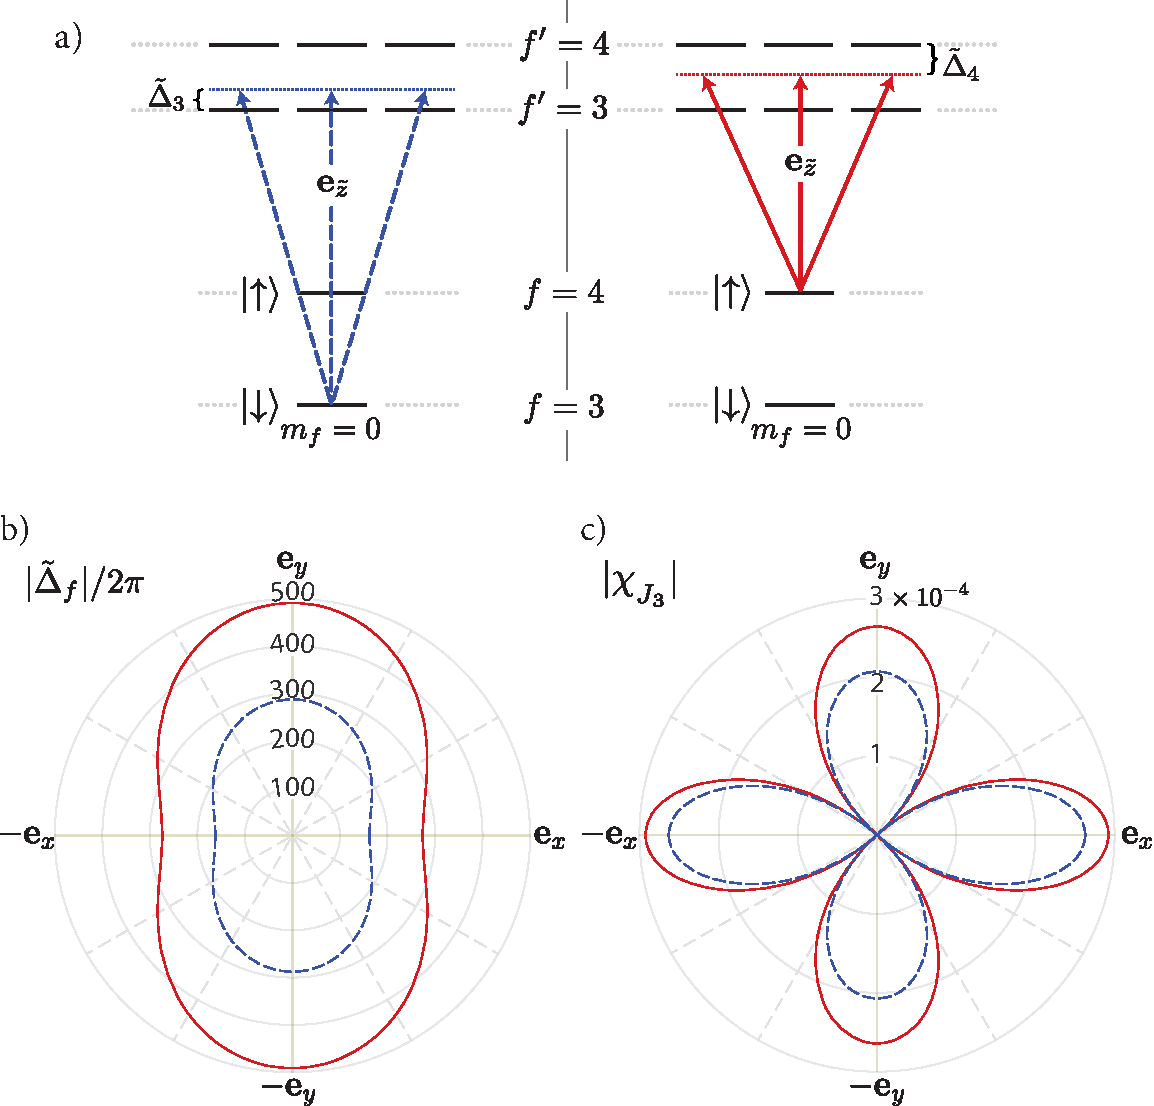
\includegraphics[scale=0.64]{../chap4/Fig3}
\caption[Parameters of the atom-light interface using the clock states of $^{133}$Cs and magic frequencies.]{Parameters of the atom-light interface using the clock states of $^{133}$Cs.  
(a) Energy level structure for atoms probed with one of two magic frequencies on the D1-line. 
(b) Magnitude of the magic detunings at which the clock states are equally light-shifted, $| \tilde{\Delta}_{f}|/2\pi \equiv | \omega_0 - \magic{f} |/2\pi$ (in units of MHz). There are two solutions shown as blue (dashed) and red lines. (c) The coupling strength, as measured by the magnitude of the polarization rotation angle on the Poincar\'{e} sphere, $|\chi_{_{ J_z}}|$, for an atom trapped in the $x$-$z$ plane at a distance $ r'\!_\perp=1.8a $ from the fiber center.  In both (b) and (c) we plot the parameter as the direction of the clock-state quantization axis is varied in the $x$-$y$ plane, for the two possible choices of magic detunings.
See text for details.}\label{Fig::CouplingStrength}
\end{figure}
%=============================================


The remaining QND interaction Hamiltonian is
	\begin{equation} \label{Eq::FaradayHam}
		\hat{H}_{J_z} = \hbar \chieff \jz \hat{S}_1(t),
	\end{equation}
where the rotation angle on the Poincar\'{e} sphere at the magic wavelength is,
\begin{equation}\label{eq:chiJ3}
\chieff = \big( \chi_{H, \uparrow} - \chi_{V,\uparrow} \big) - \big(\chi_{H,\downarrow} - \chi_{V,\downarrow} \big) = 2(\chi_{H, \uparrow}-\chi_{H, \downarrow}).
\end{equation}
In the standard way, squeezing the uncertainty in $\jz$ by QND measurement can be generated by preparing the atoms in a SCS along $\jx$, passing a probe prepared along $\hat{S}_2$ with photon flux $\dot{N}_L$, and continuously monitoring the $S_3$-component of the guided light in a polarimeter. The measurement strength,
	\begin{align} \label{Eq::MeasurementStrength}
		\kappa \equiv |\chieff|^2 \dot{N}_L, 
	\end{align}
quantifies the rate at which we squeeze projection noise, with $\chieff$ given in \erf{eq:chiJ3}. 
In the absence of any decoherence, such a QND measurement for integration time $T$ squeezes the initial uncertainty in $\jz$ according to $(\Delta J_z^2)_{\rm out}= (\Delta J_z^2)_{\rm in}/(1+r)$, where
	\begin{equation}
		r = \kappa T  (\Delta J_z^2)_{\inp}
	\end{equation}
is the integrated measurement strength \cite{hammerer_quantum_2010, baragiola_three-dimensional_2014}.

The strength of the birefringent interaction arises from two fundamental sources.  The anisotropy of the   $H$ and $V$ polarized modes leads to a polarization-dependent index of refraction, as described in Sec.~\ref{Sec::AtomNumberMeasurement}.  In addition there is a dependence of the atom-photon coupling on the internal spin state of the atom due to the atomic tensor polarizability.  In particular, we are interested in the dependence on the two clock states of the atom.  This spin-dependent coupling will depend on the choice of quantization axis that defines the clock state\index{state!clock state} with projection $m_f=0$. 

We combine these two effects and obtain a compact expression for the coupling strength $\chieff$ using the irreducible tensor decomposition of the atomic polarizability, \erf{Eq::PolarizabilityIrrep}.  
Let $\{\mathbf{e}_{\tilde{x}},\mathbf{e}_{\tilde{y}}, \mathbf{e}_{\tilde{z}}\}$ be a space-fixed Cartesian coordinate system, where $\mathbf{e}_{\tilde{z}}$ defines the quantization axis of the atom, set by the magnetic field.  Because of the azimuthal symmetry of clock state around the $\qaxis$ axis, the polarizability tensor is diagonal in that basis.  
Noting that $\langle f,0 | \hat{f}_{\tilde{z}}| f,0 \rangle =0$ and $\langle f,0 | \hat{f}_{\tilde{x}}^2| f,0 \rangle = \langle f,0 | \hat{f}_{\tilde{y}}^2| f,0 \rangle = \langle f,0 | \hat{\mathbf{f}}^2| f,0 \rangle /2 =f(f+1)/2$, it follows that the expectation value of the irreducible rank-2 component of the atomic polarizability is
	\begin{align} \label{Eq::CouplingAngleMagic}
		\langle f,0 | \poltens \phantom{}^{(2)}| f,0 \rangle = \sum_{f'} \charpol C^{(2)}_{ff'} \frac{f(f+1)}{6} \Big( \unittens - 3\qaxis \otimes \qaxis \Big).
	\end{align}
The combined scalar and tensor light shifts yield a coupling strength, \erf{Eq::ClockCouplingStrength},
	\begin{align}
		\chi_{p,f} &  = n_g \sigma_0 \big(  a_{f} \left|\mathbf{u}_p(\br'_\perp)\right|^2 - b_{f} \left|\mathbf{e}_{\tilde{z}} \cdot \mathbf{u}_p(\br'_\perp)\right|^2 \big), \label{Eq::ClockStateCoupling}
	\end{align}
with coefficients that depend on detunings and atomic structure,
	\begin{align}
		a_f &= \sum_{f'}  \Big(C^{(0)}_{ff'} + \frac{f(f+1)}{6} C^{(2)}_{ff'} \Big) \frac{\Gamma}{4 \Delta_{ff'}},\\
		b_f &= \frac{f(f+1)}{2}\sum_{f'} C^{(2)}_{ff'}  \frac{\Gamma}{4 \Delta_{ff'}}.
	\end{align}
At the magic wavelength set by \erf{Eq::MagicWavelengthCondition},
\begin{equation}
	\frac{a_4-a_3}{b_4-b_3} =  \frac{ |\mathbf{e}_{\tilde{z}} \cdot \mathbf{u}_V(\br'_\perp)|^2  + |\mathbf{e}_{\tilde{z}} \cdot \mathbf{u}_H(\br'_\perp) |^2 }{ |\mathbf{u}_H(\br'_\perp)|^2 + |\mathbf{u}_V(\br'_\perp)|^2 },
\end{equation}
which depends on the choice of quantization axis. Note that, in Appendix~\ref{chap:magicwavelength}, we prove the magic wavelengths can be found only if we utilize the tensor polarizability of atoms and design some multi-color schemes for the QND measurement and spin squeezing. We will not discuss the details in the main text here.

We write the effective rotation angle in the Hamiltonian, \erf{Eq::FaradayHam}, as
	\begin{align} \label{Eq::chieff}
		\chieff = \frac{\sigma_0}{A_{J_z}} \frac{\Gamma}{ 2 \Delta_{J_z}},
	\end{align}
with an ``effective detuning" set by the magic-wavelength condition,
	\begin{align} \label{Eq::SqueezingEffectiveDetuning}
		 \Delta_{J_z}^{-1} \equiv \frac{4}{\Gamma} (b_4 - b_3) =   \sum_{f'}  \left( C^{(2)}_{4f'}\frac{10}{\Delta_{4f'}} -  C^{(2)}_{3f'}\frac{6}{ \Delta_{3f'} } \right),
	\end{align}
and an effective area given by
	\begin{align} \label{Eq::SqueezingModeArea}
		A_{J_z}^{-1} & = n_g \frac{ |\mathbf{e}_{\tilde{z}} \cdot \mathbf{u}_V(\br'_\perp)|^2 |\mathbf{u}_H(\br'_\perp)|^2 - |\mathbf{e}_{\tilde{z}} \cdot \mathbf{u}_H(\br'_\perp) |^2 |\mathbf{u}_V(\br'_\perp)|^2 }{ |\mathbf{u}_H(\br'_\perp)|^2 + |\mathbf{u}_V(\br'_\perp)|^2 } 
	\end{align}	
We see here the explicit dependence of the coupling strength on both the anisotropy of the modes and on the tensor atomic response, which in turn depends on a particular choice of clock states\index{state!clock state}.  The quantization axis that maximizes $\chieff$ is that which minimizes $A_{J_z}$ at a given magic detuning.  
Since the $z$-component of the guided modes is $90^\circ$ out-of-phase with the transverse components, the quantization axis maximizing the atom-light coupling is specified by an angle in the transverse $x$-$y$ plane, $\varphi$,
	\begin{align} \label{Eq::QuantizationAxis}
		\qaxis = \cos \varphi \mbf{e}_x + \sin \varphi \mbf{e}_y.
	\end{align}
The dependence of the magic detunings on the direction of quantization axis is shown in \frf{Fig::CouplingStrength}(b) for atoms trapped at a typical distance of $r_\perp'=1.8a$ on the $x$ axis.   
In typical operating regimes, the magic frequencies are hundreds of MHz from resonance with either excited state, placing the interaction in the off-resonant, dispersive regime.  
Using these magic detunings, in \frf{Fig::CouplingStrength}(c) we show the variation in $\chieff$ as a function of $\varphi$.  
This suggests that, based solely on the strength of the coherent interaction, the $x$ axis is the optimal quantization axis. 
As we will see in the next section, the optimal quantization axis is significantly modified when decoherence due to optimal pumping is included.


	%====== SUBSECTION: Including optical pumping ======%
	\subsection{Decoherence due to optical pumping}\label{sec:decoherence}
	
The treatment above considers an idealized QND interaction. 
The coupling of the atoms to the probe, however, will always lead to scattering of photons into modes other than the forward-scattered guided mode.  
This is accompanied by optical pumping that destroys the entanglement associated with spin squeezing.  In addition it reduces the metrologically useful signal.  
The maximum achievable metrologically relevant squeezing is determined by the balance of this decoherence with the QND measurement. 

We model this using a first-principles stochastic master equation description (SME)~\cite{jacobs_straightforward_2006, baragiola_three-dimensional_2014},
	\begin{align} \label{Eq::SME}
		d \hat{\rho} = s\sqrt{\frac{\kappa}{4}} \mathcal{H}[\hat{\rho}] dW + \frac{\kappa}{4} \mathcal{L}[\hat{\rho}] dt + \sum_n \mathcal{D}_n [\hat{\rho}] dt,
	\end{align}
where $s = {\rm sign}(\chieff)$ and $\hat{\rho}$ is the collective atomic state. 
The measurement strength $\kappa =|\chieff|^2 \dot{N}_L$ determines the rate of the spin squeezing in the absence of decoherence.  
The first two terms describe the QND measurement, where $dW$ is a stochastic Weiner increment satisfying $dW^2 = dt$. 
The conditional dynamics that result from the measurement are generated by the superoperator
	\begin{align}
		\mathcal{H}[\hat{\rho}] = \jz \hat{\rho} + \hat{\rho} \jz - 2 \expt{\jz} \hat{\rho},
	\end{align}
and the collective Lindblad map is
	\begin{align}
		\mathcal{L}[\hat{\rho}] = - \smallfrac{1}{2} \big( \hat{\rho}  \jz^2 + \jz^2 \hat{\rho} \big) + \jz \hat{\rho} \jz.
	\end{align}
The final term in \erf{Eq::SME} describes the effect of optical pumping acting locally on each atom along the nanofiber. 

The optical pumping map is governed by a standard master equation~\cite{deutsch_quantum_2010}.  
Restricting to the two-dimensional subspace associated with the clock states\index{state!clock state}, the action on the $n^{th}$ atom is
	\begin{align}
		\mathcal{D}_n[\hat{\rho}] =  \sum_{f=3,4} \Big\{& -\frac{\gamma_{f}}{2} \big[ \hat{\rho} (\op{f,0}{f,0})^{(n)} + (\op{f,0}{f,0})^{(n)}\hat{\rho} \big]\\
		&+  \sum_{\tilde{f} =3,4}  \gamma_{f \rightarrow \tilde{f}}(\op{\tilde{f},0}{f,0})^{(n)} \hat{\rho}(\op{f,0}{\tilde{f},0})^{(n)} \Big\}.\nonumber
	\end{align}
Here, $\gamma_{f}$ is the total rate of photon scattering by atoms in state $\ket{f,0}$ and  $\gamma_{f \rightarrow \tilde{f} }$ is the rate of optical pumping between the clock states, $\ket{f,0} \rightarrow \ket{\tilde{f},0}$ (see Appendix~\ref{Appendix::Rates}). Expressed in terms of Pauli operators on the clock-state pseudospin, the map acts as
	\begin{align} \label{Eq::OpticalPumpingMapSchr}
		\mathcal{D}_n [\hat{\rho}] 
				=& - \!\bigg[ \frac{2(\gammau \!+\! \gammad) \!-\! \gammauu \!-\! \gammadd}{4} \bigg] \hat{\rho} \!-\! \frac{ \gammau \!-\! \gammad \!-\! \gammauu \!+\! \gammadd }{4} \big( \hat{\sigma}_z^{(n)} \hat{\rho}\!+\! \hat{\rho} \hat{\sigma}_z^{(n)} \big) \nn \\
		&+ \frac{\gammauu+\gammadd}{4} \hat{\sigma}_ 3^{(n)}\hat{\rho} \hat{\sigma}_z^{(n)} + \gammaud  \hat{\sigma}_-^{(n)} \hat{\rho} \hat{\sigma}_+^{(n)} + \gammadu  \hat{\sigma}_+^{(n)} \hat{\rho} \hat{\sigma}_- ^{(n)}.   
	\end{align} 
There are three important features of this map that are not typical in a QND measurement of ideal spin-$\half$ particles.  
First, the map is not trace preserving because atoms can be pumped out of the clock states\index{state!clock state}. 
Second, unequal rates of optical pumping for $\ket{\uparrow}$ and $\ket{\downarrow}$ polarize the mean $\expt{\jz}$ towards a value different from that found in the QND measurement. 
Third, owing to the large ground hyperfine splitting, photons arising from optical pumping of $f \rightarrow \tilde{f}=3$ and $f \rightarrow \tilde{f}=4$ are distinguishable, thus these processes destroy coherences between $\ket{\uparrow}$ and $\ket{\downarrow}$. 

We calculate the squeezing parameter as a function of time based on the evolution of atomic correlation functions, where operators evolve according to the adjoint form of the SME in \erf{Eq::SME}.  The collective atomic variables obey the following stochastic equations of motion (see Appendix \ref{Appendix::OpticalPumping}),
\begin{subequations}\label{Eq::collectivedynamics}
	\begin{align} 
		&d N_C = -\gamma_{00} N_C dt + 2\gamma_{03} \expt{\hat{J}_z} dt \label{Eq::NA}\\
		&d \expt{\hat{J}_x}  = -\gamma_{11} \expt{\hat{J}_x} dt , \label{Eq::MeanSpinDecay} \\
		&d \expt{\hat{J}_z}  = s\sqrt{\kappa} \varz dW -\gamma_{33} \expt{\hat{J}_z}dt + \smallfrac{1}{2}\gamma_{30} N_C dt,   \\
		&d \varz  = \!- \kappa \big(\varz\big)\!^2\! dt\!-\! 2 \gamma_{33} \varz dt \!\!+\! \smallfrac{1}{4} \!\big( 2\gamma_{33}\!\!-\!\!\gamma_{00} \!\big) N_C dt \!\!+\! \smallfrac{1}{2} \big( \gamma_{03} \!\!-\!\! 2 \gamma_{30} \big)\! \expt{\!\hat{J}_z\!} dt,   \label{Eq::varJz} 
	\end{align}
\end{subequations}
where the decay and feeding rates are given in \erf{Eq::DecayRates}.
The total number of atoms in the clock-state subspace is given by $N_C$, which primarily decays at rate $\gamma_{00}$. 
The final term in \erf{Eq::varJz}, proportional to $\expt{\hat{J}_z}$, is typically negligible since in most applications $\expt{\hat{J}_z} \ll N_C$.  
We retain this small correction since unbalanced optical pumping acts to polarize the atoms and alters the rate of atom loss.  

To find the peak squeezing in the presence of optical pumping, we numerically integrate Eqs. (\ref{Eq::NA}--\ref{Eq::varJz}) and then use \erf{Eq::SqueezingParameter} to calculate the metrological squeezing parameter, $\xi^2$, as a function of time. 
We choose here the magic frequency close to the $ f=4\leftrightarrow f'=4 $ transition, $ \magic{4} $, which is furthest from resonance with both excited hyperfine transitions. 
Typical time evolution is shown in \frf{Fig::Squeezing_Dynamics} for $2500$ atoms trapped a distance $r'\!_\perp=1.8a$ from the center of the nanofiber, where time is scaled to the characteristic scattering rate, 
\begin{align}\label{Eq::gamma_s}
\gamma_s \equiv \frac{\sigma_0}{A_{\rm in}}\frac{\Gamma^2}{4 \Delta_{J_z}^2} \dot{N}_L .
\end{align}  
We study the dynamics for two choices of quantization axis: (i) along the $x$ axis and (ii) along the numerically determined optimal axis.  Figure \ref{Fig::Squeezing_Dynamics}(a) shows the time evolution of the squeezing parameter.  We achieve a maximum squeezing of 4.7 dB when the clock states are chosen along the optimal axis; $\qangle_{\rm opt} \approx 86^\circ$ in \erf{Eq::QuantizationAxis}. 

%========= SQUEEZING DYNAMICS: \xi, variance, mean,  N_A =========
\begin{figure*}[tbp]
\centering
\hspace{-50pt}
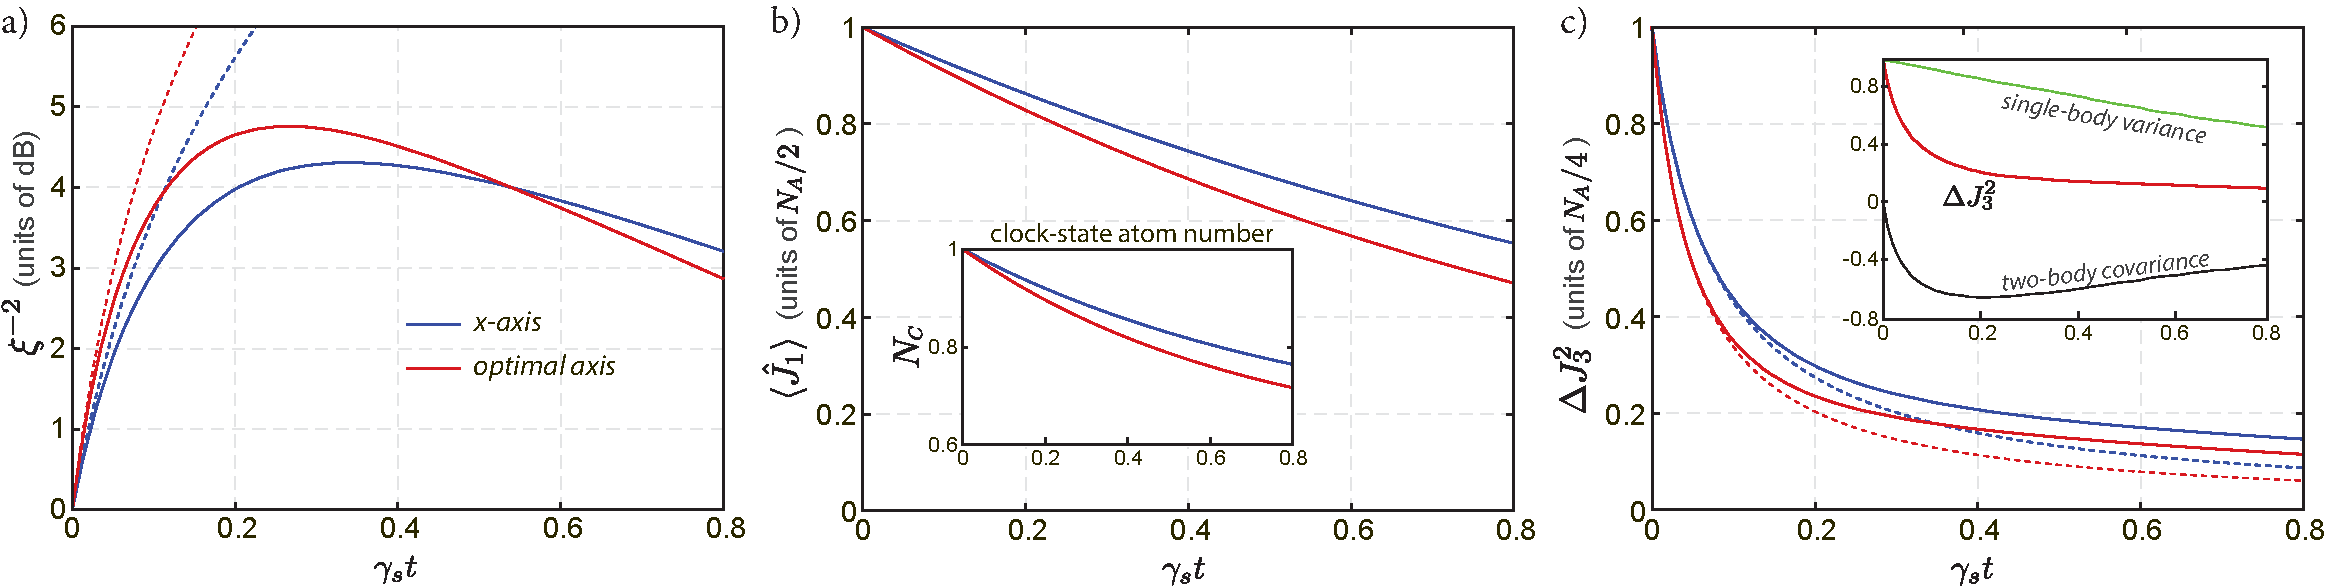
\includegraphics[scale=0.42]{../chap4/Fig4}
\caption[Squeezing on the clock states as a function of time in units of the scattering rate $\gamma_s$ for $2500$ atoms trapped in the $x$-$z$ plane at a distance $ r'\!_\perp=1.8a$ from the axis of the nanofiber.]{Squeezing on the clock states as a function of time in units of the scattering rate $\gamma_s$ for $2500$ atoms trapped in the $x$-$z$ plane at a distance $ r'\!_\perp=1.8a$ from the axis of the nanofiber. The optimal quantization axis (red) is compared to the quantization along the $x$ axis (blue). 
Dashed lines indicate simulations without optical pumping; i.e. no decoherence. 
(a) Metrological spin squeezing parameter $\xi^{-2}$, \erf{Eq::SqueezingParameter}, in dB. 
(b) Collective mean spin $\expt{\hat{J}_1}\equiv \expt{\hat{J}_x}$ and decaying atom number in the clock states, $N_C$ (inset).
(c) Conditional squeezed variance $\varz$. 
The inset shows the decomposition at the optimal quantization axis of $ \Delta J_3^2\equiv \Delta J_z^2 $ (red dashed) into the single-body variance, $N_A (\Delta j_z^{(1)})^2$ (green) and the two-body covariance, $N_A(N_A-1)\expect{\Delta j_z^{(1)}\Delta j_z^{(2)}}$ (black), as given by \erf{Eq::VarianceDecomposition}.
}\label{Fig::Squeezing_Dynamics}
\end{figure*}
%================


The peak squeezing is ultimately limited by the combined effects of optical pumping on both $\expt{\jx}$ and $\varz$.  Here, as in a free-space model \cite{baragiola_three-dimensional_2014}, the primary factor that limits metrological squeezing is the decay of the collective mean spin $\expt{\jx}$. 
A scattered photon eliminates the initial coherence between $\ket{\uparrow}$ and $\ket{\downarrow}$ within a single atom, thus depolarizing $\expt{\jx}$.  
Atoms optically pumped to magnetic sublevels outside of the clock subspace decay $N_C$, further reducing $\expt{\jx}$. 
These effects are captured by the depolarization rate $\gamma_{11}$ in the equation for $\expt{\jx}$, \erf{Eq::MeanSpinDecay}, whose solution is plotted in \frf{Fig::Squeezing_Dynamics}(b).
  
We can gain deeper understanding in the microscopic effects of optical pumping on spin squeezing by looking at the evolution of the one and two-body correlation functions.  In terms of its constituent pseudospins, the collective variance takes the form
	\begin{align} \label{Eq::VarianceDecomposition}
	\varz & = N_A \big( \Delta j_z^{(1)} \big)^2 + N_A(N_A-1) \expt{ \Delta j_z^{(1)} \Delta j_z^{(2)} }
	\end{align}
for permutationally symmetric states considered here, where $(1)$ and $(2)$ label any two atoms in the ensemble. Loss of atoms affects the first (single-body) variance term, which scales as $N_A$.
The two-body correlations which contribute as $N_A^2$ to the collective fluctuations, 
	\begin{align}
		\expt{ \Delta j_z^{(1)} \Delta j_z^{(2)} } &\equiv \smallfrac{1}{4} \big( \expt{ \hat{\sigma}_z^{(1)} \otimes \hat{\sigma}_z^{(2)}  } - \expt{\hat{\sigma}_z^{(1)} }^2  \big).
\end{align}
have a much larger influence on the total variance. Spin-spin correlations at the heart of spin squeezing, $\expt{ \hat{\sigma}_z^{(1)} \otimes \hat{\sigma}_z^{(2)} }$, rapidly generated by the measurement backaction decohere by optical pumping according to Eqs. (\ref{Eq::TwoBodyDecay}--\ref{Eq::OperatorMap}),
	\begin{align} \label{Eq::TwoBodySpinDecay}
		\frac{d}{dt} \expt{\hat{\sigma}_z^{(1)} \otimes \hat{\sigma}_z^{(2)} }  \Big|_{\rm op} = - 2 \gamma_{33}  \expt{\hat{\sigma}_z^{(1)} \otimes \hat{\sigma}_z^{(2)}} + \gamma_{30} \expt{ \hat{\mathbbm{1}}^{(1)}_C \otimes \hat{\sigma}_z^{(2)} + \hat{\sigma}_z^{(1)} \otimes \hat{\mathbbm{1}}^{(2)}_C },
	\end{align}
where $\hat{\mathbbm{1}}^{(n)}_C \equiv \big( \op{\uparrow}{\uparrow} + \op{\downarrow}{\downarrow} \big){}^{(n)}$ is the single-body projector onto the clock states.   
In addition, atoms that return to the clock subspace after scattering a photon inject additional noise into $\varz$.  
All of these effects are included in the equation for $\varz$, \erf{Eq::varJz}, whose overall and decomposed dynamical evolutions are shown in Fig. \ref{Fig::Squeezing_Dynamics}(c). 


%========= FIGURE: Peak squeezing (\xi, measurement strength, scattering rates) =========
\begin{figure}[!htbp]
\centering
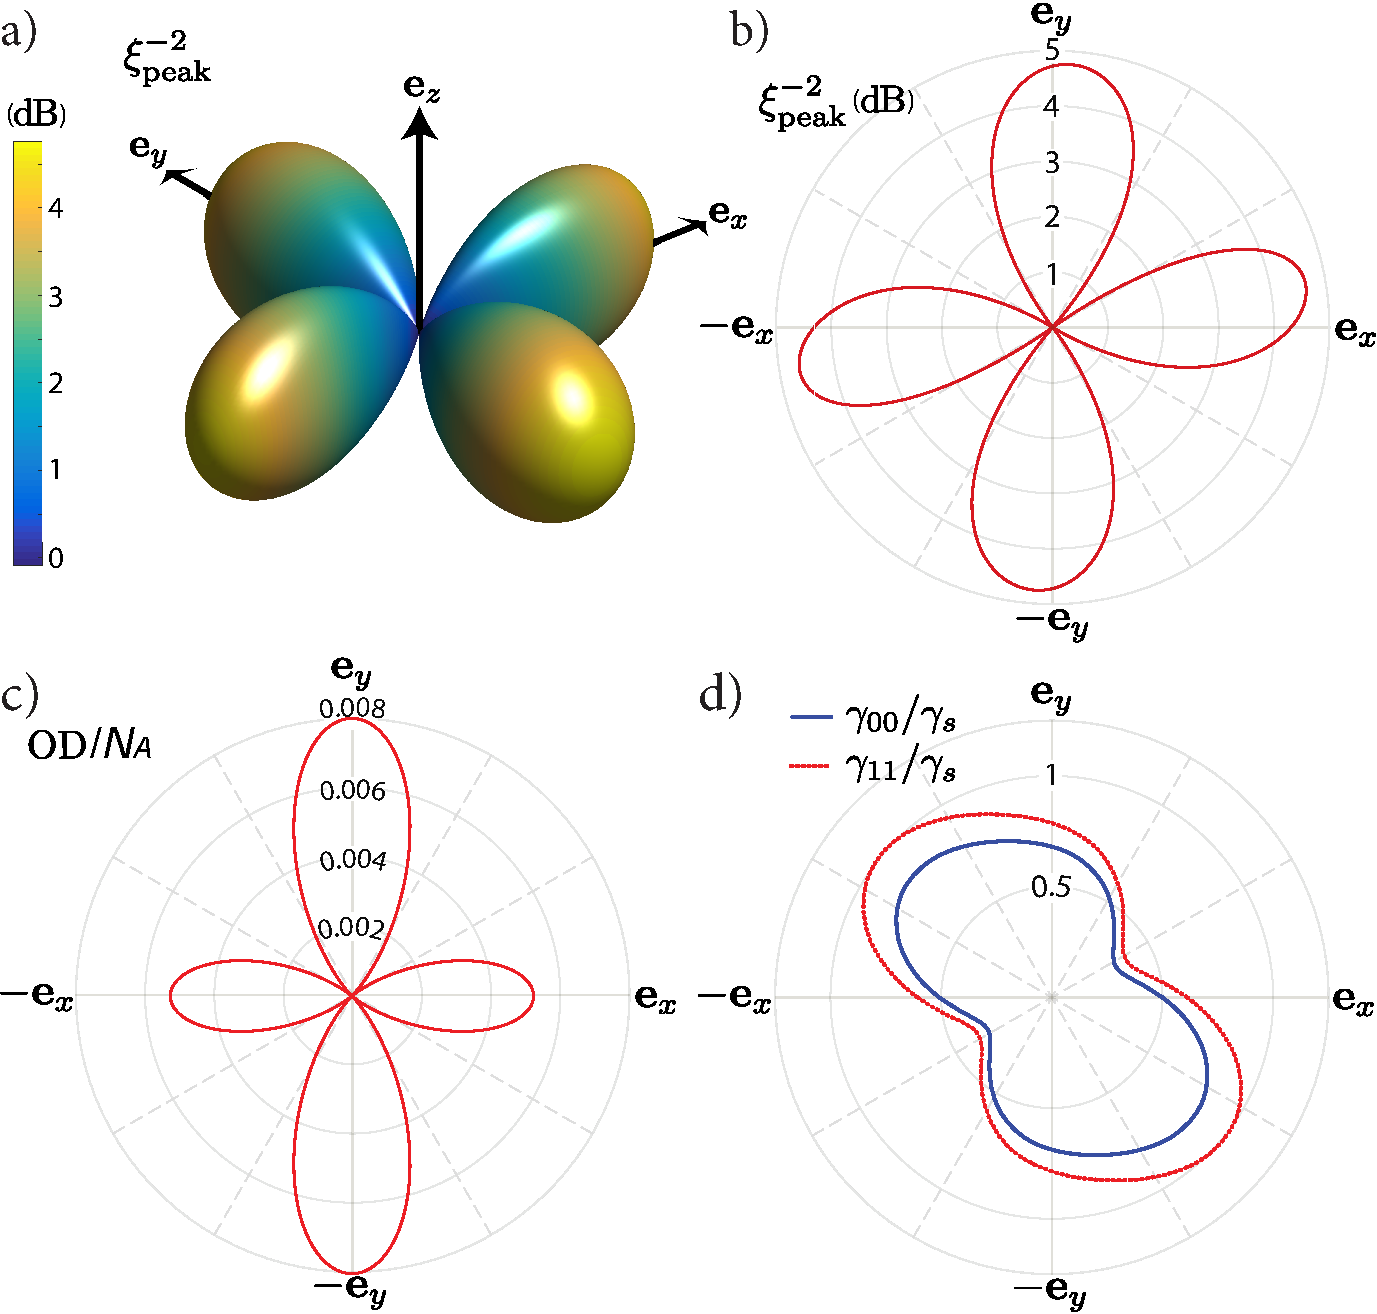
\includegraphics[scale=0.5]{../chap4/Fig5}
\caption[Dependence of the parameters that determine metrological squeezing  on the direction of the quantization axis that defines the clock states, $\mathbf{e}_{\tilde{z}}$.]{Dependence of the parameters that determine metrological squeezing  on the direction of the quantization axis that defines the clock states, $\qaxis$.  In all cases we consider $2500$ atoms trapped in the $x$-$z$ plane at distance $ r'\!_\perp=1.8a$ from the axis of the nanofiber. 
In (b--d) $\qaxis$ is confined to the $x$-$y$ plane, where the optimal peak squeezing occurs.
(a,b)  Peak achievable squeezing at the maximum time, measured in dB, as a function of the direction of  $\qaxis$. 
(c) OD/$N_A$=$\sigma_0 A_{in}/A^2_{J_z}$, \erf{Eq::OD/atom}.
(d) Rates of atom loss, $\gamma_{00}$, and depolarization, $\gamma_{11}$ relative to the characteristic scattering rate $\gamma_s$.  See Eqs.~\eqref{Eq::lrate} and~\eqref{Eq::frate}. }\label{Fig::Squeezing_QuantizationAxis}
\end{figure}
%================


With our model, we explore optimal conditions for generating spin squeezing.   The choice of quantization axis $\qaxis$ that defines clock states affects both the measurement strength and the relative rates of optical pumping. We plot the peak squeezing as a function of the direction of $\qaxis$ in the $x$-$y$ plane in \frf{Fig::Squeezing_QuantizationAxis}(b). 
We gain insight into the tradeoffs between QND entangling interaction and decoherence by independent inspection of the measurement strength and optical pumping rates.  
First, the rate of squeezing is determined by the effective optical density per atom on resonance,
\begin{align}\label{Eq::OD/atom}
\mathrm{OD}/N_A \equiv \frac{\kappa}{\gamma_s}=\frac{\sigma_0 A_{\rm in}}{A_{J_z}^2},
\end{align} 
which peaks when $\qaxis$ is along the $y$ axis, as seen in \frf{Fig::Squeezing_QuantizationAxis}(c). 
Choosing $\qaxis$ along $y$, the OD/$N_A$ is about 50\% larger than along $x$ axis.  
The various forms of decoherence similarly vary with quantization axis, as seen in \frf{Fig::Squeezing_QuantizationAxis}(d), where we plot the dominant rate of atom loss, $\gamma_{00}$, and the depolarization rate of the mean pseudospin $\expt{\jx}$, $\gamma_{11}$. 
Because the magic frequency $\magic{4}$ is nearly equidistant from $f'=3$ and $f'=4$ when the quantization  axis is near the $y$ axis (see \frf{Fig::CouplingStrength}(b)) this choice of quantization axis provides more protection from decoherence.   
While the decoherence rates in \frf{Fig::Squeezing_QuantizationAxis}(d) are largest near the $y$ axis, the increase in $\kappa$ more than compensates to provide optimal peak squeezing.

Finally, we explore the optimal conditions as a function of the trapping geometry.  
The dispersive entangling interaction is based on the collective atomic coupling to the evanescent guided-mode fields, which decay exponentially away from the nanofiber surface, as seen in OD/$N_A$ plotted in \frf{Fig::Squeezing_Distance}(a). 
From Eq.~\eqref{Eq::varJz}, the optimal choice of quantization axis depends not only on distance from the fiber but also weakly on the atom number, \frf{Fig::Squeezing_Distance}(b) because of the competition between squeezing and decoherence.  
At the optimal quantization axis, the strong dependence of peak achievable squeezing on distance from the fiber is as seen in \frf{Fig::Squeezing_Distance}(c) along with the expected increase as more atoms contribute to the atom-light interface.  

Several effects limit the reliability of the simulations for atoms trapped very near the fiber surface as $r'\!_\perp \rightarrow a$. 
First, strong van der Waals interactions modify the light shifts and magic frequencies \cite{vetsch_eugen_optical_2010, lacroute_state-insensitive_2012}.  
Second, the optical pumping model used here breaks down when the local density of states is significantly modified by the presence of the dielectric nanofiber \cite{LeKien2005a, le_kien_scattering_2006}. 
At distances $r'\!_\perp > 1.5a$ the atoms' local environment is roughly that of unmodified vacuum \cite{LeKien2005a} and a free-space optical pumping model in \erf{Eq::OpticalPumpingMapSchr} suffices. 


%======= FIG: Scaling with atom number and distance =======
\begin{figure*}[t]
\centering
\hspace{-50pt}
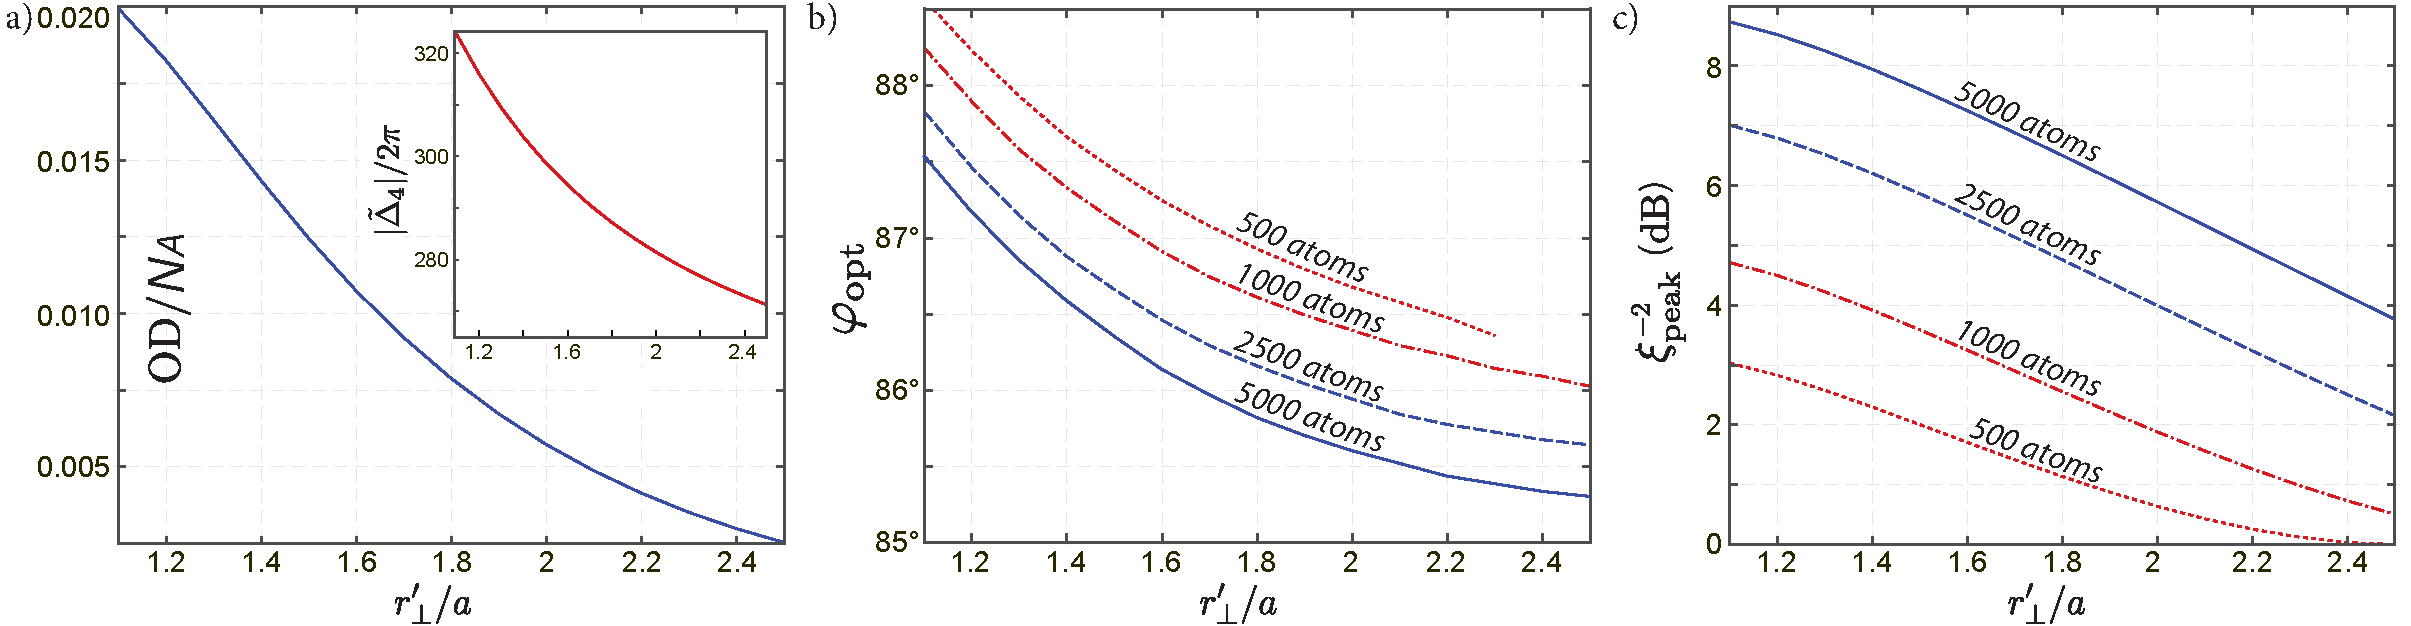
\includegraphics[scale=0.41]{../chap4/Fig6}
\caption[Parameters that define squeezing as a function of trapping distance $r'_\perp$ and initial atom number $N_A$.]{Parameters that define squeezing as a function of trapping distance $r'_\perp$ and initial atom number $N_A$. (a) OD/$N_A$. Inset is the corresponding magic detuning in units of MHz (see text).
(b) Optimal quantization axis orientation angle $\qaxis$ in the $x$-$y$ plane for different atom numbers. 
The line with $ 500 $ atoms terminates when the squeezing effect is too weak to be observed ($ r'\!_\perp>2.3a $).
(c) Peak metrological squeezing at the optimal $\qaxis$ for different atom numbers.} \label{Fig::Squeezing_Distance}
\end{figure*}
%================================


%====== SECTION: Summary and outlook ======%
\section{Summary and Outlook} \label{Sec::Conclusion}

We studied the strong cooperativity in the atom-light interface that can be achieved based on atoms trapped in the evanescent field surrounding an optical nanofiber, and interacting with a guided mode in the dispersive regime. 
The key parameter that determines the coupling is the resonant optical density per atom. 
Due to the tight confinement of the guided mode over the entire chain of atoms this parameter is $ \mathrm{OD}/N_A\sim 10^{-2} $ for typical geometries used in current experiments, which approaches that achieved for atomic ensembles trapped inside optical cavities of moderate finesse \cite{chen_conditional_2011, zhang_collective_2012}.  
In contrast, the atom-light coupling for atoms in free space is typically orders of magnitude smaller, $ \mathrm{OD}/N_A \sim 10^{-6}$.  
Under ideal conditions the atom-light interaction is entirely symmetric along the nanofiber, providing a platform for long-range correlations independent of distance between the atoms. 
As the light is entirely guided, fiber- or waveguide-coupled atomic ensembles can be networked together or coupled to other physical systems in a hybrid platform \cite{hafezi_atomic_2012, liebermeister_tapered_2014, Meng2015nanowaveguide, Tiecke2015Efficient} for truly long-range entanglement generation and distribution. 

We calculated the dispersive response based on a modal decomposition of the dyadic Green's function, which provides a general method to calculate the induced phase shifts and polarization rotations of the guided modes. 
With this we studied the QND measurement of atoms via polarization spectroscopy. 
In particular, we studied squeezing of the collective pseudospin associated the atomic clock states of cesium. 
The atoms induce a birefringent index of refraction on the light, conditional on the spin state, which provides a mechanism for measuring the atomic spin projection and thus squeezing its uncertainty.  
Based on our formalism we calculated the nanofiber-enhanced measurement strength that determines the rate of squeezing.  

The peak squeezing one can generate depends on a detailed balance between the reduction of spin projection noise based on QND measurement and the damage done to the spin ensemble due to optical pumping.  
Both measurement and optical pumping arise from the same physical mechanism -- scattering of photons by atoms.  
The former corresponds to cooperative forward scattering into the guided mode whereas the latter corresponds to local scattering into all other modes, primarily the unguided ``radiation" modes.   The cooperativity, specified by the effective OD/$N_A$, determines the ratio of these two effects and thus the ultimate power of the quantum atom-light interface. 

We studied QND measurement using a first-principles stochastic master equation model, which allowed us to track the atomic correlation functions that define the metrologically relevant squeezing parameter.  
These include the atomic projection noise uncertainty as well as the length of the collective spin vector that defines the metrological signal.  We find that decoherence acts primarily to depolarize the mean pseudospin and optically pump atoms out of the clock subspace, which we treat as loss.  In addition, optical pumping decoheres the spin correlations at the heart of spin squeezing, but at a reduced rate compared with the effect on the mean pseudospin.  
The combined effect of QND measurement and decoherence yields a peak squeezing approaching 5 dB with $\sim 2500$ atoms. Larger enhancements in atom-light coupling and QND squeezing are possible with modest increases in the number of trapped atoms and/or for atoms trapped closer to the nanofiber surface.  

Whereas we have assumed here that atoms can be prepared in a desired clock state defined by a particular quantization axis, in practice such preparation will require optical pumping that may be challenging for atoms near the surface of the nanofiber.   In addition, though we have treated the atoms as localized at well defined points, in practice the atoms' thermal motion can reduce the strong coupling described here.  Our formalism  provides a starting point for developing models necessary to study the dynamics of optical pumping, including the possibility of cooling atoms to the vibrational ground state, where thermal motion is negligible. 

Finally, though we have treated here the case of strong coupling due solely to tight confinement of the guided mode for atoms near the surface of the nanofiber,  we can achieve even greater enhancement  by combining this effect with longitudinal confinement provided by fiber-based optical cavities~\cite{le_kien_intracavity_2009, wuttke_nanofiber_2012, yalla_cavity_2014, bohnet_reduced_2014, nayak_optical_2014}.  
The coupling can be further improved under EIT conditions that substantially slow the group velocity \cite{gouraud_demonstration_2015, sayrin_storage_2015, kumar_autler-townes_2015, le_kien_electromagnetically_2015}.  In addition, quantum control of the internal hyperfine state \cite{smith_quantum_2013-1} can greatly enhance the entangling power of the atom-light interface~\cite{trail_strongly_2010, norris_enhanced_2012}. 
For large enough coupling, QND measurement should allow production of highly entangled spin states beyond the Gaussian regime \cite{stockton_deterministic_2004, mcconnell_entanglement_2015}.

%</birefringenceprotocol>

ACKNOWLEDGMENTS 
We gratefully acknowledge Sudhakar Prasad for helpful discussions regarding the dyadic Green's function. 
We thank the UNM Center for Advanced Research Computing for computational resources used in this work. 
This work was support by the AFOSR, under grant Y600242, and the NSF, under grants PHY-1212445, 1307520. 

\appendix

%=========== APPENDIX ===========%
%\chapter[Deriving birefringence QND measurement dynamics]{Some detailed derivation of the birefringence QND measurement dynamics}

%<*atomnumberdetection>
\chapter[Minimum detectable atom number in a measurement protocol]{Minimum detectable atom number using the birefringence effect of a nanofiber}\label{sec:birefringenceresolution}
The Faraday spectroscopy theory for optical lattice has been published in Ref.~\cite{Smith2003a}. Following this thread, we present the birefringence spectroscopy analysis for our nanofiber case.

\section[Shot-noise limit and minimum detectable atom number]{Shot-noise limit and minimum detectable \\ atom number}
To measure the Stocks vector rotation angle on the \Poincare sphere, that is the transformation of the polarization of the light, we launch a probe light along the bisection line between $ x $ and $ y $ axes, and trap the atom on the $ x $ axis, and then measure the output powers of the counterclockwise-rotating ($ \sigma_+ $) and the clockwise-rotating ($ \sigma_- $) components of the output. From Eq.~\eqref{eq:birefringencerotang} and considering the quantum transition factor factor in the Hamiltonian, Eq.~\eqref{Eq::RotationAngle}, the total differential phase shift between the $ \sigma_+ $ and $ \sigma_- $ components of the probed traveling light interacted with $ N_A $ atoms can be given by
\begin{align}
\varphi_{_N} &= N_A C_{j'}^{(0)}\sigma_0\frac{c}{v_g}\frac{\Gamma_0}{4\Delta}\left[| \mathbf{u}_H(r'_{\!\perp})|^2- | \mathbf{u}_V(r'_{\!\perp})|^2 \right],
\end{align}
where $ C_{j'}^{(0)}=C_{j'f}^{(0)}=\sum_{f,f'}C_{f,f'}^{(0)}=\frac{2^{j'-1/2}}{3} $ are the far-detuning rank-$ 0 $ coefficient on a $ j\rightarrow j' $ transition, which is $ \frac{1}{3} $ for the D1 line transition and $ 2/3 $ for the D2 line transition for the alkali atoms we study~\cite{Deutsch2010a}. 
The transformation of polarization is measured in terms of the total power difference between the $ x $- and $ y $-components of the field. The measured signal power is given by
\begin{align}
\Delta P_S &= P_0 \sin(\varphi_{_N}) \approx P_0 \varphi_{_N}, \label{eq:polsignal}
\end{align}
where $ P_0 $ is the power of the signal, and we have assumed the rotation angle is very small for our study case. 

Our resolution of detection is limited by the shot noise characterized by the fluctuations in the power difference with a root mean square amplitude of 
\begin{align}
\Delta P_{SN} &= \sqrt{\frac{P_0 \hbar \omega_0 }{2\eta \tau_{pd}}}, \label{eq:shotnoise}
\end{align}
where $ \eta $ is the quantum efficiency of the detector, and $ \tau_{pd} $ is the response time of the photon detector.
In the extreme case that the signal is equal to the shot noise, that is to make $ \Delta P_S=\Delta P_{SN} $, we can obtain the minimum number of atoms that we can detect (the resolution) as
\begin{align}
N_{min} &= \frac{1}{C_{j'}^{(0)}}\sqrt{\frac{8  \hbar \omega_0  }{P_0\eta \tau_{pd}}}\frac{\Delta}{\sigma_0 n_g\Gamma_0}\frac{1}{\left[| \mathbf{u}_H(r'_{\!\perp})|^2- | \mathbf{u}_V(r'_{\!\perp})|^2 \right]}\\
&=\frac{1}{C_{j'}^{(0)}} \sqrt{\frac{8  \hbar \omega_0  }{P_0\eta \tau_{pd}}}\frac{2\pi\Delta}{3\lambda^2 \frac{4}{3} \left( \frac{\omega_0}{c}\right)^3 \frac{|d_{eg}|^2}{\hbar}}\frac{A_{e\!f\!f}^V}{\zeta -1 }\\
&= \frac{1}{C_{j'}^{(0)}}\sqrt{\frac{\hbar^3 \pi c  }{P_0\eta \tau_{pd}\lambda}}\frac{\lambda\Delta }{  \left( 2\pi\right)^2 |d_{eg}|^2}\frac{A_{e\!f\!f}^V}{\zeta -1 }\\
&= \frac{1}{4\pi C_{j'}^{(0)}}\sqrt{\frac{\hbar^3 c \lambda }{\pi P_0\eta \tau_{pd}}}\frac{\Delta }{   |d_{eg}|^2}\frac{A_{e\!f\!f}^V}{\zeta -1 },\label{eq:Nmin_birefringence}
\end{align}
with
\begin{align}
A_{e\!f\!f}^V &= \frac{1}{n_g| \mathbf{u}_V(r'_{\!\perp})|^2}\\
\zeta &= \frac{| \mathbf{u}_H(r'_{\!\perp})|^2}{| \mathbf{u}_V(r'_{\!\perp})|^2}.
\end{align}
Eq.~\eqref{eq:Nmin_birefringence} is the formula to find the minimum detectable atom number in the shot-noise limit if all practical parameters are known for the experiment. Below, we estimate $ N_{min} $ when the detector is ideal for the measurement protocol.

\section{Estimate the minimum detectable atom number in an ideal case}
We consider the critical time scale that 
\begin{align}
\tau_{pd} &= \frac{1}{\gamma_s},
\end{align}
where $ \gamma_{s} $ is the photon scattering rate (see Appendix~\ref{chap:summaryofatomicphysicsformulas}). The minimum detectable atom number can be estimated using the relationship between the scattering rate and the scattering cross section $ \sigma(\Delta) $ or the saturation cross section $ \sigma_0 $ under the critical time scale. Now that
\begin{align}
\gamma_s &= \sigma(\Delta) \frac{I(\br')}{\hbar \omega_0} \\
\sigma(\Delta) &=\frac{\sigma_0}{1+\frac{4\Delta^2}{\Gamma^2_0}}\approx \sigma_0 \frac{\Gamma_0^2}{4\Delta^2} \quad \text{(far detuning)}
\end{align}
where $ I(\br') $ is the light intensity at the atom position.
Hence,
\begin{align}
\gamma_s &\approx \sigma_0\frac{\Gamma_0^2}{4\Delta^2} \frac{I(\br')}{\hbar \omega_0}=\frac{\sigma_0}{A_{in}}\frac{P_0}{\hbar\omega_0}\frac{\Gamma_0^2}{4\Delta^2},
\end{align}
where the effective incident mode area at the atom position, $A_{in}  $, is defined as
\begin{align}
A_{in }&= \frac{P_0}{I(\br')}.
\end{align}

We also set the quantum efficiency $ \eta=1 $. The critical shot noise defined in Eq.~\eqref{eq:shotnoise} then becomes
\begin{align}
\Delta P_{SN} &\approx \sqrt{\frac{P_0 \hbar \omega_0 \gamma_s}{2\eta }} =P_0\sqrt{\frac{ \sigma_0 }{2A_{in}}}\frac{\Gamma_0}{2\Delta}.
\end{align}
The signal defined in Eq.~\eqref{eq:polsignal} can be rewritten as
\begin{align}
\Delta P_S &= {N_A P_0}{C_{j'}^{(0)}} \frac{\sigma_0}{\Abir}\frac{\Gamma_0}{4\Delta},
\end{align}
where the effective mode area at the atom position for our configuration is defined by
\begin{align}
\Abir &= \frac{1}{n_g}\frac{1}{| \mathbf{u}_H(r'_{\!\perp})|^2- | \mathbf{u}_V(r'_{\!\perp})|^2}.
\end{align}
If we make the shot noise power equal to the minimum detectable signal power, we can obtain the minimum detectable atom number as
\begin{align}
N_{min} &= \frac{1}{C_{j'}^{(0)}}\sqrt{\frac{2\Abir^2}{A_{in}\sigma_0}}.
\end{align}
As an estimate of the scale, we can ignore the constant factor of $ \sqrt{2} $ and claim the minimum detectable atom number is on the order of 
\begin{align}
\delta N_A \sim \frac{1}{C_{j'}^{(0)}}\sqrt{\frac{\Abir^2}{A_{in}\sigma_0}}=\frac{1}{C_{j'}^{(0)}}\sqrt{\frac{\mathrm{OD}}{N_A}},
\end{align}
where $ \mathrm{OD}/N_A=\frac{\Abir^2}{A_{in}\sigma_0} $ is the optical depth per atom for this birefringence measurement configuration using mixed states of atoms. 

%</atomnumberdetection>

%=========== APPENDIX: Nanofiber mode functions ===========%
\chapter{Guided-mode functions for the optical nanofiber} \label{chap:fibereigenmodes}

  

In this Appendix we provide, for reference, the fundamental HE$_{11}$ solutions to the homogeneous wave equation, \erf{Eq::WaveEquationSource} with $\tensor{\boldsymbol{\alpha}} = 0$, for a cylindrical nanofiber of radius $a$ and index of refraction given by \erf{Eq::IndexofRefraction}.  At a given frequency, $\omega_0 = c k_0$, the magnitudes of the longitudinal and transverse wave vectors for a guided mode are related by $n^2 k_0^2 = \beta_0^2 + k_\perp^2$.  
The positive propagation constant, $\beta_0 \equiv \beta(\omega_0)$, is determined from the eigenvalue equation that results from enforcing physical boundary conditions at the fiber surface \cite{Snyder1983Optical},
	\begin{align}
		\frac{J_0(ha)}{ha J_x(ha)} = - \frac{n_1^2+n_2^2}{2n_1^2} \frac{K'(qa)}{qa K_1(qa)} + \frac{1}{h^2 a^2} - \bigg[ \bigg(\frac{n_1^2 - n_2^2}{2 n_1^2} \frac{K'(qa)}{qa K_1(qa)} \bigg)^2  + \frac{\beta_0^2}{n^2_1 k^2} \bigg(\frac{1}{q^2a^2} + \frac{1}{h^2a^2} \bigg)^2 \bigg]^{1/2}.
	\end{align}
Inside the nanofiber the transverse wavevector is real, $k_\perp = q$, where $q=\sqrt{\beta_0^2- n_2^2k_0^2}$, and outside the nanofiber it is purely imaginary, $k_\perp = i h$, where $h=\sqrt{n_1^2 k_0^2 - \beta_0^2}$.  The vector eigenfunctions are expressed as $\mbf{f}_{\mu}(\br) = (2\pi)^{-1/2}\mbf{u}_{b,p}(\mbf{r}_\perp) e^{i b \beta_0 z}$, where the modes are indexed by frequency $\omega_0$, propagation direction $b = \pm$, and polarization $p$.

A relatively simple form for the guided-mode functions can be expressed in a cylindrical basis $(r_\perp, \phi, z)$ with longitudinal unit vector $\mathbf{e}_z$, oriented along the fiber axis.  
The transverse unit vectors are related to their fixed Cartesian counterparts via the relations
\begin{subequations}
	\begin{align}
		\mathbf{e}_{r_{\!\perp}}     &= \mathbf{e}_x \cos \phi + \mathbf{e}_y \sin \phi, \\
		\mathbf{e}_\phi &= - \mathbf{e}_x \sin \phi + \mathbf{e}_y \cos \phi.
	\end{align}
\end{subequations}
The transverse profile for the quasicircular guided modes, $p = \pm$, is
	\begin{align} \label{Eq::QuasicircularModes}
		\mbf{u}_{b,\pm}(\mathbf{r}_\perp) = \big[\mathbf{e}_{r_{\!\perp}} u_{r_{\!\perp}}(r_\perp) \pm i \mathbf{e}_\phi u_\phi(r_\perp) +  i b \mathbf{e}_z  u_z(r_\perp) \big]e^{ \pm i \phi}, 
	\end{align}
and for the quasilinear guided modes, $p = \{H,V\}$, is
	\begin{subequations} \label{Eq::QuasilinearModes}
	\begin{align}
		\mbf{u}_{b,H}(\mathbf{r}_\perp) = & \sqrt{2} \big[ \mathbf{e}_{r_{\!\perp}} u_{r_{\!\perp}}(r_\perp) \cos \phi - \mathbf{e}_\phi u_\phi(r_\perp) \sin \phi +  ib \mathbf{e}_z  u_z(r_\perp) \cos \phi \big] \\
		\mbf{u}_{b,V}(\mathbf{r}_\perp) = & \sqrt{2} \big[ \mathbf{e}_{r_{\!\perp}} u_{r_{\!\perp}}(r_\perp) \sin \phi + \mathbf{e}_\phi u_\phi(r_\perp) \cos \phi +  ib \mathbf{e}_z  u_z(r_\perp) \sin \phi \big]. 
	\end{align}
	\end{subequations}
The modes are expressed in terms of real-valued functions that depend only on the radial coordinate $r_\perp$,
	\begin{subequations} \label{Eq::ProfileFunctions}
	\begin{align} 
		u_{r_{\!\perp}}(r_\perp) =& u_0 \big[ (1-s) K_0(q{r_{\!\perp}}) + (1+s)K_2(q{r_{\!\perp}})\big] \\
		u_\phi(r_\perp) =& u_0\big[ (1-s) K_0(q{r_{\!\perp}}) - (1+s)K_2(q{r_{\!\perp}})\big] \\
		u_z(r_\perp) =& u_0 \frac{2 q}{\beta_0} \frac{K_1(qa)}{J_x(ha)} J_x(h{r_{\!\perp}}), \label{Eq::zprofile}
	\end{align}
	\end{subequations}
where $u_0$ is set by the normalization condition, $\int d^2 \mathbf{r}_\perp n(r_\perp) | \mathbf{u}_\mu(\br_\perp)|^2=1$, $J_n$ and $K_n$ are the $n^{th}$ Bessel functions of the first and second kind, $f'(x)$ indicates a derivative with respect to the argument $x$, and 
	\begin{align}
		s = \frac{1/(q^2 a^2)^{2} + 1/(h^2 a^2)^{2}}{[J'_1(ha)/haJ_x(ha) + K'_1(qa)/qaK_1(qa)]}.
	\end{align}  
Of particular interest is the $z$-component, \erf{Eq::zprofile}, which can become appreciable.  Note that the phase convention in Eqs. (\ref{Eq::QuasicircularModes}-\ref{Eq::ProfileFunctions}) has been chosen to emphasize properties of the quasilinear modes and differs from that of \emph{Le Kien et al.} -- for instance in Ref. \cite{le_kien_propagation_2014}.  
Further details about the guided-mode fields inside the nanofiber ($r_\perp\leq a$), the radiation (unguided) modes, and the quantized form of both can be found in Refs. \cite{Sondergaard2001, tong_single-mode_2004, Kien2004, LeKien2005a, vetsch_eugen_optical_2010}.



%<*birefringencerates>
%===================APPENDIX: Photon scattering and optical pumping rates =====================%
\chapter{Photon scattering and optical pumping rates} \label{Appendix::Rates}	

In this Appendix we give the explicit expressions for the photon scattering rates used in Sec.~\ref{Sec::QNDMeasurement} following the formalism given in~\cite{deutsch_quantum_2010}.  The total rate of photon scattering by an atom in the clock state $\ket{f,0}$ is
	\begin{equation}\label{Eq::gammaf}
		\gamma_{f}=- \frac{2}{\hbar} {\rm Im} \big[ \bra{f,0} \hat{h}_{\rm eff}\ket{f,0} \big] ,
	\end{equation}
where the effective non-Hermitian light-shift Hamiltonian for one atom is 
\begin{align}
\hat{h}_{\rm eff} = - \hat{\mathbf{E}}^{(-)}_{\rm in}(\mathbf{r}' ; t ) \cdot \poltens \cdot \hat{\mathbf{E}}^{(+)}_{\rm in}(\mathbf{r}' ;t )
\end{align}
as follows from \erf{Eq::LightShiftHam}, where $\charpol = -\frac{\sigma_0}{8\pi k_0}\frac{\Gamma}{\Delta_{ff'}+i\Gamma/2}$ is the complex polarizability and the irreducible tensor operator $ \hat{\tensor{\mbf{A}}}(f,f') $ is given in \erf{Eq::PolarizabilityIrrep}.


The rate of optical pumping between clock states $\ket{f,0} \rightarrow \ket{\tilde{f},0}$ is
	\begin{equation}\label{Eq::gammaff}
		\gamma_{f \rightarrow \tilde{f} } 
		=\sum_{q}\big| \bra{\tilde{f},0} \hat{W}_q^{\tilde{f}f} \ket{f,0} \big|^2,
	\end{equation}
where $ \hat{W}_q^{\tilde{f}f} = \sum_{f'}\frac{\Omega/2}{\Delta_{f'\tilde{f}}+i\Gamma/2}(\mathbf{e}_q^*\cdot\hat{\mathbf{D}}_{\tilde{f} f'} )(\mathbf{e}_{\rm in}\cdot \hat{\mathbf{D}}^\dagger_{f'f} ) $ are the Lindblad jump operators for optical pumping between ground levels $ f\rightarrow \tilde{f} $~\cite{deutsch_quantum_2010}. 
Each jump operator $\hat{W}_q^{\tilde{f}f}$ is associated with absorption of the probe photon polarized along $ \mathbf{e}_{\rm in} $ followed by spontaneous emission of a photon with polarization $ \mathbf{e}_q $, where $q= \{0,\pm 1\}$ labels spherical basis elements for $\pi$ and $ \sigma_\pm$ transitions.  

To find the dependence on the input field intensity, we define a characteristic photon scattering rate, $\gamma_s \equiv \frac{\Gamma\Omega^2}{4\Delta_{J_z}^2}= \frac{\sigma_0}{A_{\rm in}}\frac{\Gamma^2}{4 \Delta_{J_z}^2} \dot{N}_L $, with Rabi frequency $ \Omega=2\bra{j}|d|\ket{j'}\mathcal{E}^{(+)}_{\rm in}/\hbar $, reduced optical dipole matrix element $\bra{j}|d|\ket{j'}$, and field amplitude $ \mathcal{E}^{(+)}_{\rm in}=|\mathbf{E}_{\rm in}^{(+)}(\br')| $.
Eqs.~\eqref{Eq::gammaf} and~\eqref{Eq::gammaff} yield,
\begin{subequations}
	\begin{align}
		\gamma_f &=n_g\dot{N}_L  \sum_{f'} \sigma (\Delta_{ff'} ) \mathbf{u}^*_\inp(\br'_\perp)\cdot \bra{f,0} \hat{\tensor{\mbf{A}}}(f,f') \ket{f,0}  \cdot \mathbf{u}_\inp(\br'_\perp)\\
		&= \dot{N}_L\frac{\pi \omega_0}{\hbar v_g} \!\!\sum_{f'\! , q}\! \frac{\Gamma |\bra{j'}|d|\ket{j}|^2}{\Delta_{ff'}^2+\Gamma^2/4} |o^{j'f'}_{jf}\! C^{f 0;1q}_{f' q}|^2  
		|\mathbf{e}_q \!\cdot\! 
		\left( \mathbf{u}_{H}^*(\br^\prime\!\!_\perp) \!+\! 
		\mathbf{u}_{V}^*(\br^\prime\!\!_\perp)\right) |^2\\
		&\approx  \gamma_s \sum_{f'} \frac{\Delta_{J_z}^2}{\Delta_{ff'}^2}\sum_q \big| o_{jf}^{j'f'}C_{f'q}^{f0;1 q} \big|^2 \mathbf{e}_q^* \cdot (\mathbf{e}_{\rm in}\mathbf{e}_{\rm in}^* )\cdot \mathbf{e}_q, 
	\end{align}
\end{subequations}
\begin{subequations}
	\begin{align}
		\gamma_{f \rightarrow \tilde{f}} &= \frac{\Gamma\Omega^2(\mathbf{r}')}{4}\sum_{f',q}   \frac{ \left|o^{j'f'}_{j\tilde{f}}\! o^{j'f'}_{jf}\!  C^{\tilde{f} 0;1q}_{f' q}\! C^{f 0;1q}_{f' q}\! \left(\mathbf{e}^*_{q}\! \cdot\! \mathbf{e}_{\rm in} \right)\right|^2}{ \Delta_{ff'}^2 \!\!+\! \Gamma^2/4}\\
		&\approx \gamma_s \sum_{f'} \frac{\Delta_{J_z}^2}{\Delta_{ff'}^2}\sum_q \big| o_{j\tilde{f}}^{j'f'} o_{jf}^{j'f'}C_{f'q}^{\tilde{f}0;1 q}C_{f'q}^{f0;1q} \big|^2 \mathbf{e}_q^* \cdot (\mathbf{e}_{\rm in}\mathbf{e}_{\rm in}^* )\cdot \mathbf{e}_q,
	\end{align}
\end{subequations}
where $ \sigma (\Delta_{ff'} )  = \sigma_0 \Gamma^2/4\Delta^2_{f' f}$ is the the scattering cross section at the probe detuning, $ C_{f'q}^{f0;1 q}=\Braket{f'q}{f0;1q}$ are the Clebsch-Gordan coefficients, and
\begin{equation}
\big| o_{jf}^{j'f'} \big|^2=(2j'+1)(2f+2) \bigg\{
\begin{array}{ccc}
f' & 7/2 & j' \\
 j & 1 & f 
 \end{array}
 \bigg\}
\end{equation}
are the relative oscillator strengths determined by the relevant Wigner 6-$J$ symbol. 
We have also expanded the jump operators as
\begin{align} \label{Eq::JumpOperators}
\hat{W}_q^{\tilde{f}f} 
&= \sum_{f'} \sqrt{\Gamma}\frac{\Omega(\mathbf{r}')/2}{ \Delta_{f'f} + i\Gamma/2} o^{j'f'}_{j\tilde{f}} o^{j'f'}_{jf}\nonumber\\
& \sum_{\tilde{m}=0,m=0,m'=q}\!\!\!\!\!\!\!\!\!\! C^{\tilde{f} \tilde{m};1q}_{f' m'} \sum_{q'=q}C^{f m;1q'}_{f' m'} \left(\mathbf{e}^*_{q'} \cdot\mathbf{e}_{\rm in} \right) \op{\tilde{f},\tilde{m}}{f,m}\nn\\
&= \sum_{f'} \!\!\frac{\sqrt{\Gamma}\Omega(\mathbf{r}')/2}{ \Delta_{f'f} \!\!+\! i\Gamma/2} o^{j'f'}_{j\tilde{f}}\! o^{j'f'}_{jf}\!  C^{\tilde{f} 0;1q}_{f' q}\! C^{f 0;1q}_{f' q}\! \left(\mathbf{e}^*_{q}\! \cdot\! \mathbf{e}_{\rm in} \right)\! \op{\tilde{f},0}{f,0}.
\end{align}
As shorthands, we also denote $ \gamma_{\tilde{f}f}=\gamma_{\tilde{f}\rightarrow f} $.

%</birefringencerates>

%<*birefringencemotioneq>
%===================APPENDIX: Equations of motion =====================%
\chapter[Equations of motion for the moments]{Derivation of the equations of motion for the moments} \label{Appendix::OpticalPumping}	

In this Appendix we derive the equations of motion for the correlation functions that define the metrologically relevant squeezing parameter, $\xi^2 = N_A \Delta J_z^2/\expt{\hat{J}_x}^2$.  
We seek the time evolution of the one and two-body correlation functions:
\begin{subequations}
\begin{align}
&\expt{\hat{N}_C} = \sum_n \expt{\hat{\mathbbm{1}}^{(n)}_C} \\
&\expt{\hat{J}_x} = \frac{1}{2} \sum_n \expt{\hat{\sigma}_x^{(n)}} \\
&\expt{\hat{J}_z} = \frac{1}{2} \sum_n \expt{\hat{\sigma}_z^{(n)}} \\
&\expt{\hat{J}_z^2} = \frac{\expt{\hat{N}_C}}{4} +\frac{1}{4} \sum_{m \neq n} \expt{\hat{\sigma}_z^{(m)}\otimes \hat{\sigma}_z^{(n)}}, 
\end{align}
\end{subequations}
where $\hat{\mathbbm{1}}_C \equiv \op{\uparrow}{\uparrow} + \op{\downarrow}{\downarrow}$ is the single-atom projector onto the clock states. 
To include optical pumping, we apply the following equations of motion. For a collective, single-body operator, $\hat{X} = \sum_n \hat{x}^{(n)}$, the evolution due to optical pumping is $d\expt{ \hat{X}}|_{\rm op} = \sum_n \Tr [\mathcal{D}_n[\hat{\rho}]\hat{X} ]dt = \sum_n \expt{\mathcal{D}_n\dg[\hat{x}^{(n)}]} dt$, where the map, which acts locally on atoms along the nanofiber, is given in \erf{Eq::OpticalPumpingMapSchr}.  
Two-body microscopic operators decay by optical pumping according to \cite{baragiola_three-dimensional_2014}
	\begin{align} \label{Eq::TwoBodyDecay}
		\frac{d}{dt} \expt{ \hat{x}^{(m)} \otimes \hat{y}^{(n)} } \Big|_{\rm op}= &\expt{ \mathcal{D}_m\dg[ \hat{x}^{(m)}] \otimes \hat{y}^{(n)} } + \expt{ \hat{x}^{(m)}\otimes \mathcal{D}_n\dg[ \hat{y}^{(n)}] },
	\end{align}
where the superscripts refer to the $m^{th}$ and $n^{th}$ atoms. 

\section{Summary of results}
Since the derivation is rather long, we first summarize the main results below, and then provide more details in the next section.

Applying the adjoint map to the single-atom operators yields 
	\begin{subequations} \label{Eq::OperatorMap}
	\begin{align}
		\mathcal{D}\dg[\hat{\mathbbm{1}}_C] & = - \gamma_{00} \hat{\mathbbm{1}}_C +\gamma_{03} \hat{\sigma}_z \label {Eq::Idecay} \\
		\mathcal{D}\dg[\hat{\sigma}_z] & =- \gamma_{33} \hat{\sigma}_z +  \gamma_{30} \hat{\mathbbm{1}}_C 
\label{Eq::zdecay} \\
		\mathcal{D}\dg[\hat{\sigma}_x] & = - \gamma_{11} \hat{\sigma}_x\label{Eq::xdecay},
	\end{align}
	\end{subequations}
with rates	
	\begin{subequations} \label{Eq::DecayRates}
	\begin{align}
		\gamma_{00} 
			& = \frac{\gamma_{\uparrow}+\gamma_{\downarrow} - \gammauu-\gammaud  -\gammadd-\gammadu}{2} \label{Eq::lrate} \\
			\gamma_{03} 
			& = \frac{-\gamma_{\uparrow}+\gamma_{\downarrow} +\gammauu + \gammaud - \gammadd - \gammadu }{2}\\		
		\gamma_{33} 
			& = \frac{\gamma_{\uparrow}+\gamma_{\downarrow} - \gammauu+\gammaud  -\gammadd+\gammadu}{2}\\
			\gamma_{30} 
			& = \frac{-\gamma_{\uparrow} + \gamma_{\downarrow} + \gammauu - \gammaud - \gammadd + \gammadu }{2} \\
			\gamma_{11} 
			& = \frac{\gamma_{\uparrow}+\gamma_{\downarrow}}{2}. \label{Eq::frate}
	\end{align}
	\end{subequations}
Given Eqs. (\ref{Eq::TwoBodyDecay}, \ref{Eq::OperatorMap}), the equations for the two-body spin correlations, \erf{Eq::TwoBodySpinDecay}, follow.  Similarly, one can derive equations of motion for the remaining two-body microscopic operator correlations $ \expt{\hat{\mathbbm{1}}^{(m)}_C \otimes \hat{\mathbbm{1}}^{(n)}_C} $ and $ \expt{\hat{\mathbbm{1}}^{(m)}_C \otimes \hat{\sigma}_z^{(n)} + \hat{\sigma}_z^{(m)} \otimes \hat{\mathbbm{1}}^{(n)}_C } $ when $ m\neq n $ and from these, the macroscopic operator expectation values $ \expt{\hat{J}_z^2} $, $ \expt{\hat{N}_C^2} $, and $ \expt{\hat{N}_C\hat{J}_z} $.  As we have examined numerically, on the time scale of the QND measurement, the correlation between atom number in the clock state subspace and the pseudospin moment is weak, and one can thus treat the atom number operator in the clock state subspace as a $c$-number.
We therefore set $ \expt{\hat{N}_C\hat{J}_z}-\expt{\hat{N}_C}\expt{\hat{J}_z} = 0 $ and $ \expt{\hat{N}_C^2} - \expt{\hat{N}_C}^2 = 0 $ and define $ N_C\equiv \expt{\hat{N}_C}$. 

The equations of motion for the moments of $\jz$ are now found from the SME, \erf{Eq::SME},
	\begin{subequations} \label{Eq::J3MomentEquations}
	\begin{align} 
		d \expt{\jz} =& s \sqrt{\kappa} \varz \, dW - \gamma_{33} \expt{\jz}dt + \smallfrac{1}{2} \gamma_{30} N_C dt ,  \\
		d \expt{\jz^2} =& 2 s\sqrt{\kappa} \expt{\jz}\Delta J_z^2 \, dW - 2 \gamma_{33} \expt{\jz^2}dt + \smallfrac{1}{4} \big( 2 \gamma_{33}-\gamma_{00}\big) N_C dt \\
		&+ \gamma_{30} \expt{\jz} N_C dt + \smallfrac{1}{2}\left(\gamma_{03} -2 \gamma_{30}\right) \expt{\jz} dt. \nonumber 
	\end{align}
	\end{subequations}
The stochastic term in $d\expt{\jz^2}$ was simplified by assuming Gaussian statistics \cite{jacobs_straightforward_2006}, $\expt{\jz^3} = 3\expt{\jz^2}\expt{\jz}- 2\expt{\jz}^3$. 
Finally, the It\={o} calculus governing the stochastically evolving moments requires that differentials be taken to second order, and the evolution of the variance is given by $d \varz = d \expt{\jz^2} - 2 \expt{\jz} d \expt{\jz} - ( d \expt{\jz} )^2$. 
The equation of motion for the conditional variance, \erf{Eq::varJz}, then follows from Eqs. \eqref{Eq::J3MomentEquations}.

\section{More details of the derivation}

In the \emph{clock-state}\index{state!clock state} case, we define $ \ket{\uparrow} = \ket{f=4,m=0} $, $ \ket{\downarrow}=\ket{f_3,m=0} $ for an arbitrary $ i $-th atom. 
There are some useful properties we can use for our calculations below:
\begin{align}
\ket{f,0}\bra{f,0} &= \frac{1}{2}\left(\hat{\mathbbm{1}}_C+(-1)^f\hat{\sigma}_z \right)\\
\op{\uparrow}{\downarrow} &= \hat{\sigma}_+=\frac{1}{2}(\hat{\sigma}_x+i\hat{\sigma}_y)\\
\op{\downarrow}{\uparrow} &= \hat{\sigma}_-=\frac{1}{2}(\hat{\sigma}_x-i\hat{\sigma}_y).
\end{align}

From the equations of motion (we will show later the physics meaning of terms), we define
\begin{align}
\gamma_s^+ &= \frac{\gamma_{\uparrow}+\gamma_{\downarrow} }{2}\\
\gamma_s^- &= \frac{\gamma_{\uparrow}-\gamma_{\downarrow} }{2}\\
\Gamma_{\rm{loss},\uparrow} &\equiv \gamma_\uparrow - (\gamma_{44}+\gamma_{43})=\gamma_\uparrow - \big(\gammauu + \gammadu \big), \\
\Gamma_{\rm{loss},\downarrow} &\equiv \gamma_\downarrow - (\gamma_{33}+\gamma_{34})=\gamma_\downarrow - \big(\gammadd + \gammaud \big),\\
\Gamma_{\rm loss} &\equiv \frac{\Gamma_{\rm{loss},\uparrow} +\Gamma_{\rm{loss},\downarrow}}{2}=-\left[\frac{1}{2}\left(\gamma_{44}+\gamma_{33}+\gamma_{43}+\gamma_{34} \right)-\gamma_s^+\right]=\gamma_{00}, \\
\Gamma_{\rm pol} &\equiv -\frac{\Gamma_{\rm{loss},\uparrow} - \Gamma_{\rm{loss},\downarrow}}{2}=\left[\frac{1}{2}\left(\gamma_{44}-\gamma_{33}+\gamma_{43}-\gamma_{34}\right) -\gamma_s^-\right]=\gamma_{30},\\
\Gamma_1 &\equiv \frac{\gammauu + \gammadd + \gammaud + \gammadu}{2}=\frac{\gamma_{44}+\gamma_{33}+\gamma_{43}+\gamma_{34}}{2},\\
\Gamma_3 &\equiv \gammaud+\gammadu=\gamma_{43}+\gamma_{34},\\
\Gamma_a &= \Gamma_{\rm pol}+\gamma_{34}-\gamma_{43}= \left[\frac{1}{2}\left(\gamma_{44}-\gamma_{33}-\gamma_{43}+\gamma_{34}\right) -\gamma_s^-\right]=\gamma_{03},\\
\Gamma_b &= \Gamma_{\rm loss}+\gamma_{34}+\gamma_{43}=-\left[\frac{1}{2}\left(\gamma_{44}+\gamma_{33}-\gamma_{43}-\gamma_{34} \right)-\gamma_s^+\right]=\gamma_{33} .
\end{align}
$ \Gamma_1 $ is the rate of $ \expect{\hat{J}_x} $ depolarization, and $ \Gamma_3 $ is the rate of $ \expect{\hat{J}_z} $ depolarization. 
The loss part of the effective Hamiltonian at a magic frequency can be given by
\begin{align}
\hat{h}_{\rm eff} &= -i\hbar  \left(  \frac{\gamma_{\uparrow}}{2} \op{\uparrow}{\uparrow} + \frac{\gamma_{\downarrow}}{2} \op{\downarrow}{\downarrow} \right)\\
&=  -\frac{i\hbar}{2}  \left[ \frac{ \gamma_{\uparrow}}{2} \left(\hat{I}+\hat{\sigma}_z \right) + \frac{ \gamma_{\downarrow}}{2} \left(\hat{I}-\hat{\sigma}_z \right) \right]\\
&= -\frac{i\hbar}{2} \left(  \frac{\gamma_{\uparrow}+\gamma_{\downarrow}}{2} \hat{I} + \frac{\gamma_{\uparrow}-\gamma_{\downarrow}}{2} \hat{\sigma}_z  \right)\\
&= -\frac{i\hbar}{2}\left(\gamma_s^+\hat{I} + \gamma_s^-\hat{\sigma}_z \right)
\end{align}

We can calculate the fluctuation of the collective spin operators $ \hat{\mathbf{J}}=\sum_i^{N_A}\hat{\boldsymbol{\sigma}}^{(i)}/2 $ using the master equation. 
For instance, 
\begin{align}
\dt{\expect{\hat{J}_z}} &= \frac{1}{2}\sum_i^{N_A} \dt{\expect{\hat{\sigma}_z^{(i)}}}\\
&= \left[\frac{1}{2}\left(\gamma_{44}+\gamma_{33}-\gamma_{43}-\gamma_{34} \right)-\gamma_s^+\right]\expect{\hat{J}_z} \nonumber \\
&\quad + \left[\left(\gamma_{44} -\gamma_{33}+\gamma_{43}-\gamma_{34}\right)- 2\gamma_s^-\right] \frac{\expect{\hat{N}_C}}{4}\\
&= -\Gamma_b \expect{\hat{J}_z} +\frac{\Gamma_{\rm pol}}{2}\expect{\hat{N}_C}.\label{eq:expJzeq}
\end{align}

The evolution of the atom population operator on the clock-state subspace, $ \hat{N}_C=\sum_i^{N_A}\hat{\mathbbm{1}}_C^{(i)} $, evolves as
\begin{align}
\dt{\expect{\hat{N}_C}} &= \sum_i^{N_A} \dt{ \expect{\hat{\mathbbm{1}}_C^{(i)}}}  =\sum_i^{N_A} \expect{\mathcal{D}^{(i)\dagger}\left[\hat{\mathbbm{1}}_C^{(i)}\right] }\\
&= \left[\frac{1}{2}(\gamma_{44}+\gamma_{33}+\gamma_{43}+\gamma_{34}) -\gamma_s^+\right]\expect{\hat{N}_C} \nonumber \\
&\quad + \left[(\gamma_{44}-\gamma_{33}-\gamma_{43}+\gamma_{34}) -2\gamma_s^- \right] \expect{\hat{J}_z}\\
&= -\Gamma_{\rm loss}\expect{\hat{N}_C} +2\Gamma_a \expect{\hat{J}_z}. \label{Eq:NAt}
\end{align}
Similarly, 
\begin{align}
\dt{\expect{\hat{J}_x}} &= \frac{1}{2} \sum_i^{N_A} \expect{\mathcal{D}^{(i)\dagger}\left[\hat{\sigma}_x^{(i)} \right] }\\
&= -\gamma_s^+\expect{\hat{J}_x}\\
&= -\left(\Gamma_{\rm loss} +\Gamma_1 \right)\expect{\hat{J}_x} .
\end{align}

%We know the solution for the differential equation 
%\begin{align}
%\dt{x} &= -A x+B
%\end{align}
%is 
%\begin{align}
%x(t) &= x(0)e^{-At} + \frac{B}{A} (1-e^{-At}). 
%\end{align}
%Similarly, one can solve the equations for $ \expect{\hat{J}_x} $ and $ \expect{\hat{N}_C} $ with $ \expect{\hat{J}_z(t)}\approx 0 $ to give
%\begin{align}
%\expect{\hat{J}_x(t)} &= \expect{\hat{J}_x(0)}e^{-\gamma_s^+ t}+ \frac{\gamma_+}{4\gamma_s^+}N_A^2\left(1-e^{-\gamma_s^+ t} \right) \nonumber\\
%&= \frac{N_A}{2} e^{-\gamma_s^+ t}+ \frac{\gamma_+}{4\gamma_s^+}N_A^2\left(1-e^{-\gamma_s^+ t} \right)\\
%\expect{\hat{N}_C(t)} &= N_A e^{-\gamma_s^+ t}+ \frac{\gamma_+}{2\gamma_s^+}N_A^2\left(1-e^{-\gamma_s^+ t} \right).
%\end{align}

In the meantime, we use the property that $ \hat{J}_z^2=\frac{1}{4} \sum_{i,j} \hat{\sigma}_z^{(i)}\hat{\sigma}_z^{(j)}=\frac{1}{4} \sum_{i} \left(\hat{\sigma}_z^{(i)}\right)^2 + \frac{1}{4} \sum_{i\neq j} \hat{\sigma}_z^{(i)}\hat{\sigma}_z^{(j)} $, and then 
\begin{align}
\dt{\expect{\hat{J}_z^2}} &=  \frac{1}{4}\dt{\expect{\hat{N}_C}} \!+\! \frac{1}{4}\sum_{i\neq j}^{N_A}\dt{}\expect{\hat{\sigma}_z^{(i)}\hat{\sigma}_z^{(j)}}\\
&= \frac{1}{4}\left[ \frac{1}{2} (\gamma_{44}+\gamma_{33}+\gamma_{43}+\gamma_{34})  -\gamma_s^+\right]\expect{\hat{N}_C} \nonumber\\
&\quad \!+\! \frac{1}{4} \left[  (\gamma_{44}-\gamma_{33}-\gamma_{43}+\gamma_{34})  -2\gamma_s^-\right] \expect{\hat{J}_z} \nonumber\\
&\quad \!+\! \frac{1}{4}\sum_{i,j\neq i}^{N_A} \left[ (\gamma_{44}+\gamma_{33}-\gamma_{43}-\gamma_{34})  -2\gamma_s^+\right]\expect{\hat{\sigma}_z^{(i)} \hat{\sigma}_z^{(j)}} \nonumber\\
&\quad \!+\! \frac{1}{4}\sum_{i,j\neq i}^{N_A} \left[ (\gamma_{44}-\gamma_{33}+\gamma_{43}-\gamma_{34})  -2\gamma_s^-\right]\expect{\mathrm{Sym}(\hat{\mathbbm{1}}_C^{(i)}\hat{\sigma}_z^{(j)} ) }\\
&= \frac{1}{4}\left[ \frac{1}{2} (\gamma_{44}+\gamma_{33}+\gamma_{43}+\gamma_{34})  -\gamma_s^+\right]\expect{\hat{N}_C} \nonumber\\
&\quad \!+\! \frac{1}{4} \left[  (\gamma_{44}-\gamma_{33}-\gamma_{43}+\gamma_{34})  -2\gamma_s^-\right] \expect{\hat{J}_z} \nonumber\\
&\quad \!+\! \frac{N_A(N_A-1)}{4} \left[ (\gamma_{44}+\gamma_{33}-\gamma_{43}-\gamma_{34})  -2\gamma_s^+\right]\expect{\hat{\sigma}_z^{(1)} \hat{\sigma}_z^{(2)}} \nonumber\\
&\quad \!+\! \frac{N_A(N_A-1)}{4} \left[ (\gamma_{44} \!-\! \gamma_{33}\!+\!\gamma_{43}\!-\!\gamma_{34})  \!-\! 2\gamma_s^-\right]\expect{\mathrm{Sym}(\hat{\mathbbm{1}}_C^{(1)}\hat{\sigma}_z^{(2)} ) }.\label{eq:expJz2eq}
\end{align}
Note that we explicitly use $ \mathrm{Sym}(\hat{A}^{(1)}\hat{B}^{(2)})= \left(\hat{A}^{(1)}\hat{B}^{(2)}+ \hat{B}^{(1)}\hat{A}^{(2)}\right)/2$ to denote symmetric two-body operators in this appendix. In the main text, we assume atoms have exchange symmetry, and hence we hide the $ \mathrm{Sym}(\cdot) $ symbol for two-body operators.

To calculate the equation above, we also have a set of equations for some other expectation values of two-body operators:
\begin{align}
\left.\dt{}\expect{\hat{\sigma}_z^{(i)} \hat{\sigma}_z^{(j)}}\right|_{i\neq j} &= \dt{}\expect{\hat{\sigma}_z^{(1)} \hat{\sigma}_z^{(2)}}\\
&= \left[ (\gamma_{44}+\gamma_{33}-\gamma_{43}-\gamma_{34})  -2\gamma_s^+\right]\expect{\hat{\sigma}_z^{(1)} \hat{\sigma}_z^{(2)}}\nonumber\\
&\quad \!\!+\! \left[ (\gamma_{44}\!-\!\gamma_{33}\!+\!\gamma_{43}\!-\!\gamma_{34})  \!-\! 2\gamma_s^-\right]\! \expect{\mathrm{Sym}(\hat{\mathbbm{1}}_C^{(\!1\!)}\!\hat{\sigma}_z^{(2)} )}\\
&=-2\Gamma_b \expect{\hat{\sigma}_z^{(1)} \hat{\sigma}_z^{(2)}} \!+\! 2\Gamma_{\rm pol} \expect{\mathrm{Sym}(\hat{\mathbbm{1}}_C^{(\!1\!)}\!\hat{\sigma}_z^{(2)} )}\\
\left.\dt{}\expect{\mathrm{Sym}(\hat{\mathbbm{1}}_C^{(i)}\hat{\sigma}_z^{(j)} ) }\right|_{i\neq j} &\equiv \dt{}\expect{\frac{1}{2}\left( \hat{\mathbbm{1}}_C^{(i)}\hat{\sigma}_z^{(j)}+\hat{\sigma}_z^{(i)}\hat{\mathbbm{1}}_C^{(j)} \right) }\\
&= \dt{}\expect{\mathrm{Sym}( \hat{\mathbbm{1}}_C^{(1)}\hat{\sigma}_z^{(2)} ) }\\
&= \left[(\gamma_{44}+\gamma_{33})-2\gamma_s^+ \right] \expect{\mathrm{Sym}( \hat{\mathbbm{1}}_C^{(1)}\hat{\sigma}_z^{(2)} ) }\nonumber\\
&\quad + \left[ \frac{1}{2}(\gamma_{44}-\gamma_{33}-\gamma_{43}+\gamma_{34})  -\gamma_s^-\right]\expect{\hat{\sigma}_z^{(1)} \hat{\sigma}_z^{(2)}} \nonumber\\
&\quad + \left[ \frac{1}{2}(\gamma_{44}-\gamma_{33}+\gamma_{43}-\gamma_{34})  -\gamma_s^-\right]\expect{\hat{\mathbbm{1}}_C^{(1)} \hat{\mathbbm{1}}_C^{(2)}}\\
&= -(\Gamma_{\rm loss}+\Gamma_b )\expect{\mathrm{Sym}( \hat{\mathbbm{1}}_C^{(1)}\hat{\sigma}_z^{(2)} ) } \nonumber\\
&\quad +\Gamma_a \expect{\hat{\sigma}_z^{(1)} \hat{\sigma}_z^{(2)}} + \Gamma_{\rm pol}\expect{\hat{\mathbbm{1}}_C^{(1)} \hat{\mathbbm{1}}_C^{(2)}}\\
\left.\dt{}\expect{\hat{\mathbbm{1}}_C^{(i)} \hat{\mathbbm{1}}_C^{(j)}}\right|_{i\neq j} &= \dt{}\expect{\hat{\mathbbm{1}}_C^{(1)} \hat{\mathbbm{1}}_C^{(2)}}\\
&= \left[ (\gamma_{44}+\gamma_{33}+\gamma_{43}+\gamma_{34})  -2\gamma_s^+\right]\expect{\hat{\mathbbm{1}}_C^{(1)} \hat{\mathbbm{1}}_C^{(2)}}\nonumber\\
&\quad +\left[ (\gamma_{44}-\gamma_{33}-\gamma_{43}+\gamma_{34})  -2\gamma_s^-\right]\expect{\mathrm{Sym}(\hat{\mathbbm{1}}_C^{(1)} \hat{\sigma}_z^{(2)})} \nonumber\\
&= -2\Gamma_{\rm loss}\expect{\hat{\mathbbm{1}}_C^{(1)} \hat{\mathbbm{1}}_C^{(2)}}+2\Gamma_a \expect{\mathrm{Sym}(\hat{\mathbbm{1}}_C^{(1)} \hat{\sigma}_z^{(2)})}.
\end{align}
Note, with $ i\neq j $, $ \sum_{i,j\neq i}\mathrm{Sym}(\hat{\mathbbm{1}}_C^{(i)}\hat{\sigma}_z^{(j)} )= \sum_{i,j\neq i}\hat{\mathbbm{1}}_C^{(i)}\hat{\sigma}_z^{(j)}$.

Using the relationship that 
\begin{align}
\expect{\hat{J}_z^2} &= \sum_{m,n}^{N_A} \hat{j}_z^{(m)}\hat{j}_z^{(n)} = \frac{\expect{\hat{N}_C}}{4} + \sum_{m,n\neq m}^{N_A} \hat{j}_z^{(m)}\hat{j}_z^{(n)}\\
&= \frac{\expect{\hat{N}_C}}{4} + \frac{N_A(N_A-1)}{4} \expect{\hat{\sigma}_z^{(1)} \hat{\sigma}_z^{(2)}}\\
\expect{\hat{N}_C \hat{J}_z} &= \expect{\hat{J}_z } + \frac{N_A(N_A-1)}{2} \expect{\mathrm{Sym}(\hat{\mathbbm{1}}_C^{(1)}\hat{\sigma}_z^{(2)} ) }\\
\expect{\hat{N}_C^2} &= \expect{\hat{N}_C} + N_A(N_A-1)\expect{\hat{\mathbbm{1}}_C^{(1)}\hat{\mathbbm{1}}_C^{(2)}},
\end{align}
Eq.~\eqref{eq:expJz2eq} can be rewritten as
\begin{align}
\dt{\expect{\hat{J}_z^2}} &=\left[ (\gamma_{44}+\gamma_{33}-\gamma_{43}-\gamma_{34})  -2\gamma_s^+\right]\expect{\hat{J}_z^2} \nonumber\\
&\quad \!+\!  \left[ \frac{1}{2}(\gamma_{44}-\gamma_{33}+\gamma_{43}-\gamma_{34})  -\gamma_s^-\right]\expect{\hat{N}_{A}\hat{J}_z } \nonumber\\
&\quad \!+\!  \frac{1}{4}\left[ -\frac{1}{2} (\gamma_{44}+\gamma_{33} - 3\gamma_{43} -3\gamma_{34})  +\gamma_s^+\right]\expect{\hat{N}_C} \nonumber\\
&\quad \!-\! \frac{1}{4} \left[  (\gamma_{44}-\gamma_{33}+3\gamma_{43}-3\gamma_{34})  -2\gamma_s^-\right] \expect{\hat{J}_z}\\
&= -2\Gamma_b\expect{\hat{J}_z^2}+\Gamma_{\rm pol}\expect{\hat{N}_{A}\hat{J}_z }\nonumber\\
&\quad +\left(2\Gamma_b-\Gamma_{\rm loss} \right)\frac{\expect{\hat{N}_C}}{4} +\left(\frac{\Gamma_a}{2}-\Gamma_{\rm pol} \right) \expect{\hat{J}_z},\label{eq:expJz2eq_op}
\end{align}
together with
\begin{align}
\dt{\expect{\hat{N}_C\hat{J}_z}} &=\dt{} \expect{\hat{J}_z } + \frac{N_A(N_A-1)}{2} \dt{}\expect{\mathrm{Sym}(\hat{\mathbbm{1}}_C^{(1)}\hat{\sigma}_z^{(2)} ) }\\
&= -\Gamma_b \expect{\hat{J}_z} +\frac{\Gamma_{\rm pol}}{2}\expect{\hat{N}_C} \nonumber\\
&\quad -\frac{N_A(N_A-1)}{2}(\Gamma_{\rm loss}+\Gamma_b) \expect{\mathrm{Sym}( \hat{\mathbbm{1}}_C^{(1)}\hat{\sigma}_z^{(2)} ) }\nonumber\\
&\quad +\frac{N_A(N_A-1)}{2}\Gamma_a\expect{\hat{\sigma}_z^{(1)} \hat{\sigma}_z^{(2)}} \!+\! \frac{N_A(N_A-1)}{2}\Gamma_{\rm pol} \expect{\hat{\mathbbm{1}}_C^{(\!1\!)}\!\hat{\mathbbm{1}}_C^{(2)} }\\
&= -\Gamma_b \expect{\hat{J}_z} +\frac{\Gamma_{\rm pol}}{2}\expect{\hat{N}_C} \nonumber\\
&\quad -(\Gamma_{\rm loss}+\Gamma_b) \left( \expect{ \hat{N}_C\hat{J}_z }-\expect{\hat{J}_z}\right)\nonumber\\
&\quad+2\Gamma_a\left(\expect{\hat{J}_z^2 }-\frac{\expect{\hat{N}_C}}{4}\right)+\frac{\Gamma_{\rm pol}}{2}\left(\expect{\hat{N}_C^2}-\expect{\hat{N}_C}\right)\\
&=-\left(\Gamma_{\rm loss}+\Gamma_b\right)\expect{\hat{N}_C \hat{J}_z} +2\Gamma_a\expect{\hat{J}_z^2}+\frac{\Gamma_{\rm pol}}{2}\expect{\hat{N}_C^2 }\nonumber\\ 
&\quad+\Gamma_{\rm loss} \expect{\hat{J}_z} -\frac{\Gamma_a}{2}\expect{\hat{N}_C}
\end{align}
\begin{align}
\dt{\expect{\hat{N}_C^2}} &= \dt{}\expect{\hat{N}_C} + N_A(N_A-1)\dt{}\expect{\hat{\mathbbm{1}}_C^{(1)}\hat{\mathbbm{1}}_C^{(2)}}\\
&= -\Gamma_{\rm loss}\expect{\hat{N}_C} +2\Gamma_a \expect{\hat{J}_z}\nonumber\\
&\quad -2N_A(N_A-1)\Gamma_{\rm loss}\expect{\hat{\mathbbm{1}}_C^{(1)} \hat{\mathbbm{1}}_C^{(2)}} +2N_A(N_A-1)\Gamma_a\expect{\mathrm{Sym}(\hat{\mathbbm{1}}_C^{(1)} \hat{\sigma}_z^{(2)})}\nonumber\\
&= -\Gamma_{\rm loss}\expect{\hat{N}_C} +2\Gamma_a \expect{\hat{J}_z}\nonumber\\
&\quad - 2\Gamma_{\rm loss} \left(\expect{\hat{N}_C^2}-\expect{\hat{N}_C} \right) + 4\Gamma_a \left(\expect{\hat{N}_C\hat{J}_z} -\expect{\hat{J}_z} \right)\\
&= 4\Gamma_a \expect{\hat{N}_C\hat{J}_z} -2\Gamma_{\rm loss}\expect{\hat{N}_C^2} -2\Gamma_a \expect{\hat{J}_z} +\Gamma_{\rm loss}\expect{\hat{N}_C} .
\end{align}
%\textcolor{red}{To be included: the measurement effect in generating spin squeezing or the $ \Delta J_z^2 $ term. A quick fix is given below:}
Eqs.~\eqref{eq:expJz2eq} and~\eqref{eq:expJzeq} only describe the optical pumping dynamics of the spin system. The measurement effect will yield a $ -\kappa \left(\Delta J_z^2 \right)^2 $ term in the differential equation of $ \Delta J_z^2 $. So, we can use the relationship that
\begin{align}
\mathrm{d} \Delta J_z^2 &= \mathrm{d} \expect{\hat{J}_z^2} - 2\expect{\hat{J}_z}\mathrm{d}\expect{\hat{J}_z},
\end{align}
and hence, considering only the optical pumping effect, Eqs.~\eqref{eq:expJz2eq} and~\eqref{eq:expJzeq} yield
\begin{align}
\!\!\!\! \dt{\Delta J_z^2} &= \dt{\expect{\hat{J}_z^2}} - 2\expect{\hat{J}_z}\dt{\expect{\hat{J}_z}}\\
&= \left[(\gamma_{44}+\gamma_{33}-\gamma_{43}-\gamma_{34} ) -2\gamma_s^+\right] \Delta J_z^2\nonumber\\
&\quad -\frac{1}{4}\left[\frac{1}{2}(\gamma_{44}+\gamma_{33}-3\gamma_{43}-3\gamma_{34} ) -\gamma_s^+\right] \expect{\hat{N}_C }\nonumber\\
&\quad +\frac{1}{4}\left[(\gamma_{44}-\gamma_{33}-\gamma_{43}+\gamma_{34} ) -2\gamma_s^-\right] \expect{\hat{J}_z }\nonumber\\
&\quad -\left[\frac{1}{2}(\gamma_{44}-\gamma_{33}+\gamma_{43}-\gamma_{34} ) -\gamma_s^-\right] \expect{\hat{J}_z }\expect{\hat{N}_C}\nonumber\\
&\quad +\frac{N_A(N_A-1)}{4} \left[ (\gamma_{44}-\gamma_{33}+\gamma_{43}-\gamma_{34})  -2\gamma_s^-\right]\expect{\mathrm{Sym}(\hat{\mathbbm{1}}_C^{(1)}\hat{\sigma}_z^{(2)} ) }.
\end{align}

Now with the measurement effect correction, we have 
\begin{align}
\dt{\Delta J_z^2} &= -\kappa \left(\Delta J_z^2 \right)^2 +\left[(\gamma_{44}+\gamma_{33}-\gamma_{43}-\gamma_{34} ) -2\gamma_s^+\right] \Delta J_z^2\nonumber\\
&\quad -\frac{1}{4}\left[\frac{1}{2}(\gamma_{44}+\gamma_{33}-3\gamma_{43}-3\gamma_{34} ) -\gamma_s^+\right] \expect{\hat{N}_C }\nonumber\\
&\quad +\frac{1}{4}\left[(\gamma_{44}-\gamma_{33}-\gamma_{43}+\gamma_{34} ) -2\gamma_s^-\right] \expect{\hat{J}_z }\nonumber\\
&\quad -\left[\frac{1}{2}(\gamma_{44}-\gamma_{33}+\gamma_{43}-\gamma_{34} ) -\gamma_s^-\right] \expect{\hat{J}_z }\expect{\hat{N}_C}\nonumber\\
&\quad +\frac{N_A(N_A-1)}{4} \left[ (\gamma_{44}-\gamma_{33}+\gamma_{43}-\gamma_{34})  -2\gamma_s^-\right]\expect{\mathrm{Sym}(\hat{\mathbbm{1}}_C^{(1)}\hat{\sigma}_z^{(2)} ) }\\
&= -\kappa \left(\Delta J_z^2 \right)^2 +\left[(\gamma_{44}+\gamma_{33}-\gamma_{43}-\gamma_{34} ) -2\gamma_s^+\right] \Delta J_z^2\nonumber\\
&\quad -\frac{1}{4}\left[\frac{1}{2}(\gamma_{44}+\gamma_{33}-3\gamma_{43}-3\gamma_{34} ) -\gamma_s^+\right] \expect{\hat{N}_C }\nonumber\\
&\quad +\frac{1}{4}\left[(\gamma_{44}-\gamma_{33}-\gamma_{43}+\gamma_{34} ) -2\gamma_s^-\right] \expect{\hat{J}_z }\nonumber\\
&\quad +\left[\frac{1}{2}(\gamma_{44}-\gamma_{33}+\gamma_{43}-\gamma_{34} ) -\gamma_s^-\right] \expect{\Delta J_z \Delta N_C}\\
&=-\kappa \left(\Delta J_z^2 \right)^2 +\left[(\gamma_{44}+\gamma_{33}-\gamma_{43}-\gamma_{34} ) -2\gamma_s^+\right] \Delta J_z^2\nonumber\\
&\quad -\left[\frac{1}{2}(\gamma_{44}+\gamma_{33}-3\gamma_{43}-3\gamma_{34} ) -\gamma_s^+\right] \frac{\expect{\hat{N}_C }}{4}\nonumber\\
&\quad -\frac{1}{4}\left[(\gamma_{44}-\gamma_{33}+3\gamma_{43}-3\gamma_{34} ) -2\gamma_s^-\right] \expect{\hat{J}_z }\nonumber\\
&\quad +\left[\frac{1}{2}(\gamma_{44}-\gamma_{33}+\gamma_{43}-\gamma_{34} ) -\gamma_s^-\right] \left(\expect{\hat{N}_C \hat{J}_z}-\expect{\hat{N}_C}\expect{\hat{J}_z}\right)\\
&= -\kappa(\Delta J_z^2)^2 -2\Gamma_b\Delta J_z^2 + \left(2\Gamma_b-\Gamma_{\rm loss}\right)\frac{\expect{\hat{N}_C}}{4} +\left(\frac{\Gamma_a}{2}-\Gamma_{\rm pol} \right)\expect{\hat{J}_z}\nonumber\\
&\quad +\Gamma_{\rm pol}\left( \expect{\hat{N}_C\hat{J}_z}-\expect{\hat{N}_C}\expect{\hat{J}_z} \right) .
\end{align}
We have defined the two-body operator covariance $ \expect{\Delta J_z \Delta N_C}=\expect{\Delta N_C\Delta J_z}\equiv  \frac{N_A(N_A-1)}{2}\expect{\mathrm{Sym}(\hat{\mathbbm{1}}_C^{(1)}\hat{\sigma}_z^{(2)} ) } - \expect{\hat{J}_z }\expect{\hat{N}_C}$. Along this line, we can define the following two-body operator covariances,
\begin{align}
\expect{\Delta N_C \Delta N_C} &\equiv N_A(N_A-1)\expect{\hat{\mathbbm{1}}_C^{(1)}\hat{\mathbbm{1}}_C^{(2)} } - \expect{\hat{N}_C}^2\\
\expect{\Delta J_z \Delta J_z} &\equiv \frac{N_A(N_A-1)}{4}\expect{\hat{\sigma}_z^{(1)}\hat{\sigma}_z^{(2)} } - \expect{\hat{J}_z }^2.
\end{align}
Notice that the two-body covariances $ \expect{\Delta J_z \Delta J_z} $ and $ \expect{\Delta N_C \Delta N_C} $ may be related to the collective spin variances $ \Delta J_z^2 $ and $\Delta N_C^2 $ by
\begin{align}
\Delta J_z^2 &= \expect{\Delta J_z \Delta J_z} + \frac{1}{4} \expect{\hat{N}_C}\\
\Delta N_C^2 &= \expect{\Delta N_C \Delta N_C} + \expect{\hat{N}_C}.
\end{align}
But these are not obvious from the equations of motion of those operators as will be discussed shortly.
If the relationships above are valid, then $ \Delta J_z^2 $ could be non-zero in the steady state limit if two-body covariance exists--even though $\expect{\hat{N}_C}\rightarrow 0  $.  

From the two-body covariances, one may also define two-body operator correlations given by
\begin{align}
\mathrm{cor}(\hat{J}_z,\hat{J}_z) &= \frac{\expect{\Delta J_z \Delta J_z}}{\Delta J_z^2}\\
\mathrm{cor}(\hat{N}_C,\hat{N}_C) &= \frac{\expect{\Delta N_C \Delta N_C}}{\Delta N_C^2}\\
\mathrm{cor}(\hat{J}_z,\hat{N}_C) &= \frac{\expect{\Delta J_z \Delta N_C}}{\sqrt{\Delta J_z^2\Delta N_C^2}}.
\end{align}

The three two-body covariances are governed by a close set of equations of motion as given below:
\begin{align}
\dt{} \expect{\Delta J_z \Delta N_C} &= \left[(\gamma_{44}+\gamma_{33})-2\gamma_s^+ \right] \expect{\Delta J_z \Delta N_C} \nonumber \\
&\quad +  \frac{1}{2} \left[\frac{1}{2}(\gamma_{44}-\gamma_{33}+\gamma_{43}-\gamma_{34})-\gamma_s^- \right]\expect{\Delta N_C \Delta N_C}\nonumber\\
&\quad + \left[(\gamma_{44}-\gamma_{33} - \gamma_{43}+\gamma_{34})-2\gamma_s^- \right]\expect{\Delta J_z \Delta J_z}\\
\dt{} \expect{\Delta N_C \Delta N_C} &= \left[(\gamma_{44}+\gamma_{33}+\gamma_{43}+\gamma_{34})-2\gamma_s^+ \right]\expect{\Delta N_C \Delta N_C}\nonumber\\
&\quad +2 \left[(\gamma_{44}-\gamma_{33}-\gamma_{43}+\gamma_{34})-2\gamma_s^- \right]\expect{\Delta J_z \Delta N_C}\\
\dt{}\expect{\Delta J_z \Delta J_z} &= \left[(\gamma_{44}+\gamma_{33}-\gamma_{43}-\gamma_{34})-2\gamma_s^+ \right]\expect{\Delta J_z \Delta J_z}\nonumber\\
&\quad +\left[\frac{1}{2}(\gamma_{44}-\gamma_{33}+\gamma_{43}-\gamma_{34})-\gamma_s^- \right]\expect{\Delta J_z \Delta N_C}.
\end{align}
In the steady state, all two-body correlations vanish.
It implies that variance like $ \Delta J_z^2 $ would also vanish in the steady state limit. 

Notice that, since the equations for those covariances have not considered measurement backaction which is a second-order but important effect, the model of covariance dynamics is not complete.


\section{Approximations and the physical interpretation of coefficients}
To estimation of the solution of the $ \Delta J_z^2 $ equation above, we may assume $ \expect{\hat{J}_z}\approx 0 $ and $ \expect{\hat{N}_C}=N_A $. 
The $ \Delta J_z^2 $ equation can be rewritten in the following general form
\begin{align}
	\frac{d x}{d t} = -A x^2 - B x + C
\end{align}
with $ x=\Delta J_z^2 $, $ A = \kappa $, $ B=(\gamma_{44}+\gamma_{33}-\gamma_{43}-\gamma_{34} ) -2\gamma_s^+ $ and\\ $ C=-\frac{N_A}{4}\left[\frac{1}{2}(\gamma_{44}+\gamma_{33}-3\gamma_{43}-3\gamma_{34} ) -\gamma_s^+\right]  $. 
It can be solved as~\cite{Baragiola2014Open}
\begin{align}
x(t)&  = \frac{ \sqrt{B^2 + 4 AC}x_0 - (Bx_0-2C) \tanh \left( \sqrt{B^2 + 4 AC}  \frac{t}{2} \right) }{\sqrt{B^2 + 4 AC} + (2Ax_0 + B) \tanh \left( \sqrt{B^2 + 4 AC}  \frac{t}{2} \right) } ,
\end{align}
with the initial condition $x_0=\Delta J_z^2(0)=N_A/4$. 

If we consider $ \expect{\hat{N}_C}\rightarrow N_A(t) $ is a pure decay function governed by $ \dt{\expect{\hat{N}_C}} = -\Gamma_{\rm loss}\expect{\hat{N}_C} $ with $ \Gamma_{\rm loss}= \gamma_s^+ - \frac{1}{2}(\gamma_{44}+\gamma_{33}+\gamma_{43}+\gamma_{34}) $ from Eq.\eqref{Eq:NAt}, then the equation for $ \Delta J_z^2 $ can be approximated in the follow form:
\begin{align}
	\frac{d x}{d t} = -A x^2 - B x + C e^{-\Gamma_{\rm loss}t},
\end{align}
where $ x=\Delta J_z^2 $, $ x_0=\Delta J_z^2(0)=N_A^2/4=d $, $ A = \kappa $, $ B=(\gamma_{44}+\gamma_{33}-\gamma_{43}-\gamma_{34} ) -2\gamma_s^+ $ and $ C=-\frac{N_A}{4}\left[\frac{1}{2}(\gamma_{44}+\gamma_{33}-3\gamma_{43}-3\gamma_{34} ) -\gamma_s^+\right]  $.
The solution for $ x(t) $ or $ \Delta J_z^2(t) $ can be given by
\begin{align}
&\Delta J_z^2(t) = x(t)\nonumber\\
% Solution with initial value included in the equation explicitly.
%&\!\!\!\!\!\!\!\!\!\!\!\!\!\!\!\!\!\!\!\!\!\!\!\!\!\!\!\!\!\!\!\!\!\!\!\!\!\!\!\!\!\!\!\!\!\!\!\!\!\!\!\!\!\!\!\!\!\!\!\!\!\!\!\!\!\!\!\!\!\!\!\!\!\!\!\!\!\!\!\!\!\!\!\!\!\!\!\!\!\!\!\!\!\!\!\!\!\!\!\!\!\!\!\!\!\!\!\!\!\!\!\!\!\!\!\!\!\!\!\!\!\!\!\!\!\!\!\!\!\!\!\!\!\!\!\!\!\!\!\!\!\!\!\!\!\!\!\!\!\!\!\!\!\!\!\!\!\!\!\!\!\!\!\!\!\!\!\!\!\!\!\!\!\!\!\!\!\!\!\!\!\!\!\!\!\!\!\!\!\!\!\!\!\!\!\!=\left. \frac{e^{\frac{Bt}{2}-k t} \left(\frac{AC}{k^2}\right)^{-\frac{B}{k}}  
%\left(2 k \left(\frac{ AC e^{-k t}}{k^2}\right)^{\frac{ B}{k}} \left((A d+B) \, _0\tilde{F}_1\left(;1-\frac{B}{k};\frac{A C}{k^2}\right)+k \, _0\tilde{F}_1\left(;-\frac{B}{k};\frac{A C}{k^2}\right)\right) \left(A C \, _0\tilde{F}_1\left(;\frac{B}{k}+2;\frac{A C e^{-k t}}{k^2}\right)+k e^{k t} \left(k \, _0\tilde{F}_1\left(;\frac{B}{k};\frac{A C e^{-k x}}{k^2}\right)+B \, _0\tilde{F}_1\left(;\frac{B+k}{k};\frac{A C e^{-k t}}{k^2}\right)\right)\right)
%-2 A C \left(\frac{AC}{k^2}\right)^{\frac{B}{k}} \left(k \left((2 A d+B) \, _0\tilde{F}_1\left(;\frac{B+k}{k};\frac{A C}{k^2}\right)+k \, _0\tilde{F}_1\left(;\frac{B}{k};\frac{A C}{k^2}\right)\right)+A C \, _0\tilde{F}_1\left(;\frac{B}{k}+2;\frac{A C}{k^2}\right)\right) \, _0\tilde{F}_1\left(;2-\frac{B}{k};\frac{A C e^{-k t}}{k^2}\right)\right)}
%% Bottom part
%{k^2 \left(\frac{2 A  e^{\frac{Bt}{2}} \left(k \left((2 A d+B) \, _0\tilde{F}_1\left(;\frac{B+k}{k};\frac{A C}{k^2}\right)+k \, _0\tilde{F}_1\left(;\frac{B}{k};\frac{A C}{k^2}\right)\right)+A C \, _0\tilde{F}_1\left(;\frac{B}{k}+2;\frac{A C}{k^2}\right)\right) \, _0\tilde{F}_1\left(;1-\frac{B}{k};\frac{A C e^{-k x}}{k^2}\right)}{k}
%-4 A \left(\frac{AC}{k^2}\right)^{-\frac{B}{2k}} \left((A d+B) \, _0\tilde{F}_1\left(;1-\frac{B}{k};\frac{A C}{k^2}\right)+k \, _0\tilde{F}_1\left(;-\frac{B}{k};\frac{A C}{k^2}\right)\right) I_{\frac{B}{k}}\left(\frac{2 \sqrt{AC} \sqrt{e^{-k t}}}{k}\right)\right)}\right\}
% Solution with initial value separated.
%&\!\!\!\!\!\!\!\!\!\!\!\!\!\!\!\!\!\!\!\!\!\!\!\!\!\!\!\!\!\!\!\!\!\!\!\!\!\!\!\!\!\!\!\!\!\!\!\!\!\!\!\!\!\!\!\!\!\!\!\!\!\!\!\!\!\!\!\!\!\!\!\!\!\!\!\!\!\!\!\!\!\!\!\!\!\!\!\!\!\!\!\!\!\!\!\!\!\!\!\!\!\!\!\!\!\!\!\!\!\!\!\!\!\!\!\!\!\!\!\!\!\!\!\!\!\!\!\!\!\!\!\!\!\!\!\!\!\!\!\!\!\!\!\!\!\!\!\!\!\!\!\!\!\!\!\!\!\!\!\!\!\!\!\!\!\!\!\!\!\!\!\!\!\!\!\!\!\!\!\!\!\!\!\!\!\!\!\!\!\!\!\!\!\!\!\!\!\!\!\!\!\!\!\!\!\!\!\!\!\!\!\!\!\!\!\!\!\!\!\!\!\!\!\!\!\!\!\!\!\!\!\!\!\!\!\!\!\!\!\!\!\!\!\!\!\!\!\!\!\!\!\!\!\!\!\!\!\!\!\!\!\!\!\!\!\!\!\!\!\!\!\!\!\!\!\!= -\frac{D\sqrt{ACe^{\Gamma_{\rm loss}  (-t)}} \Gamma \left(1\!-\!\frac{B}{\Gamma_{\rm loss} }\right) I_{1\!-\!\frac{B}{\Gamma_{\rm loss} }}\left(\frac{2 \sqrt{ACe^{-t \Gamma_{\rm loss} }}}{\Gamma_{\rm loss} }\right)+D B \Gamma \left(1-\frac{B}{\Gamma_{\rm loss} }\right) I_{-\frac{B}{\Gamma_{\rm loss} }}\left(\frac{2 \sqrt{AC e^{-t \Gamma_{\rm loss} }}}{\Gamma_{\rm loss} }\right)+D \sqrt{ACe^{\Gamma_{\rm loss}  (-t)}} \Gamma \left(1\!-\!\frac{B}{\Gamma_{\rm loss} }\right) I_{-\frac{B+\Gamma_{\rm loss} }{\Gamma_{\rm loss} }}\left(\frac{2 \sqrt{AC e^{-t \Gamma_{\rm loss} }}}{\Gamma_{\rm loss} }\right)+ (-1)^{B/\Gamma_{\rm loss} } \sqrt{AC e^{\Gamma_{\rm loss}  (-t)}} \Gamma \left(\frac{B+\Gamma_{\rm loss} }{\Gamma_{\rm loss} }\right) I_{\frac{B}{\Gamma_{\rm loss} }\!-\!1}\left(\frac{2 \sqrt{AC e^{-t \Gamma_{\rm loss} }}}{\Gamma_{\rm loss} }\right) + (-1)^{B/\Gamma_{\rm loss} }B \Gamma \left(\frac{B+\Gamma_{\rm loss} }{\Gamma_{\rm loss} }\right) I_{\frac{B}{\Gamma_{\rm loss} }}\left(\frac{2 \sqrt{AC e^{-t \Gamma_{\rm loss} }}}{\Gamma_{\rm loss} }\right) 
%+ (-1)^{B/\Gamma_{\rm loss} } \sqrt{AC e^{\Gamma_{\rm loss}  (-t)}} \Gamma \left(\frac{B+\Gamma_{\rm loss} }{\Gamma_{\rm loss} }\right) I_{\frac{B+\Gamma_{\rm loss} }{\Gamma_{\rm loss} }}\left(\frac{2 \sqrt{AC e^{-t \Gamma_{\rm loss} }}}{\Gamma_{\rm loss} }\right)}
%{2 A D \Gamma \left(1\!-\!\frac{B}{\Gamma_{\rm loss} }\right) I_{-\frac{B}{\Gamma_{\rm loss} }}\left(\frac{2 \sqrt{AC e^{-t \Gamma_{\rm loss} }}}{\Gamma_{\rm loss} }\right)
%+(-1)^{B/\Gamma_{\rm loss} } \Gamma \left(\frac{B+\Gamma_{\rm loss} }{\Gamma_{\rm loss} }\right) I_{\frac{B}{\Gamma_{\rm loss} }}\left(\frac{2 \sqrt{AC e^{-t \Gamma_{\rm loss} }}}{\Gamma_{\rm loss} }\right)}\\
&= \frac{\mathcal{P}+\mathcal{Q}+\mathcal{R}+\mathcal{S}+\mathcal{T}+\mathcal{U} }
{\mathcal{V}+\mathcal{W}},
\end{align}
where 
\begin{align}
\mathcal{P} &= D\sqrt{ACe^{-\Gamma_{\rm loss}  t}} \Gamma \left(1\!-\!\frac{B}{\Gamma_{\rm loss} }\right) I_{1\!-\!\frac{B}{\Gamma_{\rm loss} }}\left(\frac{2 \sqrt{ACe^{-t \Gamma_{\rm loss} }}}{\Gamma_{\rm loss} }\right)\\
\mathcal{Q} &= D B \Gamma \left(1-\frac{B}{\Gamma_{\rm loss} }\right) I_{-\frac{B}{\Gamma_{\rm loss} }}\left(\frac{2 \sqrt{AC e^{-t \Gamma_{\rm loss} }}}{\Gamma_{\rm loss} }\right)\\
\mathcal{R} &= D \sqrt{ACe^{-\Gamma_{\rm loss} t}} \Gamma \left(1\!-\!\frac{B}{\Gamma_{\rm loss} }\right) I_{-\frac{B+\Gamma_{\rm loss} }{\Gamma_{\rm loss} }}\left(\frac{2 \sqrt{AC e^{-t \Gamma_{\rm loss} }}}{\Gamma_{\rm loss} }\right)\\
\mathcal{S} &= (-1)^{B/\Gamma_{\rm loss} } \sqrt{AC e^{-\Gamma_{\rm loss} t}} \Gamma \left(\!\frac{B\!+\!\Gamma_{\rm loss} }{\Gamma_{\rm loss} }\!\right) I_{\frac{B}{\Gamma_{\rm loss} }-1}\left(\!\frac{2 \sqrt{AC e^{-t \Gamma_{\rm loss} }}}{\Gamma_{\rm loss} }\!\right)\\
\mathcal{T} &= (-1)^{B/\Gamma_{\rm loss} }B \Gamma \left(\frac{B+\Gamma_{\rm loss} }{\Gamma_{\rm loss} }\right) I_{\frac{B}{\Gamma_{\rm loss} }}\left(\frac{2 \sqrt{AC e^{-\Gamma_{\rm loss} t}}}{\Gamma_{\rm loss} }\right)\\
\mathcal{U} &= (-1)^{B/\Gamma_{\rm loss} } \sqrt{AC e^{-\Gamma_{\rm loss}  t}} \Gamma \left(\!\frac{B\!+\!\Gamma_{\rm loss} }{\Gamma_{\rm loss} }\!\right) I_{\frac{B+\Gamma_{\rm loss} }{\Gamma_{\rm loss} }}\left(\!\frac{2 \sqrt{AC e^{- \Gamma_{\rm loss}t }}}{\Gamma_{\rm loss} }\!\right)\\
\mathcal{V} &= 2 A D \Gamma \left(1\!-\!\frac{B}{\Gamma_{\rm loss} }\right) I_{-\frac{B}{\Gamma_{\rm loss} }}\left(\frac{2 \sqrt{AC e^{-\Gamma_{\rm loss}t }}}{\Gamma_{\rm loss} }\right)\\
\mathcal{W} &= (-1)^{B/\Gamma_{\rm loss} } \Gamma \left(\frac{B+\Gamma_{\rm loss} }{\Gamma_{\rm loss} }\right) I_{\frac{B}{\Gamma_{\rm loss} }}\left(\frac{2 \sqrt{AC e^{-\Gamma_{\rm loss}t }}}{\Gamma_{\rm loss} }\right)
\end{align}
with 
\begin{align}
D &\!= \frac{- \left(-\frac{AC }{\Gamma_{\rm loss}^2 }\right)^{\frac{ B}{\Gamma_{\rm loss} }} e^{-(B+\Gamma_{\rm loss})t} \Gamma \left(\frac{B+\Gamma_{\rm loss} }{\Gamma_{\rm loss} }\right) }
{\Gamma_{\rm loss}  \left[]2 (A d\!+\!B) \, _0F\!_1\left(;1\!-\!\frac{B}{\Gamma_{\rm loss} };\frac{A C e^{\!-\Gamma_{\rm loss} t}}{\Gamma_{\rm loss} ^2}\right)\!-\!2 B \, _0F\!_1\left(;-\frac{B}{\Gamma_{\rm loss} };\frac{A C e^{\!-\Gamma_{\rm loss}t }}{\Gamma_{\rm loss} ^2}\right)\right]}\nonumber\\
&\times\! \left\{\!\!\Gamma_{\rm loss}  e^{\!\Gamma_{\rm loss}  t}\! \left[\!(2 A d \!\!+\!\! B) \, _0\!\tilde{F}\!_1\!\!\left(\!;\!\frac{B}{\Gamma_{\rm loss} }\!+\!1;\!\frac{A C e^{\!-\Gamma_{\rm loss} t}}{\Gamma_{\rm loss} ^2}\!\right)\!\!+\!\!\Gamma_{\rm loss}  \, _0\!\tilde{F}\!_1\!\left(\!;\!\frac{B}{\Gamma_{\rm loss} }\!;\!\frac{A C e^{\!-\Gamma_{\rm loss} t}}{\Gamma_{\rm loss} ^2}\!\right)\!\right]\right. \nonumber\\
&\quad \quad \left. +A C \, _0\!\tilde{F}_1\!\!\left(\!;\!\frac{B}{\Gamma_{\rm loss} }\!+\! 2;\!\frac{A C e^{-\Gamma_{\rm loss} t }}{\Gamma_{\rm loss} ^2}\!\right)\!\right\}.
\end{align}
Above, $ I_n(z) $ are the Bessel functions of the first kind, $ \Gamma(z) $ is the Euler gamma function, $ _0F_1(;b;z) $ are the confluent hypergeometric functions, and $ _0\tilde{F}_1(;,b;z) $ are the regularized confluent hypergeometric functions. 
The solution is obtained in \emph{Mathematica}. 

To obtain the solution for $ \Delta J_z^2(t) $ exactly, numerical methods can be applied to the full set of equations discussed above in this section. 
The variance, $\Delta J_z^2 $, can be characterized by the normalized rate $ \gamma_{\rm norm}= \sqrt{B^2 + 4 AC}$ or by the characteristic decay rate $ \gamma_s $. 

In the end, for a weak measurement, $ \hat{J}_\perp\approx \hat{J}_z $ and $ \hat{J}_\parallel\approx\hat{J}_x $, we should expect the Wineland squeezing parameter~\cite{Wineland1992} to be
\begin{align}
\xi &= 2j\expect{\hat{N}_C(t=0)}\frac{\Delta J_z^2}{\expect{\hat{J}_x}^2}
=N_A\frac{\Delta J_z^2}{\expect{\hat{J}_x}^2}.
\end{align}
%The dynamics of the expectation values of collective spin operators and their variance can be seen in Fig.~\ref{fig:clockdynamics_m_yq_rp1d5}. The squeezing parameter is shown in Fig.~\ref{fig:xi_magic}. 
%In the plots, we have normalized the time scale in accordance to $ 1/\gamma_{\rm norm} $, where $ \gamma_{\rm norm} = \sqrt{ (\gamma_{44} +\gamma_{33} -\gamma_{43} -\gamma_{34} -2\gamma_s^+ )^2 -\kappa [\frac{1}{2}(\gamma_{44} +\gamma_{33} -3\gamma_{43} -3\gamma_{34}) -\gamma_s^+ ] N_A } $.


Since the optical depth per atom in the nanofiber case is orders of magnitude higher than the free-space QND measurement case, the correlations between atoms are strong. Therefore, equations of motions are inevitably coupled to each other. The two approximations above about the equation of $ \Delta J_z^2 $ have a big deviation from the exact solution. However, we can still make the following approximation as being verified numerically. 
During the measurement period, the atom number is fixed and hence one can ignore the quantum nature of atom number operators--that is no fluctuation and correlations with the atom number operator. In our equations, for example, $ \expect{\hat{J}_z\hat{N}_C}=\expect{\hat{J}_z}\expect{\hat{N}_C}= \expect{\hat{J}_z}N_C$ or $ \expect{\hat{\mathbbm{1}}_C\hat{\sigma}_z}+\expect{\hat{\sigma}_z\hat{\mathbbm{1}}_C}=2\expect{\hat{\sigma}_z} $.
We also have $ \Delta N_C=0 $ and can vanish terms like $ \expect{\Delta N_C\Delta N_C} $ in our equations of motion.

Now, we considering the physics meaning of different coefficients in the exact equations of motion. 
The $ \gamma_\uparrow $ and $ \gamma_\downarrow $ coefficients come from the imaginary part of the effective Hamiltonian and should indicate the population loss from the $ \ket{\uparrow} $ and $ \ket{\downarrow} $ respectively; the other rates from the expectation values of jump operators, like $ \gamma_{34} $, are the optical pumping terms indicating coherence refeeding from one sublevel to another for the collective spins. Since the process we consider is not trace-preserving and the atomic state will be polarized in the end, from the equation of $ \expect{\hat{N}_C} $, one can interpret the coefficient associated with the $ \expect{\hat{N}_C} $ as the loss rate while the coefficient associated with the $ \expect{\hat{J}_z} $ as the polarization rate. Therefore, we define
\begin{align}
\gamma_{\rm{loss},\uparrow} &\equiv \gamma_\uparrow - (\gamma_{44}+\gamma_{43})=\gamma_\uparrow - \big(\gammauu + \gammadu \big), \\
\gamma_{\rm{loss},\downarrow} &\equiv \gamma_\downarrow - (\gamma_{33}+\gamma_{34})=\gamma_\downarrow - \big(\gammadd + \gammaud \big),\\
\gamma_{\rm loss} &\equiv \frac{\gamma_{\rm{loss},\uparrow} +\gamma_{\rm{loss},\downarrow}}{2}=\gamma_{00}\\
\gamma_{\rm pol} &\equiv \frac{\gamma_{\rm{loss},\uparrow} - \gamma_{\rm{loss},\downarrow}}{2},\\
\gamma_{\rm flip} &\equiv \frac{\gammauu + \gammadd + \gammaud + \gammadu}{2}.
\end{align}
$ \gamma_{\rm{loss},\uparrow} $ is the total rate of population loss for the state $\ket{\uparrow}$ and similarly for $\gamma_{\rm{loss},\downarrow}$.
There are two important features of this map that are not typical in a QND measurement of an ensemble of spin-1/2 particles.  First, since $\gamma_{\rm{loss},\uparrow} \neq \gamma_{\uparrow \rightarrow \downarrow}$ and  $\gamma_{\rm{loss},\downarrow} \neq \gamma_{\downarrow \rightarrow \uparrow}$, the map is {\em not} trace preserving to account for atoms optically pumped out of the clock subspace.  
In addition, since $\gamma_{\rm{loss},\uparrow} \neq \gamma_{\rm{loss},\downarrow}$, optical pumping will lead to a polarization of the mean along $\hat{J}_z$, different from the value found in a usual QND measurement.

Similarly, one can introduce $\tilde{\gamma}_\uparrow  \equiv \gamma_\uparrow - \gamma_{\uparrow \rightarrow \uparrow}$ as the rate of optical pumping out of the state $\ket{\uparrow}$ without considering the optical self-refeeding effect, and similarly for $\tilde{\gamma}_\downarrow$. Then one can define 
\begin{align}
\Gamma'_1 &= \frac{\tilde{\gamma}_\uparrow + \tilde{\gamma}_\downarrow}{2}\\
\Gamma'_2 &= \frac{\tilde{\gamma}_\uparrow - \tilde{\gamma}_\downarrow}{2},
\end{align}
which appear in the equations of motion of some expectation values of operators to count for the sum of and the difference between the population losses of the $ \ket{\uparrow} $ and $ \ket{\downarrow} $ states.
These decay rates are associated with depolarization processes of the spin dynamics.

%\begin{figure}
%\begin{minipage}{.5\linewidth}
%\centering
%\subfloat[]{\label{fig:clockdynamics_m33_yq_rp1d5_exact}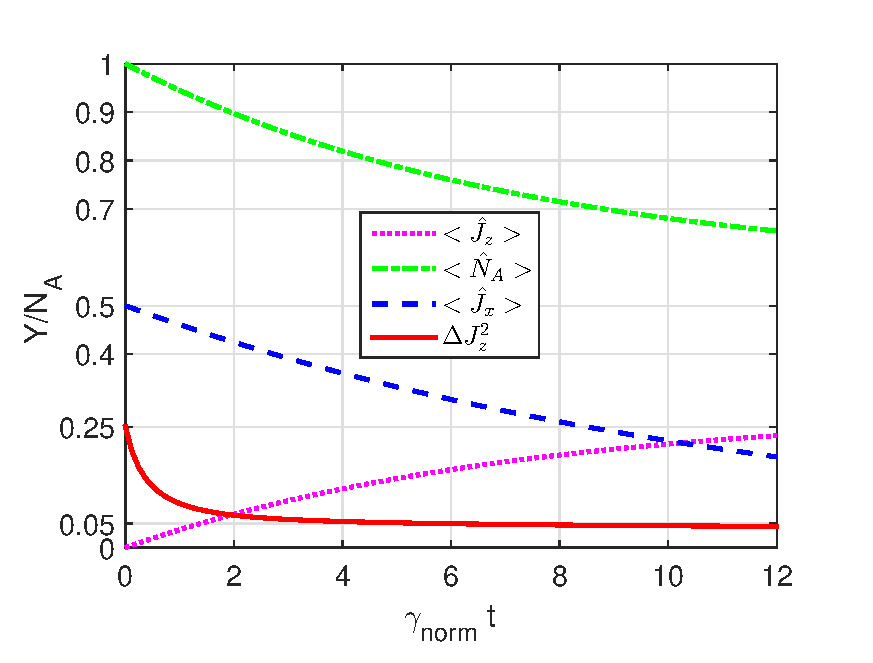
\includegraphics[scale=0.45]{../media/Figs/clockdynamics_m33_yq_rp1d5_exact}}
%\end{minipage}
%\begin{minipage}{.5\linewidth}
%\centering
%\subfloat[]{\label{fig:clockdynamics_m33_yq_rp1d5_approx}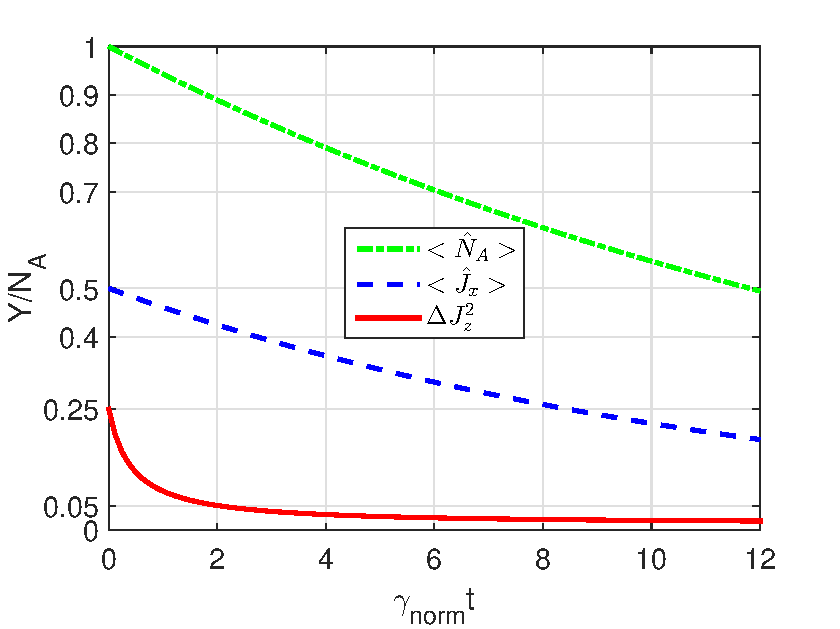
\includegraphics[scale=0.45]{../media/Figs/clockdynamics_m33_yq_rp1d5_approx}}
%\end{minipage}
%\par\medskip
%\begin{minipage}{.5\linewidth}
%\centering
%\subfloat[]{\label{fig:clockdynamics_m44_yq_rp1d5_exact}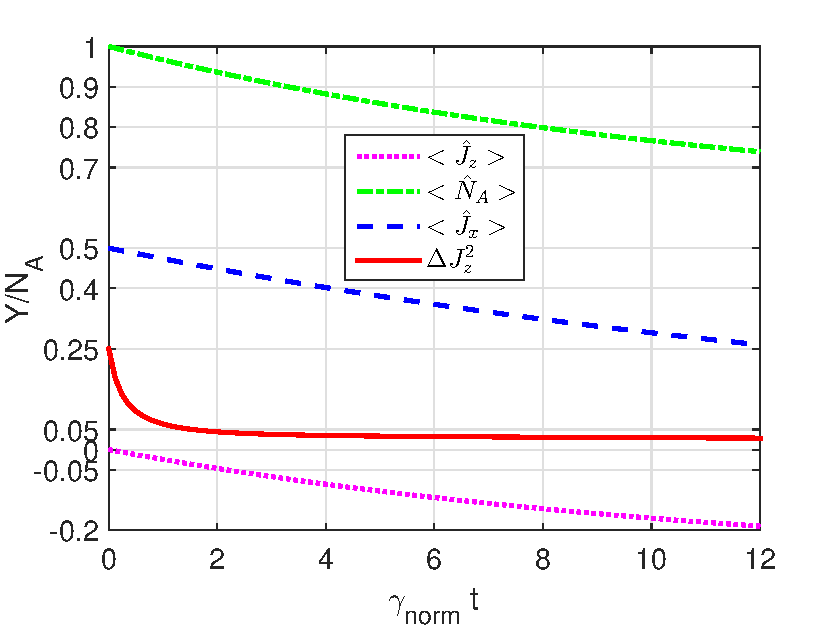
\includegraphics[scale=0.45]{../media/Figs/clockdynamics_m44_yq_rp1d5_exact}}
%\end{minipage}
%\begin{minipage}{.5\linewidth}
%\centering
%\subfloat[]{\label{fig:clockdynamics_m44_yq_rp1d5_approx}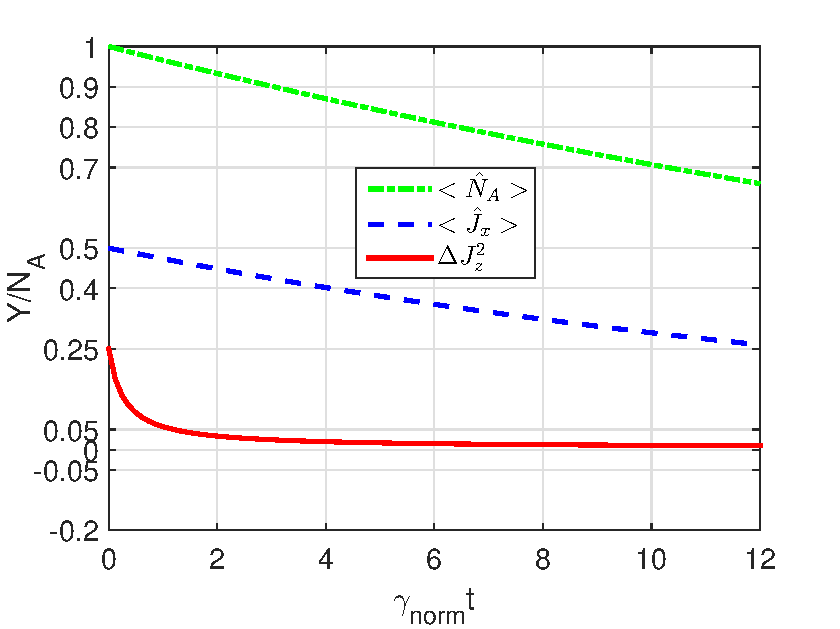
\includegraphics[scale=0.45]{../media/Figs/clockdynamics_m44_yq_rp1d5_approx}}
%\end{minipage}
%\caption{Evolution of expectation values of collective spin operators as a function of time with $ N_A=1000 $ atoms trapped at $ r'\!_\perp =1.5a $ along the $ H/x $ axis of the nanofiber. Subfigs.~\protect\subref{fig:clockdynamics_m33_yq_rp1d5_exact} and~\protect\subref{fig:clockdynamics_m33_yq_rp1d5_approx} use the magic frequencies close to the $ F=3\leftrightarrow F'=3 $ transition frequency $ \omega_{33'} $. Subfigs.~\protect\subref{fig:clockdynamics_m44_yq_rp1d5_exact} and~\protect\subref{fig:clockdynamics_m44_yq_rp1d5_approx} used the magic frequencies close to $ \omega_{44'} $. The $ \phi $ axis was defined as the quantization axis for these plots. Subfigs.~\protect\subref{fig:clockdynamics_m33_yq_rp1d5_exact} and~\protect\subref{fig:clockdynamics_m44_yq_rp1d5_exact} were calculated using the exact solution of the coupled differential equations of the expectation values of spin operators. In contrast, Subfigs.~\protect\subref{fig:clockdynamics_m33_yq_rp1d5_approx} and~\protect\subref{fig:clockdynamics_m44_yq_rp1d5_approx} use approximations by ignoring the dynamics of $ \expect{\hat{J}_z} $ for all calculations, and treat $ \expect{\hat{N}_C} $ as a constant in solving the differential equation for $ \Delta J_z^2 $. Other parameters used: $ \Omega/2\pi=52 $ MHz (does not matter). }\label{fig:clockdynamics_m_yq_rp1d5}
%\end{figure}

%\begin{figure}
%\begin{minipage}{.5\linewidth}
%\centering
%\subfloat[]{\label{fig:xi_magic33_yq}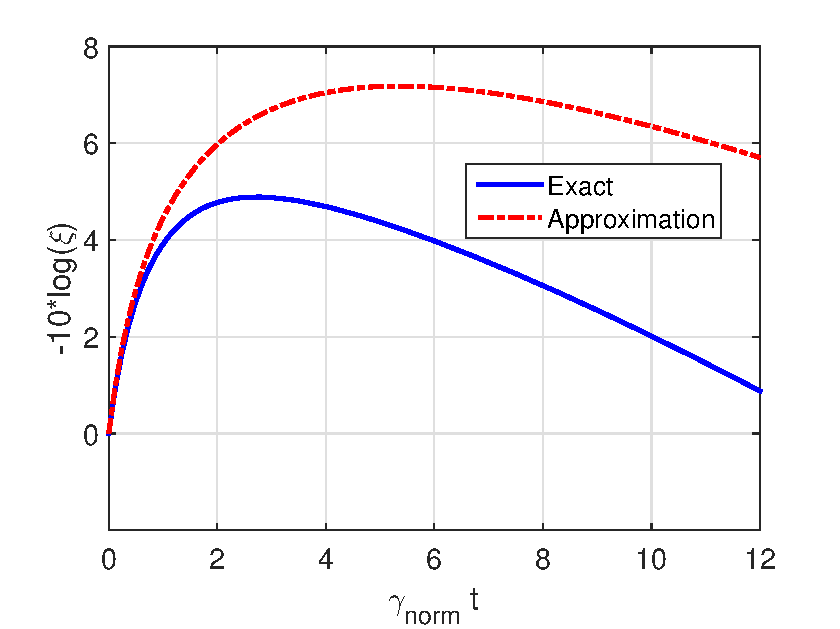
\includegraphics[scale=0.45]{../media/Figs/xi_magic33_yq}}
%\end{minipage}
%\begin{minipage}{.5\linewidth}
%\centering
%\subfloat[]{\label{fig:xi_magic44_yq}\includegraphics[scale=0.45]{../media/Figs/xi_magic44_yq}}
%\end{minipage}
%\par\medskip
%\begin{minipage}{.5\linewidth}
%\centering
%\subfloat[]{\label{fig:xi_magic33_xq}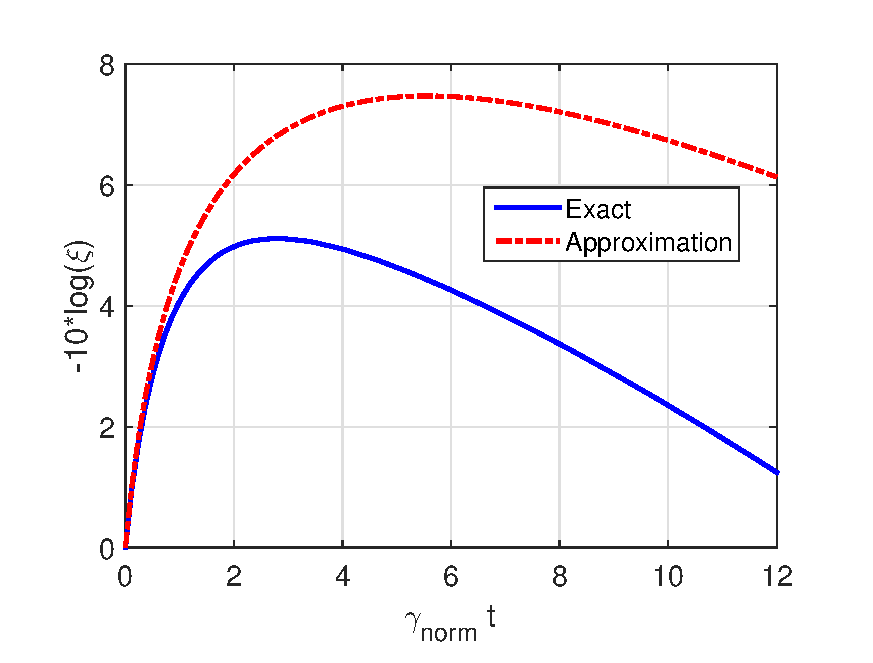
\includegraphics[scale=0.45]{../media/Figs/xi_magic33_xq}}
%\end{minipage}
%\begin{minipage}{.5\linewidth}
%\centering
%\subfloat[]{\label{fig:xi_magic44_xq}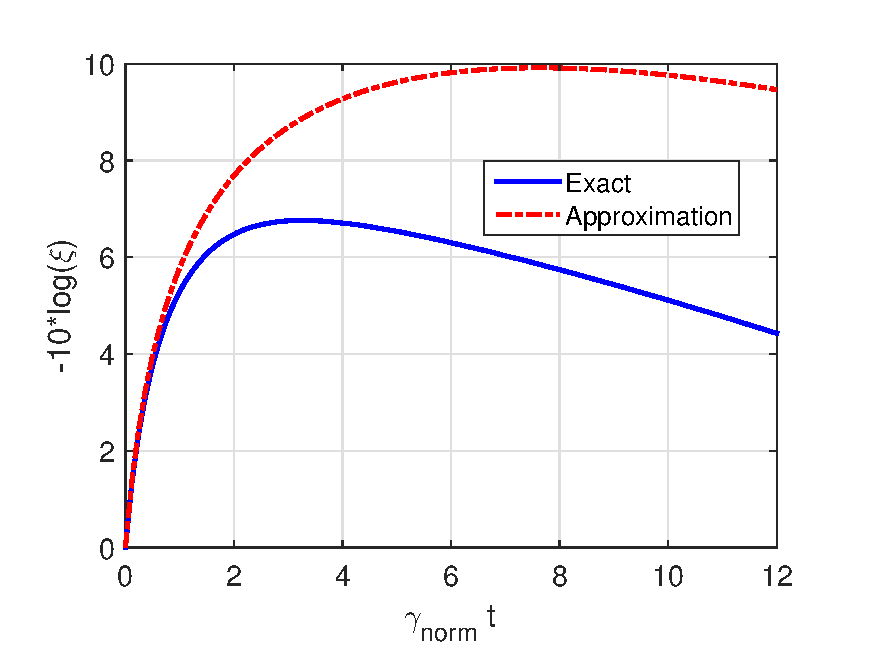
\includegraphics[scale=0.45]{../media/Figs/xi_magic44_xq}}
%\end{minipage}
%%\centering\makebox[\textwidth]{
%%\includegraphics[width=0.65\textwidth]{./Figs/xi_magic44_yq}}
%\caption{Spin squeezing evolution as a function of time with $ N_A=1000 $ atoms trapped at $ r'\!_\perp =1.5a $ along the $ H/x $ axis of the nanofiber. Subfigs.~\protect\subref{fig:xi_magic33_yq} and~\protect\subref{fig:xi_magic33_xq} use the magic frequencies close to the $ F=3\leftrightarrow F'=3 $ transition frequency $ \omega_{33'} $. Subfigs.~\protect\subref{fig:xi_magic44_yq} and~\protect\subref{fig:xi_magic44_xq} used the magic frequencies close to $ \omega_{44'} $. The magic frequencies and spin squeezing parameters are different for different choices of quantization axis. Subfigs.~\protect\subref{fig:xi_magic33_yq} and~\protect\subref{fig:xi_magic44_yq} define $ \phi $ axis as the quantization axis. In contrast, subfigs.~\protect\subref{fig:xi_magic33_xq} and~\protect\subref{fig:xi_magic44_xq} use $ r\!_\perp $ axis as the quantization axis. When $ z $ axis is chosen to be the quantization axis, almost no squeezing effect can be observed at the magic frequencies. As can be seen, when the quantization axis close to the local field direction, the spin squeezing parameter can reach to a higher value. Other parameters used: $ \Omega/2\pi=52 $ MHz (does not matter). }\label{fig:xi_magic}
%\end{figure}

%</birefringencemotioneq>

%\bibliography{Nanofiber}
%\bibliographystyle{amsplain}
\bibliographystyle{../styles/abbrv-alpha-letters-links}
%\bibliographystyle{unsrt}
% \nocite{*}
\bibliography{../refs/Archive,../chap4/Nanofiber}

\printindex

\end{document}          


